\chapter{機械学習を用いたCoincidence Windowの作成手法}\label{chapter4}
第\ref{chapter3}ではATLAS実験で実装されているトリガーシステムの概要について説明し、初段ミューオントリガーで使用されているCWの作成及びRun-2における最適化手法について述べ、効率的な最適化手法の開発が必要であることを示した。
本章では近年発展が著しい機械学習についての概説を述べ、本研究の主題である機械学習を用いた効率の良いCWの作成及び最適化手法について述べる。

\section{機械学習}\label{回帰分析}
コンピュータ自身がデータから「ルールや知識を獲得」(学習)するアプローチを機械学習と呼ぶ。そして、学習した結果を用いて予測や認識、作成など様々なタスクを行うことができる。「複数人の専門家が数年かかって作っていく」ようなルールや知識などは、作成自体にも、作成後の調整や変更にも膨大な時間とコストがかかるが、機械学習を用いることで学習用のデータを機械にかけて数日待てば自動的に作成することができるのである。
機械学習が行う代表的なタスクとして「クラス分類」と「回帰分析」がよく知られている。
クラス分類とは、分析したいデータが属するカテゴリーやクラス、種類が何なのかを予測する手法である。特に、予測するクラス数が 2 クラスの場合には 2 値分類と、2クラスより多い分類予測については多クラス分類と呼ばれる。図~\ref{fig:class}にクラス分類の概要図を示す。高エネルギー物理学実験では、粒子の同定や探索の対象としている信号事象 (シグナル) とその背景事象 (バックグラウンド) の分離などに応用されている。
回帰の主な目的は、連続値などの値を学習データの傾向をもとに予測することである。過去の気温から明日の気温を予測することや企業における売り上げの予測などが回帰に当てはまる。
回帰分析には、線形回帰、多項式回帰などが存在し、図~\ref{fig:regre}に線形回帰の概要図を示す。回帰問題では、入力データを線形関数もしくは多項式関数を用いて近似することで、データの傾向を表す関数を作成する。高エネルギー物理学実験では、粒子の衝突で得られたデータを入力変数とし、粒子のエネルギー測定の補正を行う解析などに応用されている。

\begin{figure}[tb]
  \centering
    \begin{minipage}[b]{0.4\linewidth}
        \centering
        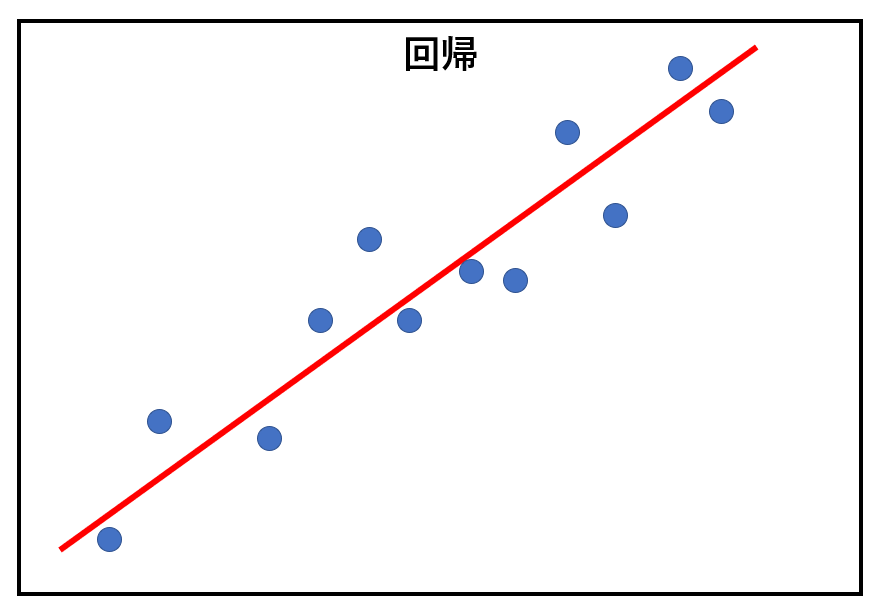
\includegraphics[clip, width=7cm]{fig/4/regression.png}
        \vspace{10pt}
        \subcaption{}
        \label{fig:regre}
    \end{minipage}
    \hfill
    \begin{minipage}[b]{0.4\linewidth}
        \centering
        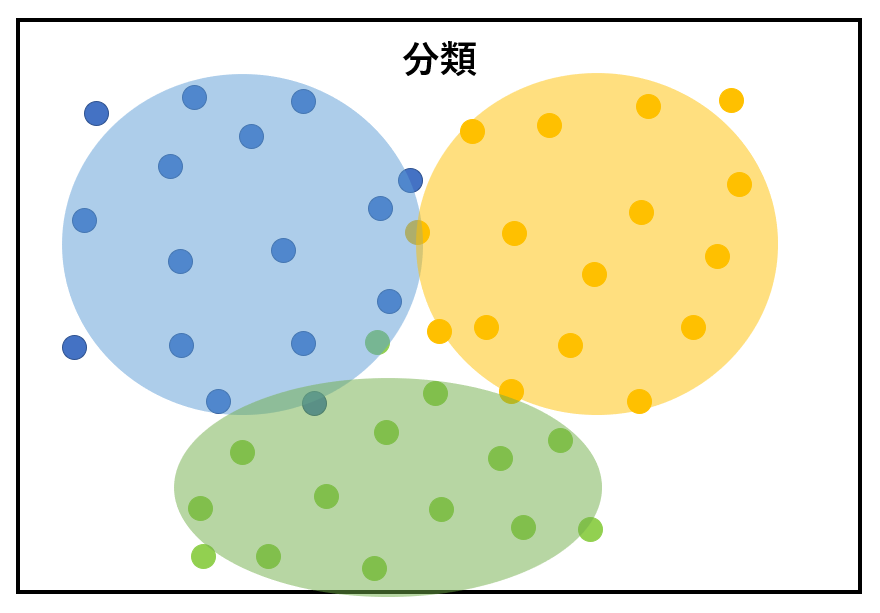
\includegraphics[clip, width=7cm]{fig/4/classification.png}
        \vspace{10pt}
        \subcaption{}
        \label{fig:class}
    \end{minipage}
  \caption{機械学習の代表的な分析手法。(a):回帰分析、(b):クラス分類の概要図}
  \label{fig:fit_def}
\end{figure}

機械学習の学習手法は、正解の値(教師データ)を与えた状態で傾向を学習させる「教師あり学習」と教師データを用いずに学習を行う「教師なし学習」の2つに大きく分けられる。
最も広く使われている学習手法である教師あり学習は、正解のデータが用意されており、正しい出力ができるように入力データの特徴やルールを学習していく手法である。教師あり学習は、既存のデータをもとに、タスクごとに設定されたいくつかのクラスに識別する「クラス分類」と、連続する値を予測する「回帰分析」を行うことができる。本研究では「教師あり学習」によるトレーニングを行い「回帰分析」による連続値の予測に着目する。
%教師あり学習は正解の値を与えた状態で傾向を学習させる方法である。
%教師あり学習は、「学習」と「予測」といった 2 つのプロセスによって成り立っており、、正解のデータを用いてルールやパターンの学習を行った後、新しいデータに対して、これまでに学習したデータを用いて予測を行う。
%一方で教師なし学習は、正解の値を教えずに学習させる方法である。大量のデータを学習させることでデータの特徴やパターンなどを覚えるが、それが正解か否かを判断することを学ぶのが教師なし学習の特徴である。
%また強化学習では、出力される結果に点数をつけて、最も多くの点数を得るための行動を学習させる。教師なし学習と同じように正解の値を学習させないが、教師なし学習との違いは、機械が報酬を得るために最適な行動を自ら考え実行する点である。

\subsection{ニューラルネットワーク}
機械学習には多くの種類があるが、その内の一つがニューラルネットワークを使った手法である。ニューラルネットワークとは、人間の脳内にある神経細胞(ニューロン)とそのつながり、つまり神経回路網を人工ニューロン(パーセプトロン)という数式的なモデルで表現したものである。個々のパーセプトロンは単純な仕組みであるが、多数組み合わせる事で複雑な関数近似を行う事ができるのが、ニューラルネットワークの大きな特徴である。
パーセプトロンを複数組み合わせ多層化し、複雑な表現を可能としたものを多層パーセプトロン~(MLP : Multilayer perceptron)と呼ぶ。

図~\ref{fig:perce}に示すように、一つ一つのパーセプトロンは入力と出力で構成される。パーセプトロンでは、式~\eqref{equ:input}で表すように、n個の入力変数$x_i$に対し重み$w_i$を作用させバイアスbを足し合わせた入力値aが、関数$f(a)$によって変換され出力値yとして出力される。このバイアスbと重み$w_i$のパラメータを調節することで、様々な出力が可能となる。
\begin{figure}[tb]
  \centering
  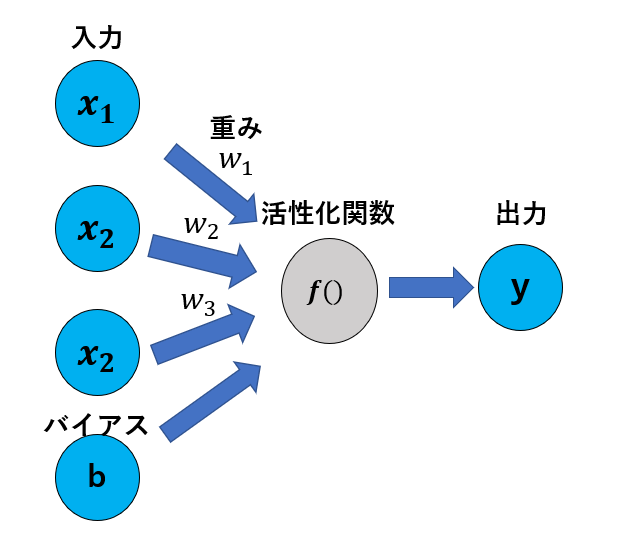
\includegraphics[clip, width=13cm]{fig/4/parceptron.png}
  \caption{単一パーセプトロンの概念図。}
  \label{fig:perce}
\end{figure}
このとき、式~\eqref{equ:activation}で表す$f(a)$の事を「活性化関数」と呼び、活性化関数には、sigmoid関数、tanh関数、ReLU関数~(Rectified Linear Unit)」、softmax関数などが良く使われている。
sigmoid関数及びReLU関数の概形を図~\ref{fig:sigmoid}、図~\ref{fig:ReLU}に示す。sigmoid関数はニューラルネットワークでよく用いられてきた関数であり、式~\eqref{equ:sigmoid}のような関数で表される。ReLU関数は式~\eqref{equ:ReLU}のような関数で示される。
\begin{equation}
    y = \frac{1}{1+exp(-x)}
    %f \begin{pmatrix}  \\ 2 & 3 \end{pmatrix}
    \label{equ:sigmoid}
\end{equation}

\begin{equation}
    y = max(0,x)
    %f \begin{pmatrix}  \\ 2 & 3 \end{pmatrix}
    \label{equ:ReLU}
\end{equation}

\begin{figure}
    %\centering
    \begin{tabular}{cc}
    \begin{minipage}[b]{0.45\hsize}
        %\centering
        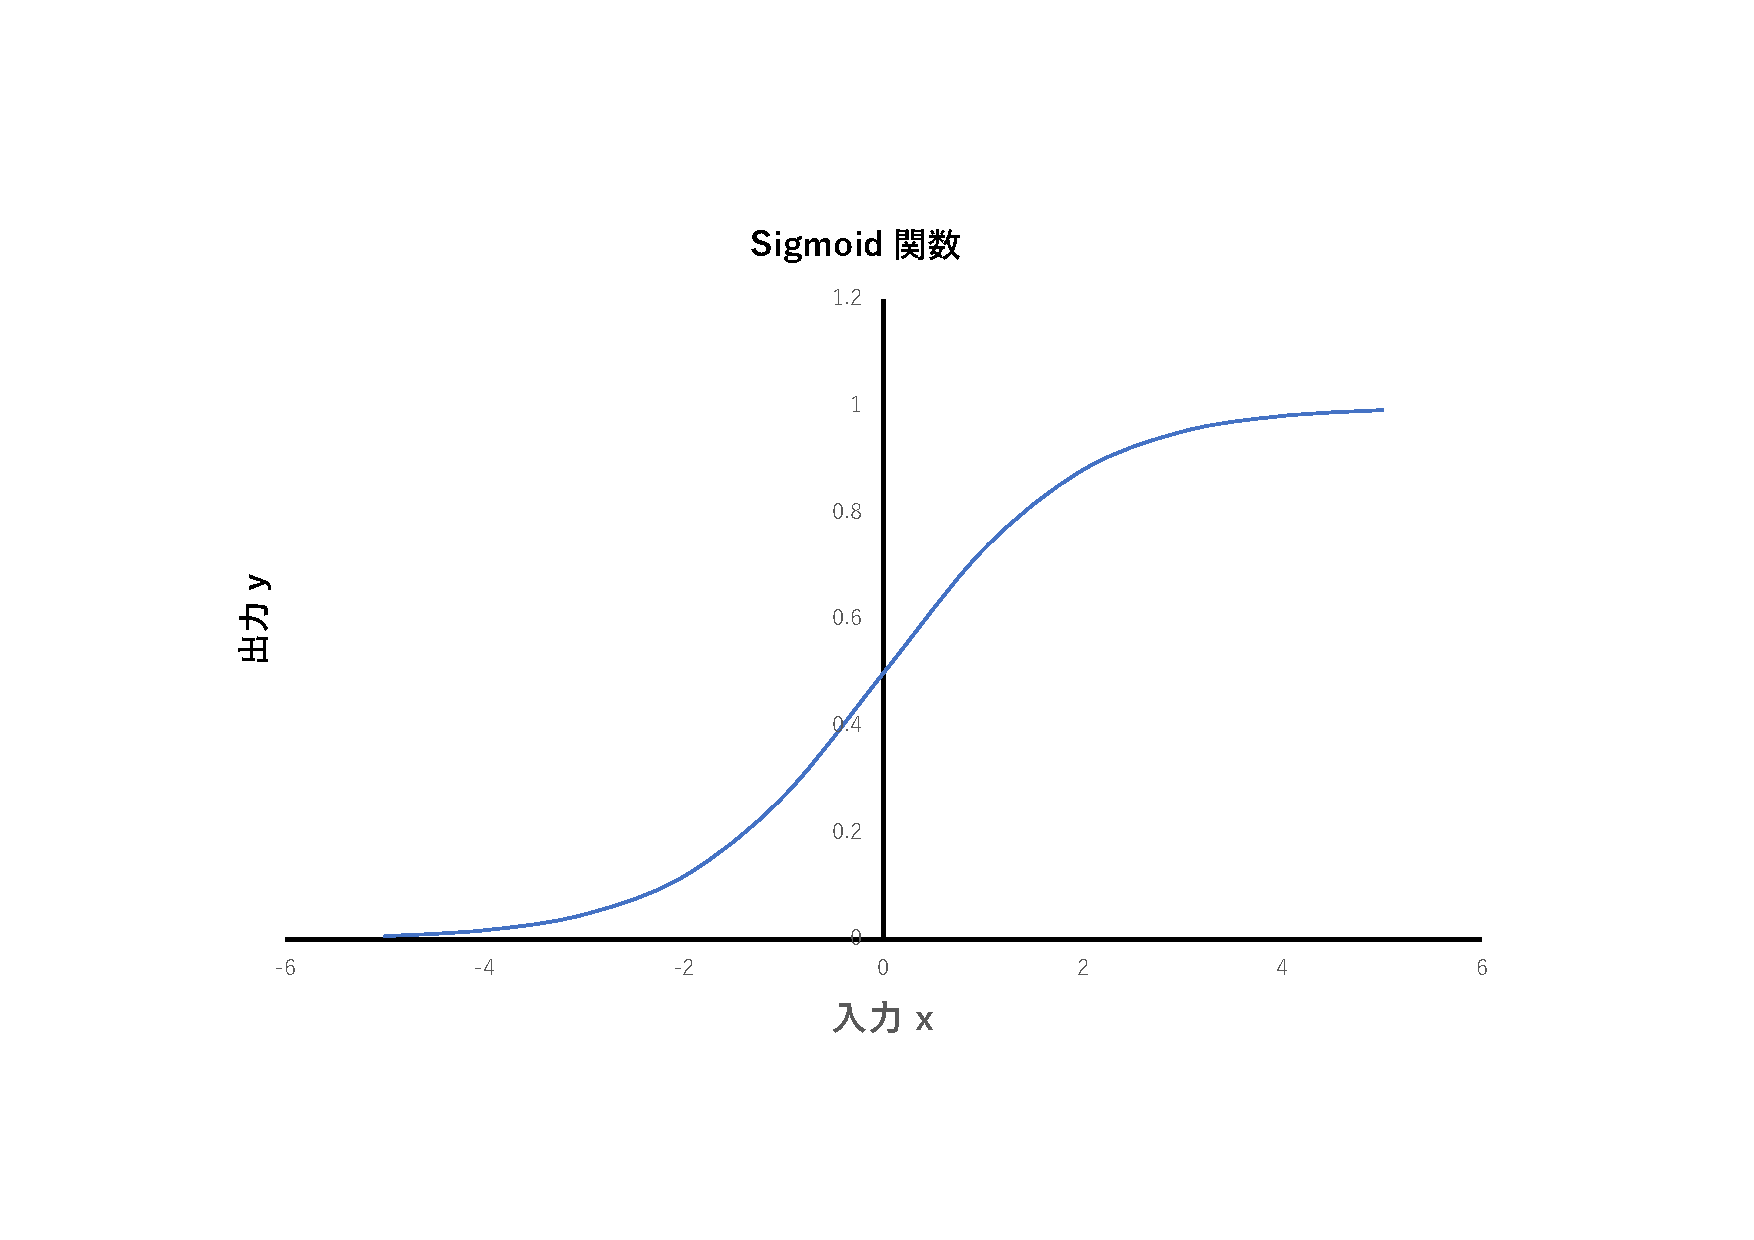
\includegraphics[clip, width=7cm]{fig/4/sigmoid_2.pdf}
        %\vspace{5pt}
        \subcaption{}
        \label{fig:sigmoid}
    \end{minipage}&
    %\hfill
    \begin{minipage}[b]{0.45\hsize}
        %\centering
        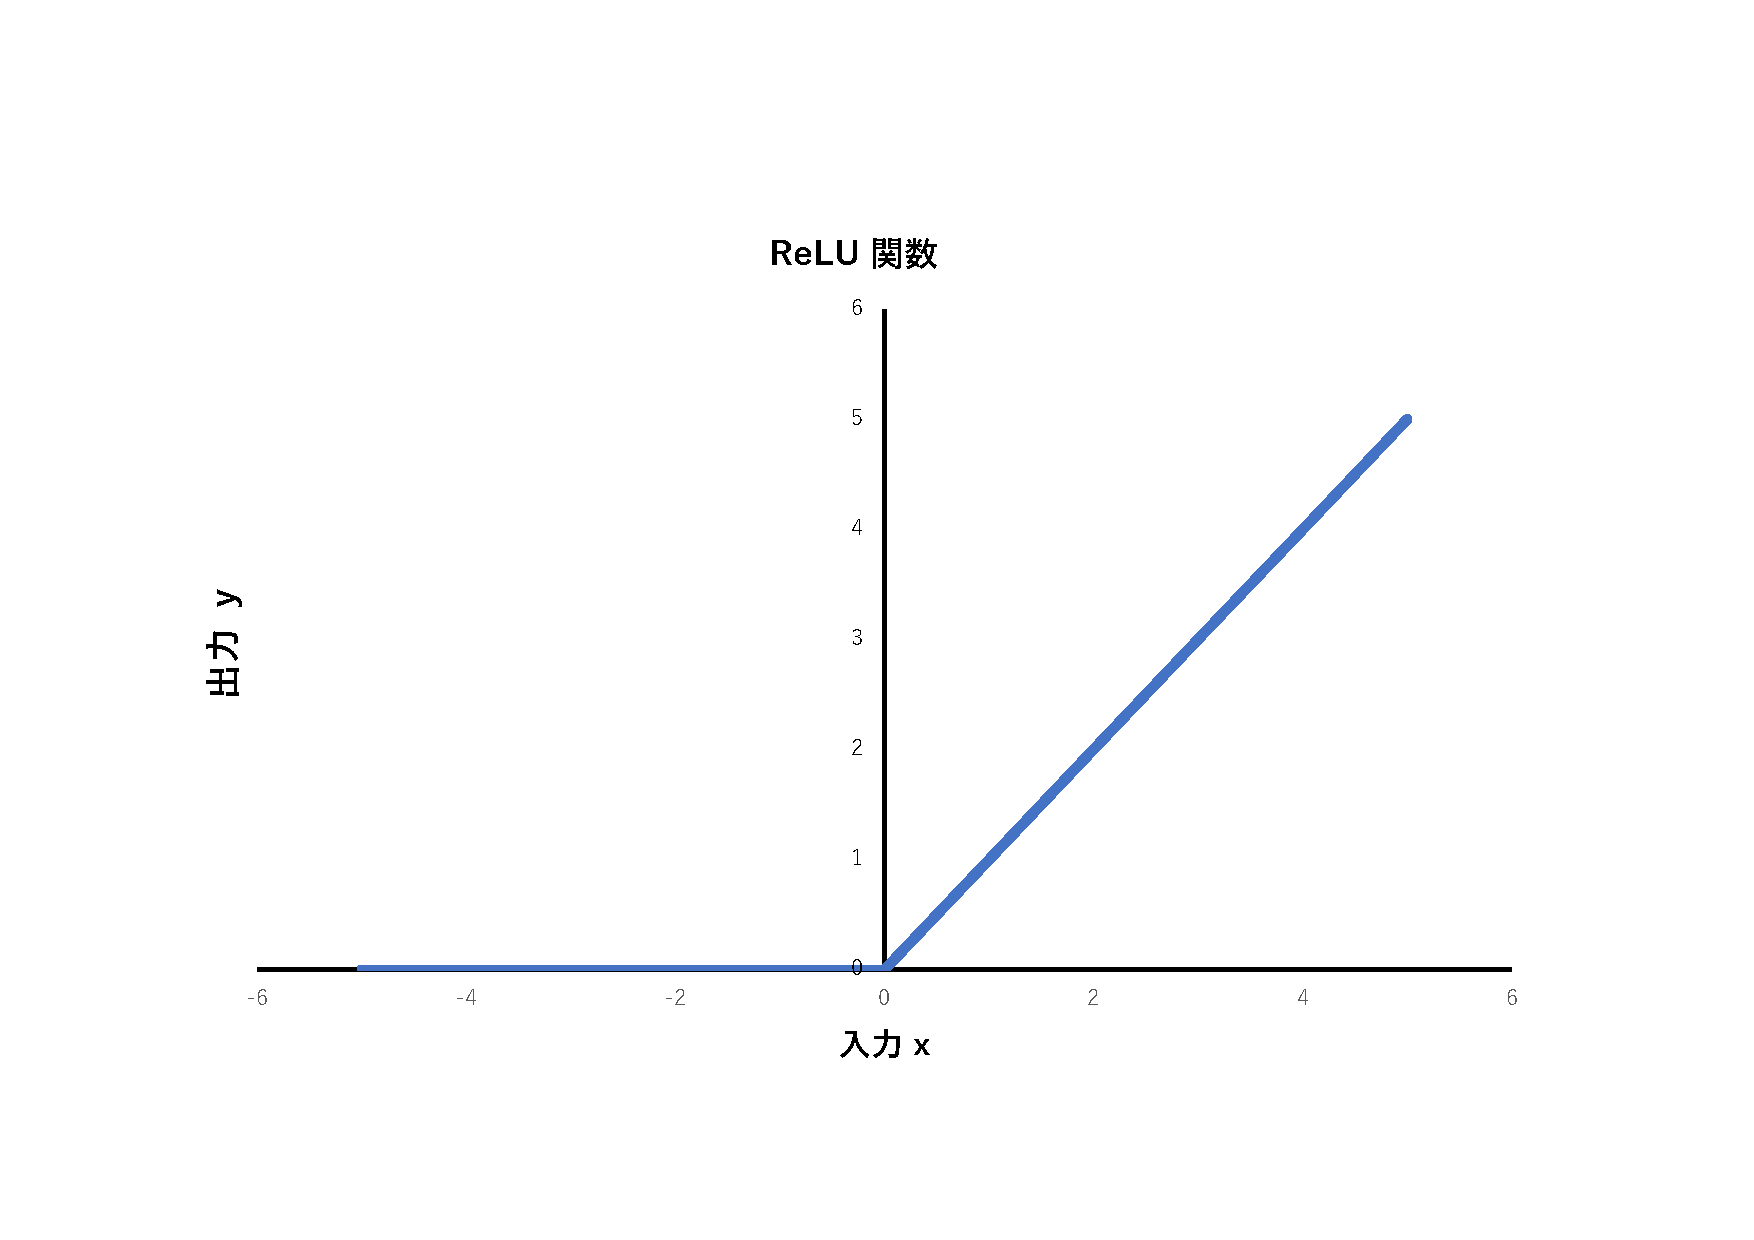
\includegraphics[clip, width=7cm]{fig/4/ReLU_2.pdf}
        %\vspace{5pt}
        \subcaption{}
        \label{fig:ReLU}
    \end{minipage}
    \end{tabular}
    \caption{機械学習で用いられる活性化関数の例。(a): sigmoid 関数、(b): ReLU 関数。}
    \label{fig:acctivation}
\end{figure}
\begin{eqnarray}
    a &=& \sum^{n-1}_{i=1}(x_i・w_i) + b \label{equ:input}\\
    y &=& f(a)\label{equ:activation}
\end{eqnarray}

このような、パーセプトロンを図~\ref{fig:MLP}に示すように複数組み合わせたものがMLPである。
\begin{figure}[tb]
  \centering
  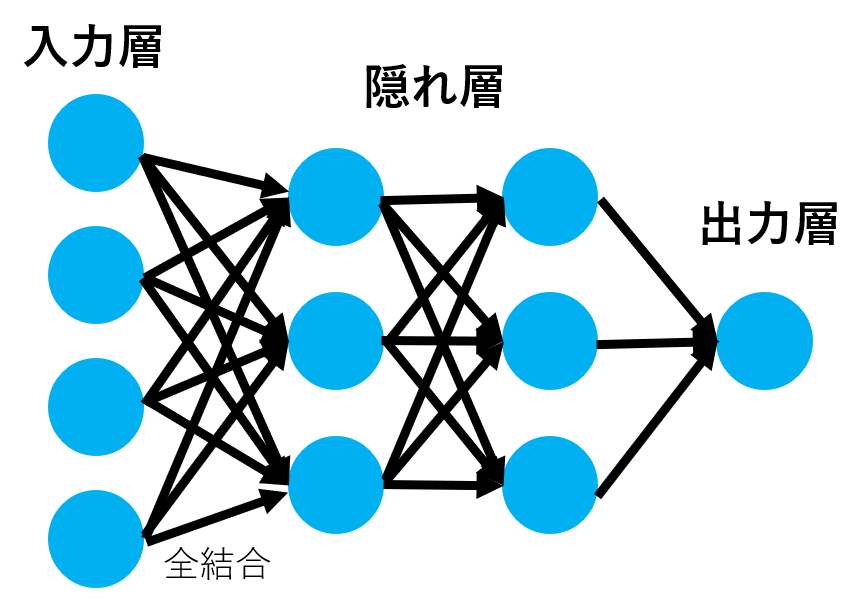
\includegraphics[clip, width=10cm]{fig/4/MLP_re.png}
  \caption{MLP の概形。パーセプトロンを複数組み合われており、ある層のパーセプトロンからの出力は全結合されて次の層の各パーセプトロンに入力される。}
  \label{fig:MLP}
\end{figure}

\subsubsection{多層パーセプトロン}
MLPは隠れ層と呼ばれる層が複数追加されたネットワーク構造を持ち、各層の間は全結合しているような構造になっている。この様な構造を持つニューラルネットワークの事を「全結合型ニューラルネットワーク」と呼ぶ。
このように、MLPはパーセプトロンを複数接続したことにより、調整可能なパラメータが増加し、MLP全体として複雑な出力が可能となった。
そこで教師あり学習では、入力変数に対する出力ができる限り教師データと一致するようなパラメータ($w_i$,b)を求めることで学習を行う。
このようなパラメータは、「最適化問題を解く」ことで求めることができる。最適化問題とは変数a、bとある関数$L(a,b)$が与えられたとき、関数の値が最小となるような変数の組(a,b)を探す問題である。
この$L(a,b)$は「損失関数」と呼ばれ、学習データで与えられる正解値に対し、予測がどれだけ間違っているのかを評価する関数である。具体的には、学習データからの入力$x_n$に対して設定したパラメータ($w$,b)の時の予測値$y$を、損失関数を用いて正解値$t$と比較することで予測精度を表現することができる。
損失関数は主に、予測が正しいほど小さい値を返すような関数が用いられ、特に式~\eqref{equ:MSE}に示すような関数で表される平均二乗誤差~(MSE : Mean Squared Error)が多く用いられる。他には、平均絶対誤差~(MAE : Mean Absolute Error)や平均二乗誤差の平方根~(RMSE : Root Mean Squared Error)などが用いられる。
\begin{equation}
    L = \frac{1}{n}\sum^{n}_{i=1}(y_i-t_i)^2
    %f \begin{pmatrix}  \\ 2 & 3 \end{pmatrix}
    \label{equ:MSE}
\end{equation}
機械学習のトレーニングでは、この損失関数の値が最小になるようにパラメータの値を増減させて調整を行う。そして、機械学習による予測と損失関数による評価を繰り返すことによって予測の精度を向上させていく。このパラメータを更新していく方法を勾配降下法と呼ぶ。図\ref{fig:lossfunction}に勾配降下法によるパラメータの更新の流れを示す。

勾配降下法は現在のパラメータ$w_i$における勾配$\frac{\partial L}{\partial w_i}$を求め、パラメータを
\begin{equation}
    w_{i+1} = w_i - \eta\frac{\partial L}{\partial w_i}
    \label{equ:勾配}
\end{equation}
と更新する。ここで、$\eta$は学習率~(Learning rate)と呼ばれ、一度のパラメータの更新で変更する値の大きさを表す。そして、新しく設定したパラメータでの勾配を求め、さらに更新していくことで、損失関数が小さくなる方向にパラメータを調節することができる。この更新を行う回数をepochと呼び、学習率などと合わせて人間が設定する値をハイパーパラメータと呼ぶ。


\begin{figure}[tb]
  \centering
  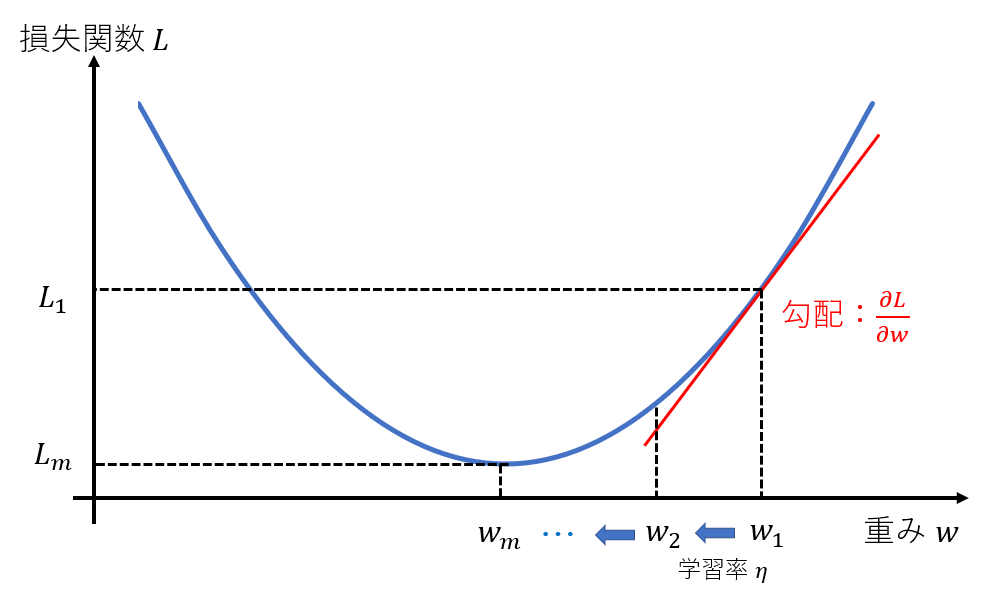
\includegraphics[clip, width=10cm]{fig/4/lossfunc_laerning.png}
  \caption{損失関数$L$の最小化の流れ。ある重み$w_i$の時の勾配$\frac{\partial L}{\partial w}$を計算し、この勾配が小さくなるように重みを更新することを繰り返す。この際、更新量を調整するために学習率$\eta$を設定する。バイアス$b$に対しても同様に最小化を行う。}
  \label{fig:lossfunction}
\end{figure}



\section{機械学習を用いたCW作成手法}
本節では機械学習の学習方法及びCWを作成する手法について述べる。
従来の作成手法では、シミュレーションデータを用いて$p_{\rm{T}}$閾値を決定しCWを作成する。その後、実際のデータを使用して磁場の影響や検出器のズレに最適化させるといった方法を行っていた。一方、本研究で開発する作成手法では実際のデータを学習に利用した機械学習を用いてミューオンの$p_{\rm{T}}$の予測を行い、予測した$p_{\rm{T}}$を使用してCWを作成する。また、本研究で作成するCWは実際の測定で用いるトリガー用のCWの他にシミュレーションで用いるトリガー用のCWもシミュレーションデータを用いて同様の手法で作成する。

初めに、トレーニングに使用するシミュレーションデータおよび実際のデータを学習に適した形式に変更する。次に図~\ref{fig:MLP_over}に示すように、TGCにおけるミューオンのヒット位置の情報と、ミューオンの飛跡の曲がり具合の4変数から$p_{\rm{T}}$の値を出力するMLPをトレーニングする。この時、機械学習の分析手法として回帰分析を行うため、出力される値は連続値となる。出力された$p_{\rm{T}}$の値を15段階の閾値に変換するために、任意の値で$p_{\rm{T}}$を区切り、トリガー効率を求めTurn-on curveにフィッティングを行うことで15段階の$p_{\rm{T}}$閾値に対応したCWを作成する。

\begin{figure}[tb]
  \centering
  \hspace*{-1cm}
  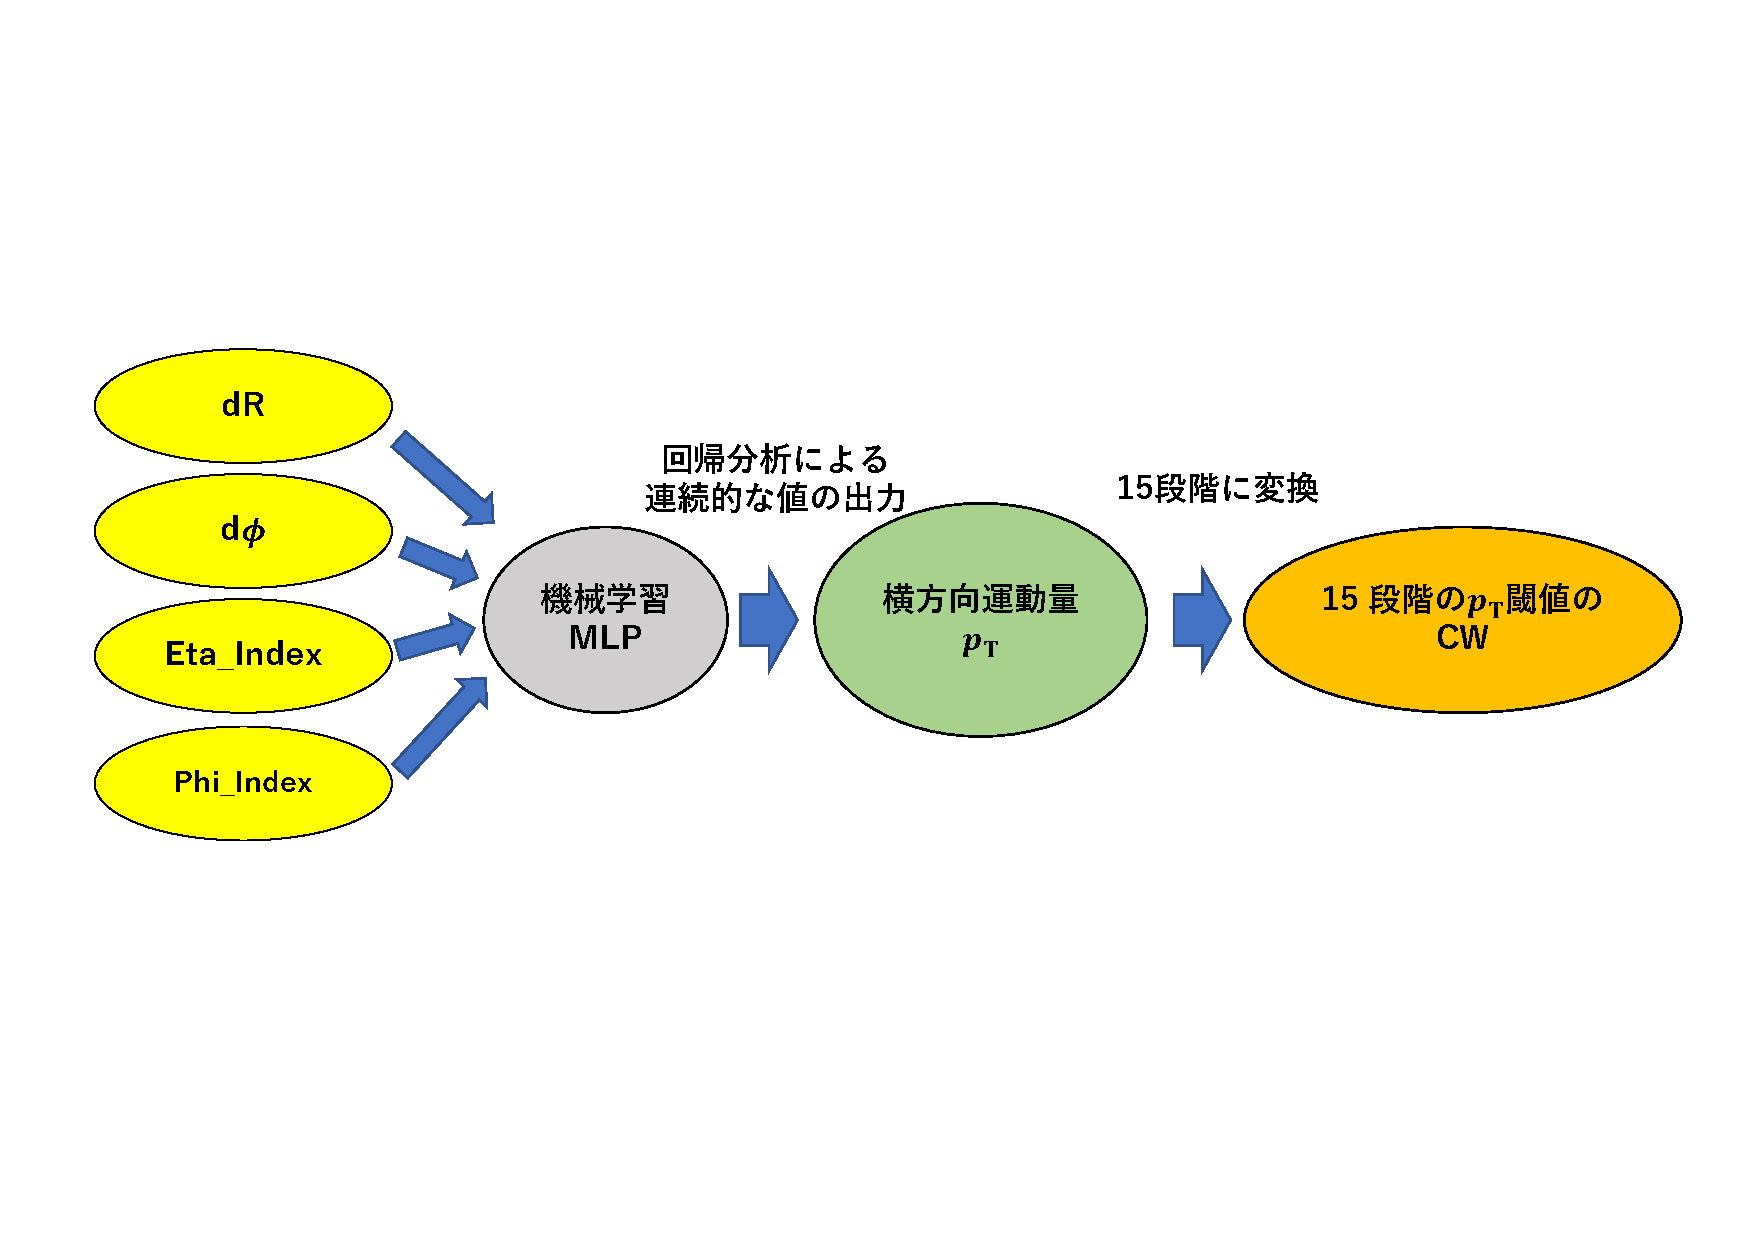
\includegraphics[clip, width=15cm]{fig/4/MLPoverview2.pdf}
  \caption{機械学習を用いたCW作成の流れ。dR、d$\phi$、Eta$\_$Index、Phi$\_$Indexの4変数を入力値、横方向運動量$p_{\rm{T}}$を出力値とした機械学習を用いる。出力された$p_{\rm{T}}$は連続値であり、これを15段階の$p_{\rm{T}}$閾値に変換することで CW を作成する。}
  \label{fig:MLP_over}
\end{figure}

\subsection{入力データに対する事前処理}\label{事前処理}
本節では学習に用いるシミュレーションデータおよび実際のデータに対して処理を行い、本研究の機械学習に適した形式に変換する方法について述べる。

本研究ではトレーニングのために、シミュレーションデータ及び実際の測定データを使用する。
シミュレーション用のCWを作成するための機械学習のトレーニングには、1回のイベントに対してミューオンが1個存在するシングルミューオンのシミュレーションサンプルを使用する。オフライン再構成されたミューオンに対して、TGCのM3におけるヒット情報が存在することを要求する。そして、TGC M3におけるヒット情報からヒット位置の情報(トリガーセクターの番号、RoIの番号)と飛跡の情報(dR、d$\phi$)を取得する。
また、実際の測定に使用するCWを作成するための機械学習のトレーニングには、2018年Run-2で収集されたデータを用いる。使用するイベントにはHLTのシングルミューオントリガーである「HLT$\_$mu26$\_$ivarmeduium」を要求する。シミュレーションデータと同様に、イベントの中でもTGC M3おけるヒット情報が存在するオフライン再構成されたミューオンをすべて使用し、TGC M3におけるヒット位置の情報(トリガーセクターの番号、RoIの番号)と飛跡の情報(dR、d$\phi$)を取得する。

%\begin{figure}[thb]
%  \centering
%  \rule{8cm}{6cm}
%  %\includegraphics[clip, width=14cm]{}
%  \caption{深層学習モデルのトレーニングに用いたシングルミューオンサンプルの $p_{\rm{T}}$分布。}
%  \label{fig:mu_pt_forMC}
%\end{figure}

%\begin{figure}[thb]
%  \centering
%  \rule{8cm}{6cm}
%  %\includegraphics[clip, width=14cm]{}
%  \caption{深層学習モデルのトレーニングに用いたミューオンの $p_{\rm{T}}$分布。}
%  \label{fig:mu_pt_forData}
%\end{figure}

\subsubsection{TGCの位置情報におけるナンバリングの変換}
学習には、TGCのヒット位置の情報としてトリガーセクターの番号とRoIの番号を使用する。
\ref{fig:TGCnumbering}に示すようにRoIはトリガーセクターごとに設定された番号が与えられており、あるトリガーセクターの一番端の列のRoIの番号は隣接するトリガーセクターのRoIの番号と関連性がない。
しかし、隣り合った場所に位置するRoIは似通った磁場構造を持っているため、トレーニングするにあたって、隣り合ったRoIの情報に関連性を持たせたい。

\begin{figure}[tb]
  \centering
  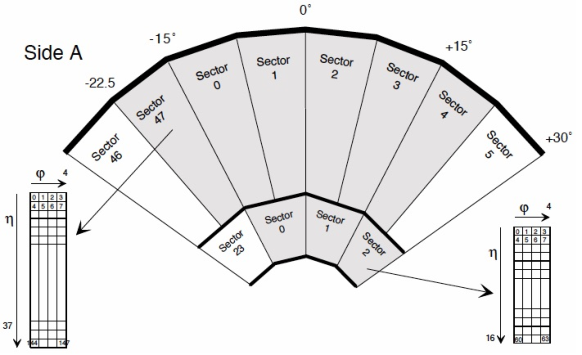
\includegraphics[clip, width=12cm]{fig/4/TGC_numbering.pdf}
  \caption{TGCにおけるトリガーセクターとRoIのナンバリングの概要。}
  \label{fig:TGCnumbering}
\end{figure}

本研究では、TGCにおけるヒット位置を表すトリガーセクターの番号とRoIの番号を、新たに隣り合ったRoIの番号が連続するようなナンバリングに変換する。
図~\ref{fig:newnumbering}に新たなナンバリングの概要を示す。Eta$\_$IndexはRoIを$\eta$方向に0から37の番号に、Phi$\_$IndexはRoIを$\phi$方向に0から191の番号に読み替えている。
\begin{figure}[tb]
  \centering
  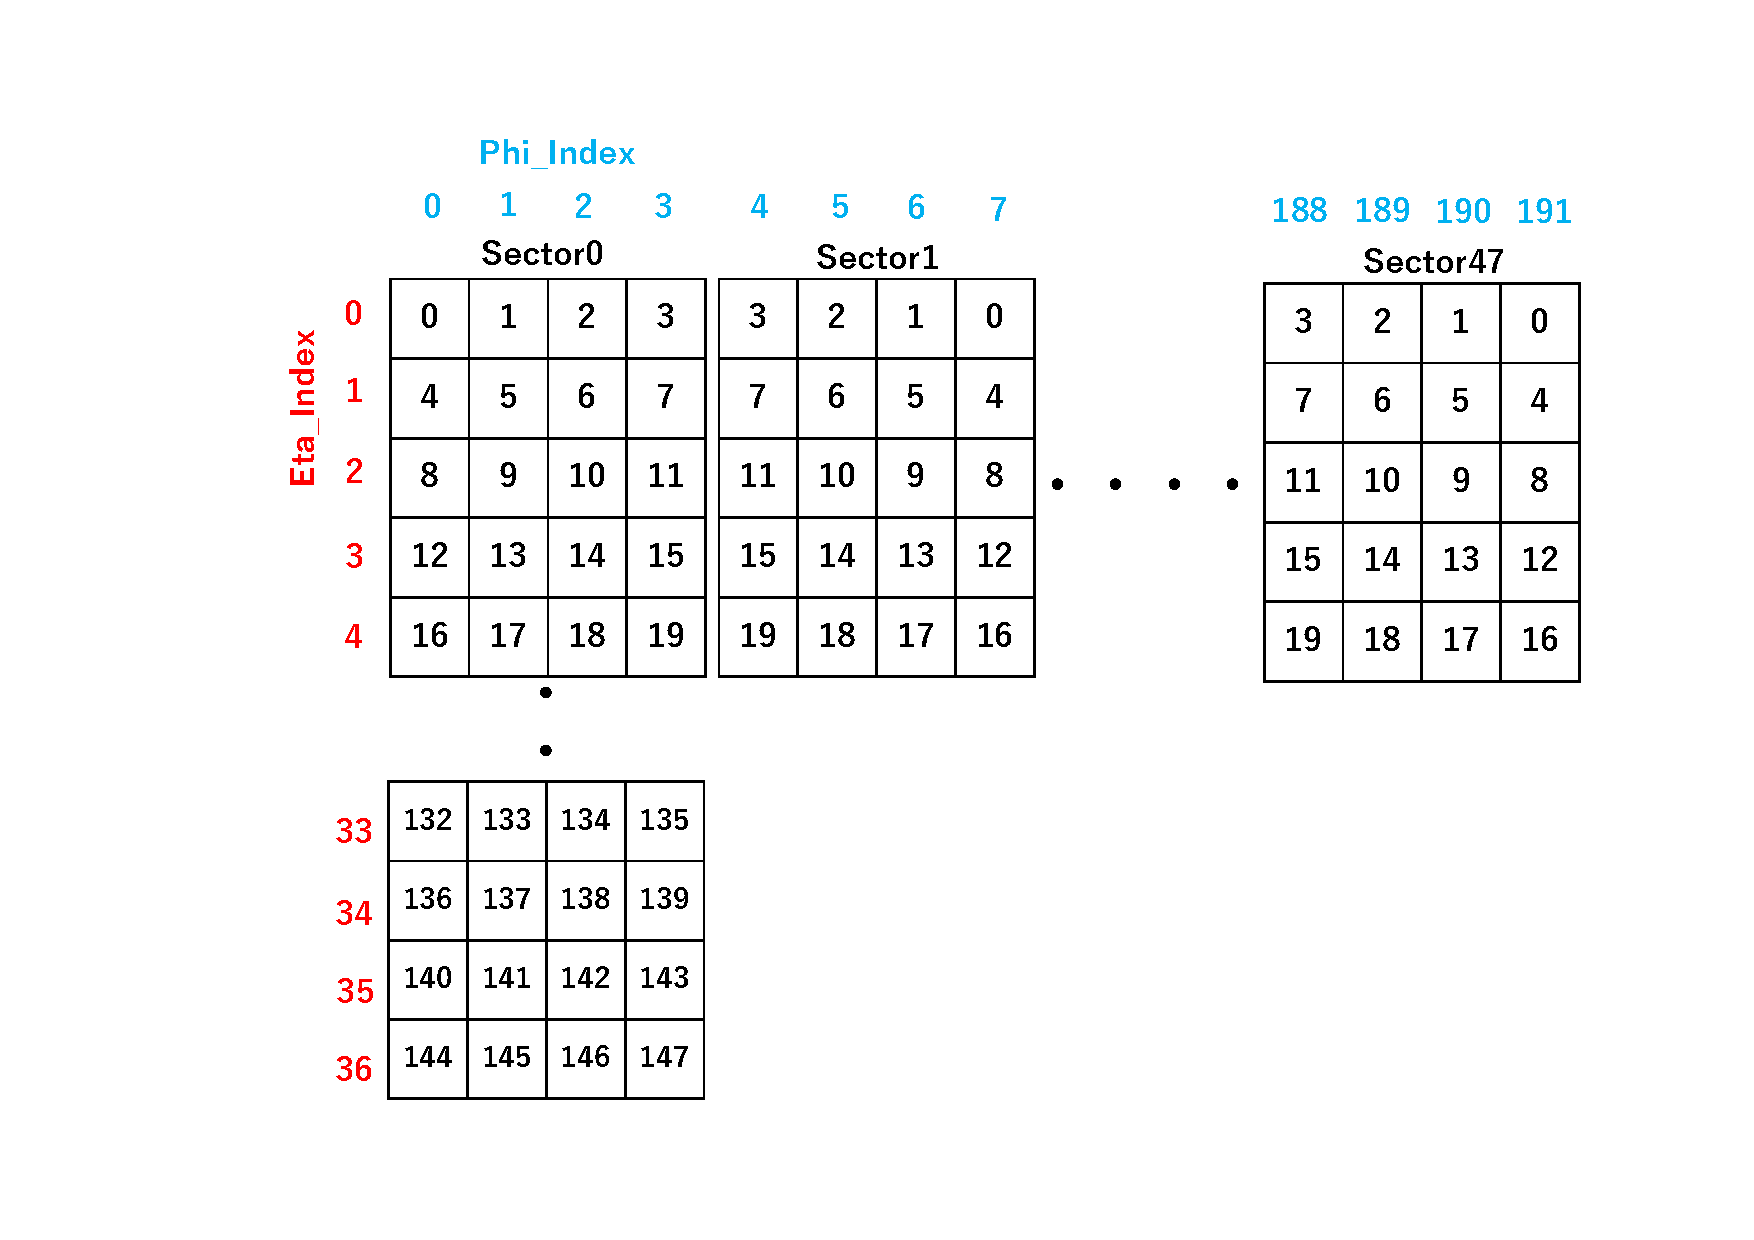
\includegraphics[clip, width=14cm]{fig/4/new_numbering.pdf}
  \caption{新たなナンバリングの概要。マスの中で数字はRoIの番号を表しており、奇数の番号のトリガーセクターでは読み出し回路の関係からRoIのナンバリング順が反転している。TGCにおけるヒット位置の情報(Sector番号、RoI番号)を新たに(Eta$\_$Index, Phi$\_$Index)で指定する。}
  \label{fig:newnumbering}
\end{figure}

\subsubsection{磁場構造を考慮した学習領域の分割}
\ref{magnetic_filed}節で述べたように、トロイド磁石が8回転対象に設置されていることにより TGC-BW における磁場構造は図\ref{fig:Mag}に示すように一様ではない。そのため、本研究ではTGC-BWの全領域を一つの機械学習でトレーニングさせるのではなく、図\ref{fig:Mag}で色付けされた領域が示すように、入力データとして使用する領域を分割して複数の機械学習をトレーニングする。
本研究では、磁場構造に考慮するためにTGC のエンドキャプ部を $\phi$方向に 48 分割、$\eta$方向に 9 分割、フォワード部を $\phi$方向に 24 分割、$\eta$方向に 4 分割にし、それぞれの領域に対して機械学習のトレーニングを行う。
\begin{figure}[tb]
  \centering
  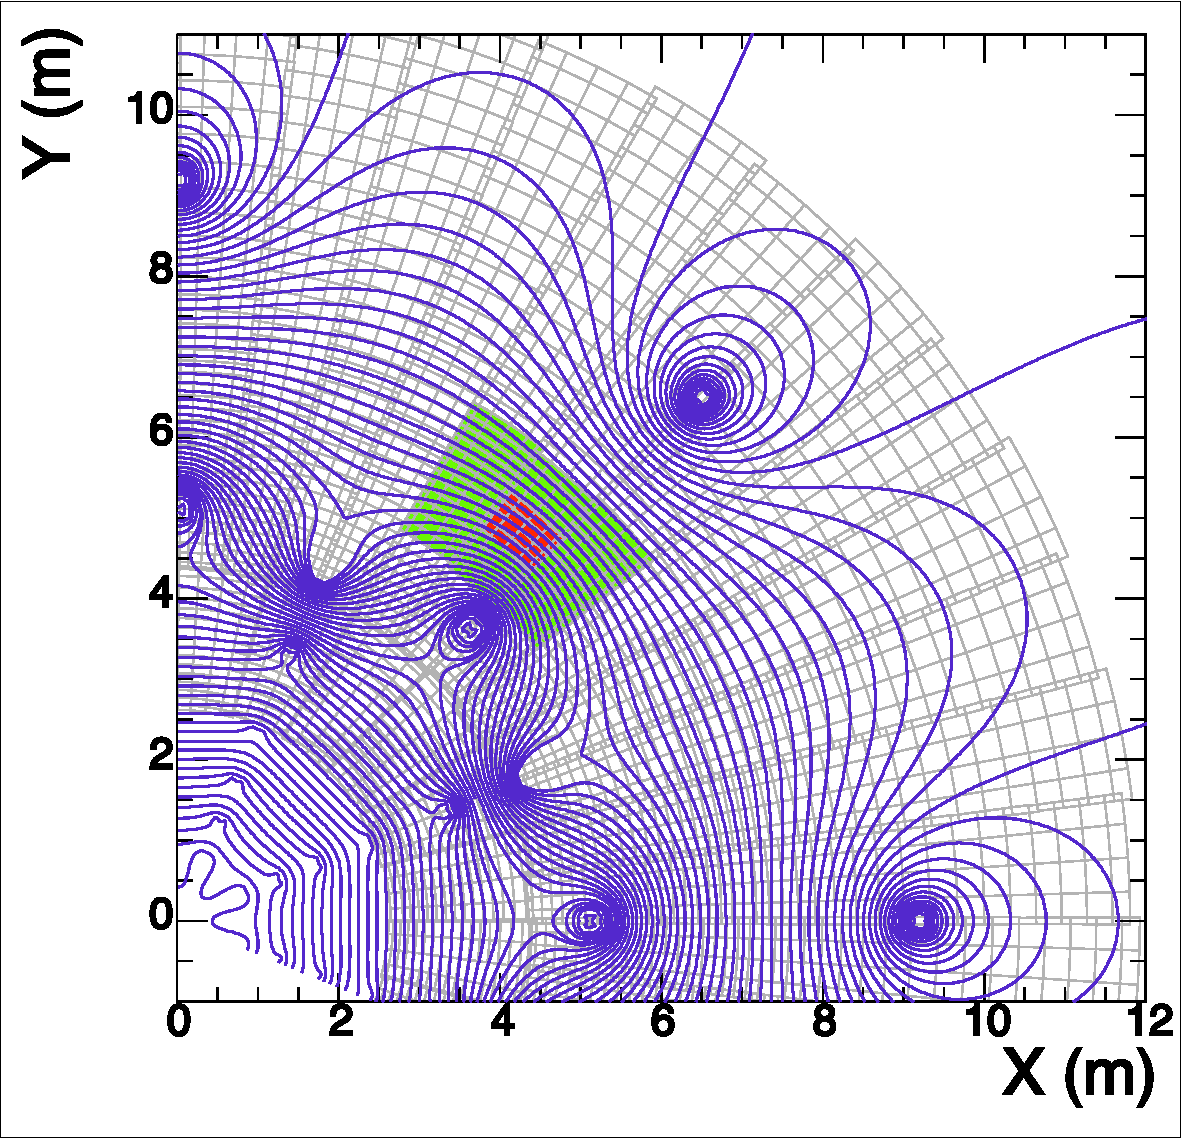
\includegraphics[clip, width=9cm]{fig/4/c1_withMag.pdf}
  \caption{磁場構造を考慮するための学習領域の分け方。赤色の領域に対するトレーニングを行う際には緑色で囲まれたの領域のデータを使用する。}
  \label{fig:Mag}
\end{figure}

\subsubsection{ミューオン情報の選別}
次に各RoIにおけるヒットマップを作成し学習に使用するミューオンの選別を行う。作成したヒットマップには孤立しているマスが存在する。
これは偶発的にミューオンがヒットしたことや多重散乱の影響によるもので、このままトレーニングに用いると本来$p_{\rm{T}}$を判定する必要のないマスまで学習してしまい、トリガーレートの増加に繋がってしまう。
そのため、以下に説明する手順に沿ってヒットマップを用いたミューオンの選別行う。
図~\ref{fig:hitmapcleaner}にヒットマップクリーナを作用させた場合の例を示す。
\begin{enumerate}
   \item エントリー数が 3 以下のマスは削除する。これは、偶発的にミューオンがヒットしたマスを削除することを目的とする。
   \item あるマスに隣接する周囲の8マスのうち、ミューオンがヒットしたマスが2マス以下であるとき、削除する。これは、孤立したミューオンのヒットを削除することを目的としている。
\end{enumerate}


\begin{figure}[tb]
  \centering
  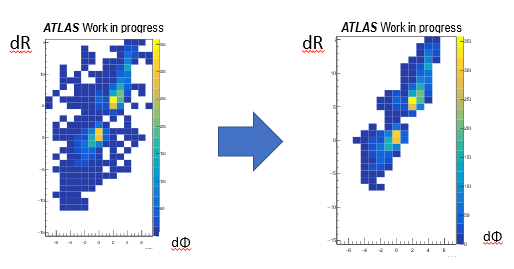
\includegraphics[clip, width=14cm]{fig/4/cleaner.png}
  \caption{ヒットマップクリーナーをかけた前後のミューオンヒットマップの例}
  \label{fig:hitmapcleaner}
\end{figure}


\subsection{機械学習モデルの設計方法とトレーニング}
本節では飛跡の曲がり具合と TGC$\_$BW のヒット情報からミューオンの横方向運動量 $p_{\rm{T}}$を出力させる機械学習モデルの設計について述べる。

\subsubsection{機械学習モデルの設計}
本研究において、機械学習モデルの構築にはGoogle社によって開発された機械学習に用いるためのオープンソースのフレームワークであるTensorFlow~\cite{article:TensorFlow}とニューラルネットワークライブラリであるKeras~\cite{article:keras}を用いた。

本研究で使用する機械学習モデルは、4つの入力変数を持つ入力層、5つの隠れ層、$p_{\rm{T}}$の値を出力する1つの出力層となるような、回帰分析を行う全結合型MLPモデルを構築する。
図~\ref{fig:MLP_overview}に機械学習モデルの概要図を示す。
MLPの各隠れ層は以下の表\ref{table:hibben}に示す要素から構成される。
\begin{enumerate}\label{table:hibben}
   \item Dence layer:前の層からのすべての出力の線形結合を入力としたパーセプトロンの層。1 つの層に存在するパーセプトロンの数をノード数と呼ぶ。
   \item Batch normalization layer:入力に対し正規化を行う層。
   \item Dropout unit:学習中にランダムに選ばれたノードの一定割合をゼロにする操作。過学習の抑制のために用いられ、ドロップアウトする割合はハイパーパラメータとして設定する。
   \item Activation unit:活性化関数を設定する層。
   %\caption{隠れ層を構成する要素。}
\end{enumerate}
出力層には ReLU 関数を活性化関数として使用する。これは、目的とする出力の $p_{\rm{T}}$の値が必ず正の値を取るためである。
誤差逆伝搬法にはRMSpropを用いて勾配降下法を行っている。

\subsubsection{ハイパーパラメータ}
隠れ層の数、ノード数、ドロップアウト率、損失関数、学習率の 5 個のハイパーパラメータを表\ref{table:hyper}のように変化させることで評価を行い最適なモデルを選択した。評価にはPreferred Networks社が開発したハイパーパラメータの最適化を自動で行うフレームワークである Optuna \cite{article:optuna}を使用した。
\begin{enumerate}\label{table:hyper}
   \item 隠れ層の数:3層 から 6層
   \item ノード数:128, 256, 512, 1024
   \item ドロップアウト率:0.01, 0.02, 0.03, 0.04, 0.05
   \item 活性化関数:Sigmoid 関数、ReLU 関数
   \item 学習率:0.01, 0.001, 0.0001
   %\caption{変化させるハイパーパラメータの一覧。}
\end{enumerate}
評価を行った結果、いくつかの組み合わせで同等の性能が得られることがわかった。これらのうち、学習可能なパラメータの数が最も少ないネットワークが選ばれた。パラメータとその値は、ドロップアウト率 0.05、活性化関数 ReLU、学習率 0.001, そして、5つの隠れ層と [256, 256, 256, 256, 256] のノード数を選択する。
また、epochs~(トレーニングを繰り返す回数)を50、batch$\_$size~(トレーニングデータを分割したサブセットの1個当たりのイベント数)を3000とした。

\begin{figure}[tb]
  \centering
  %\rule{8cm}{6cm}
  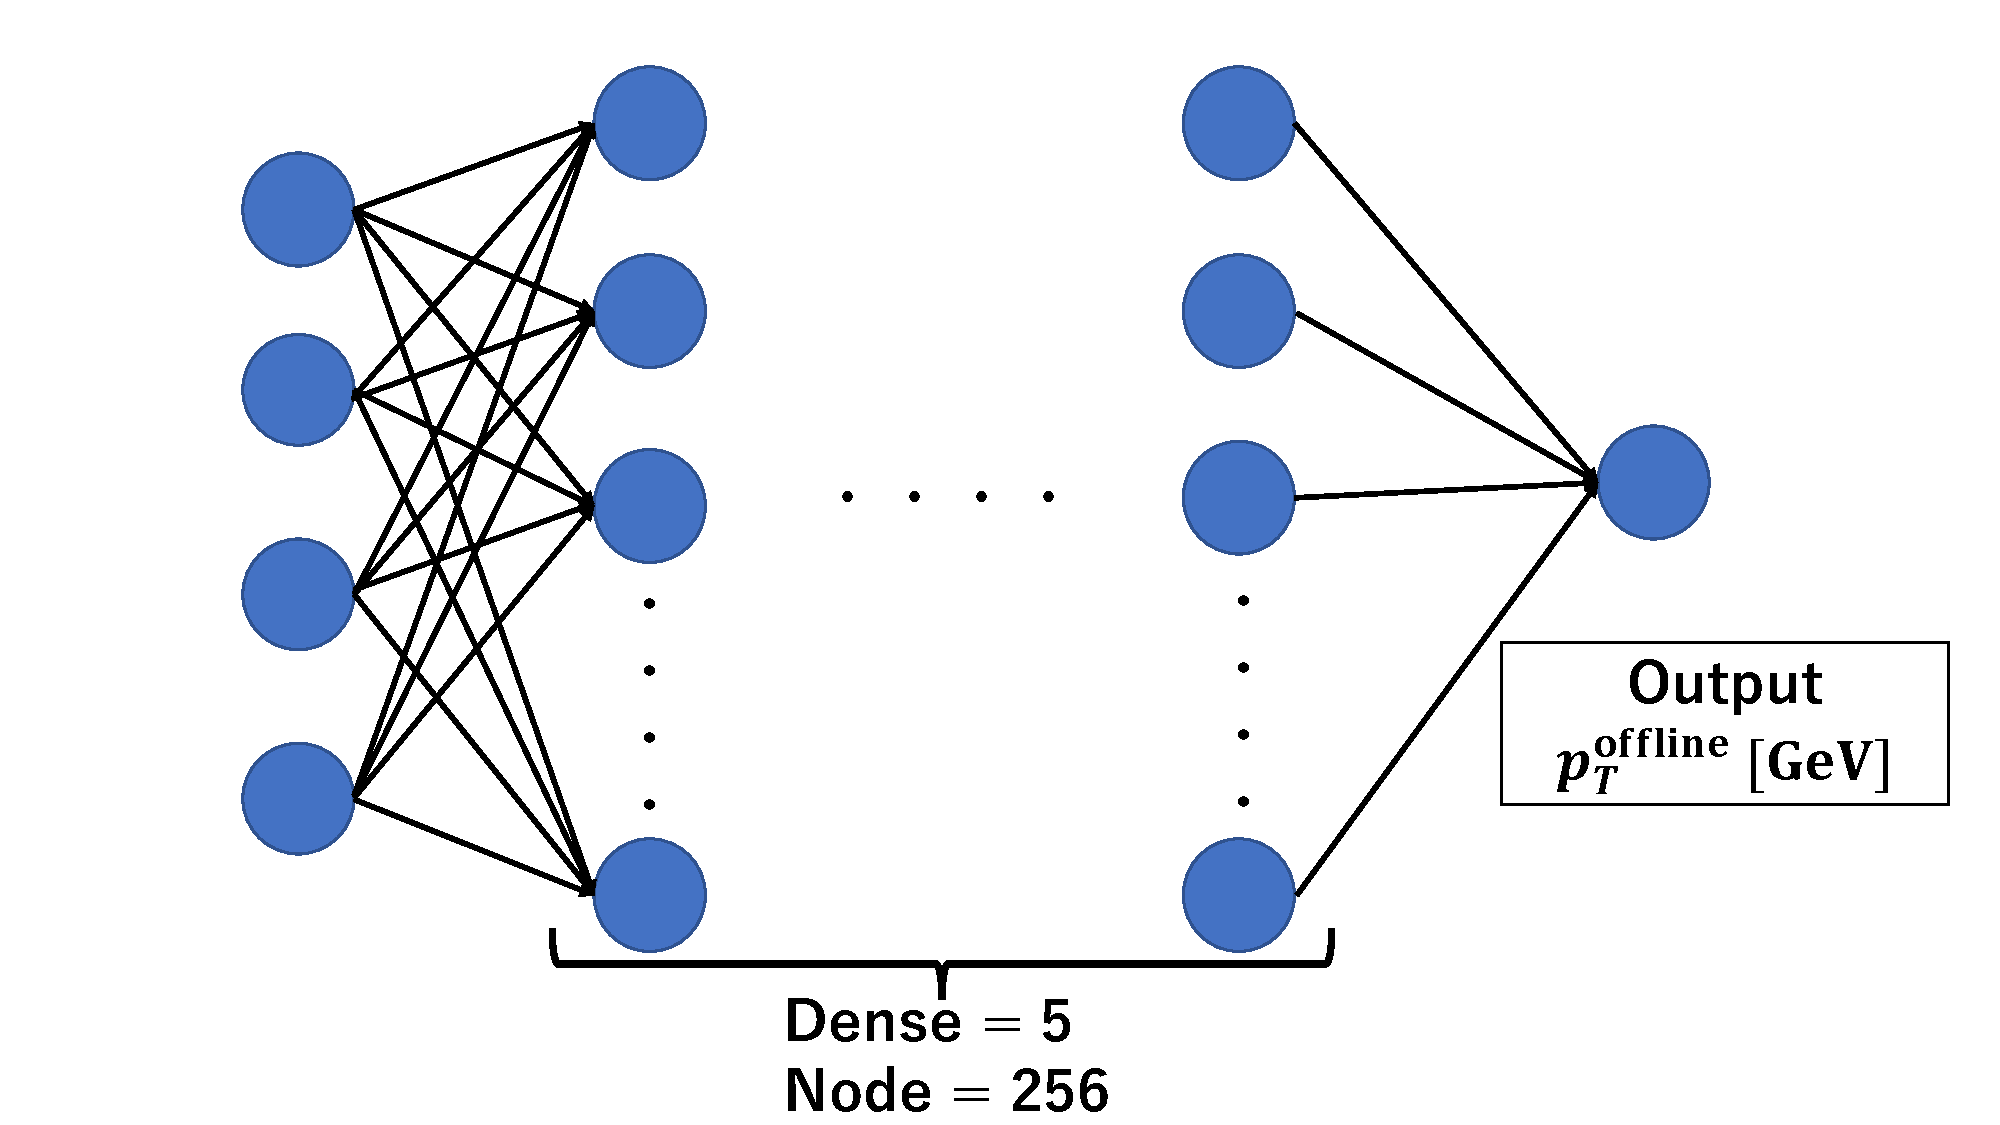
\includegraphics[clip, width=12cm]{fig/4/MLP_2.pdf}
  \caption{機械学習モデルの概要図。4つの入力、各層に256個のノードを持つ5つの隠れ層、$p_{\rm{T}}^{\rm{offline}}$を出力とする全結合型MLPを構築する。}
  \label{fig:MLP_overview}
\end{figure}


\subsubsection{トレーニング}
\ref{事前処理}節で述べたように、シミュレーション用のCWを作成するための機械学習のトレーニングには、シングルミューオンのシミュレーションサンプルを使用し、実際の測定用のCWを作成するための機械学習のトレーニングには、2018年Run-2で収集されたデータを使用する。この実際のデータ及びシミュレーションデータに対して事前処理を行ったデータを入力データとする。教師データとしてはそれぞれのデータでオフライン再構成されたミューオンの$p_{\rm{T}}$を利用する。
トレーニングデータの総数は、シミュレーションデータが500万イベント、2018年Run-2データが約1億イベントである。
図~\ref{Inputdata}にトレーニングに用いたミューオンの$p_{\rm{T}}$分布を示す。
\begin{figure}
    %\centering
    \begin{tabular}{cc}
    \centering
    \begin{minipage}[b]{0.45\hsize}%
        \centering
        \hspace*{-1cm}
        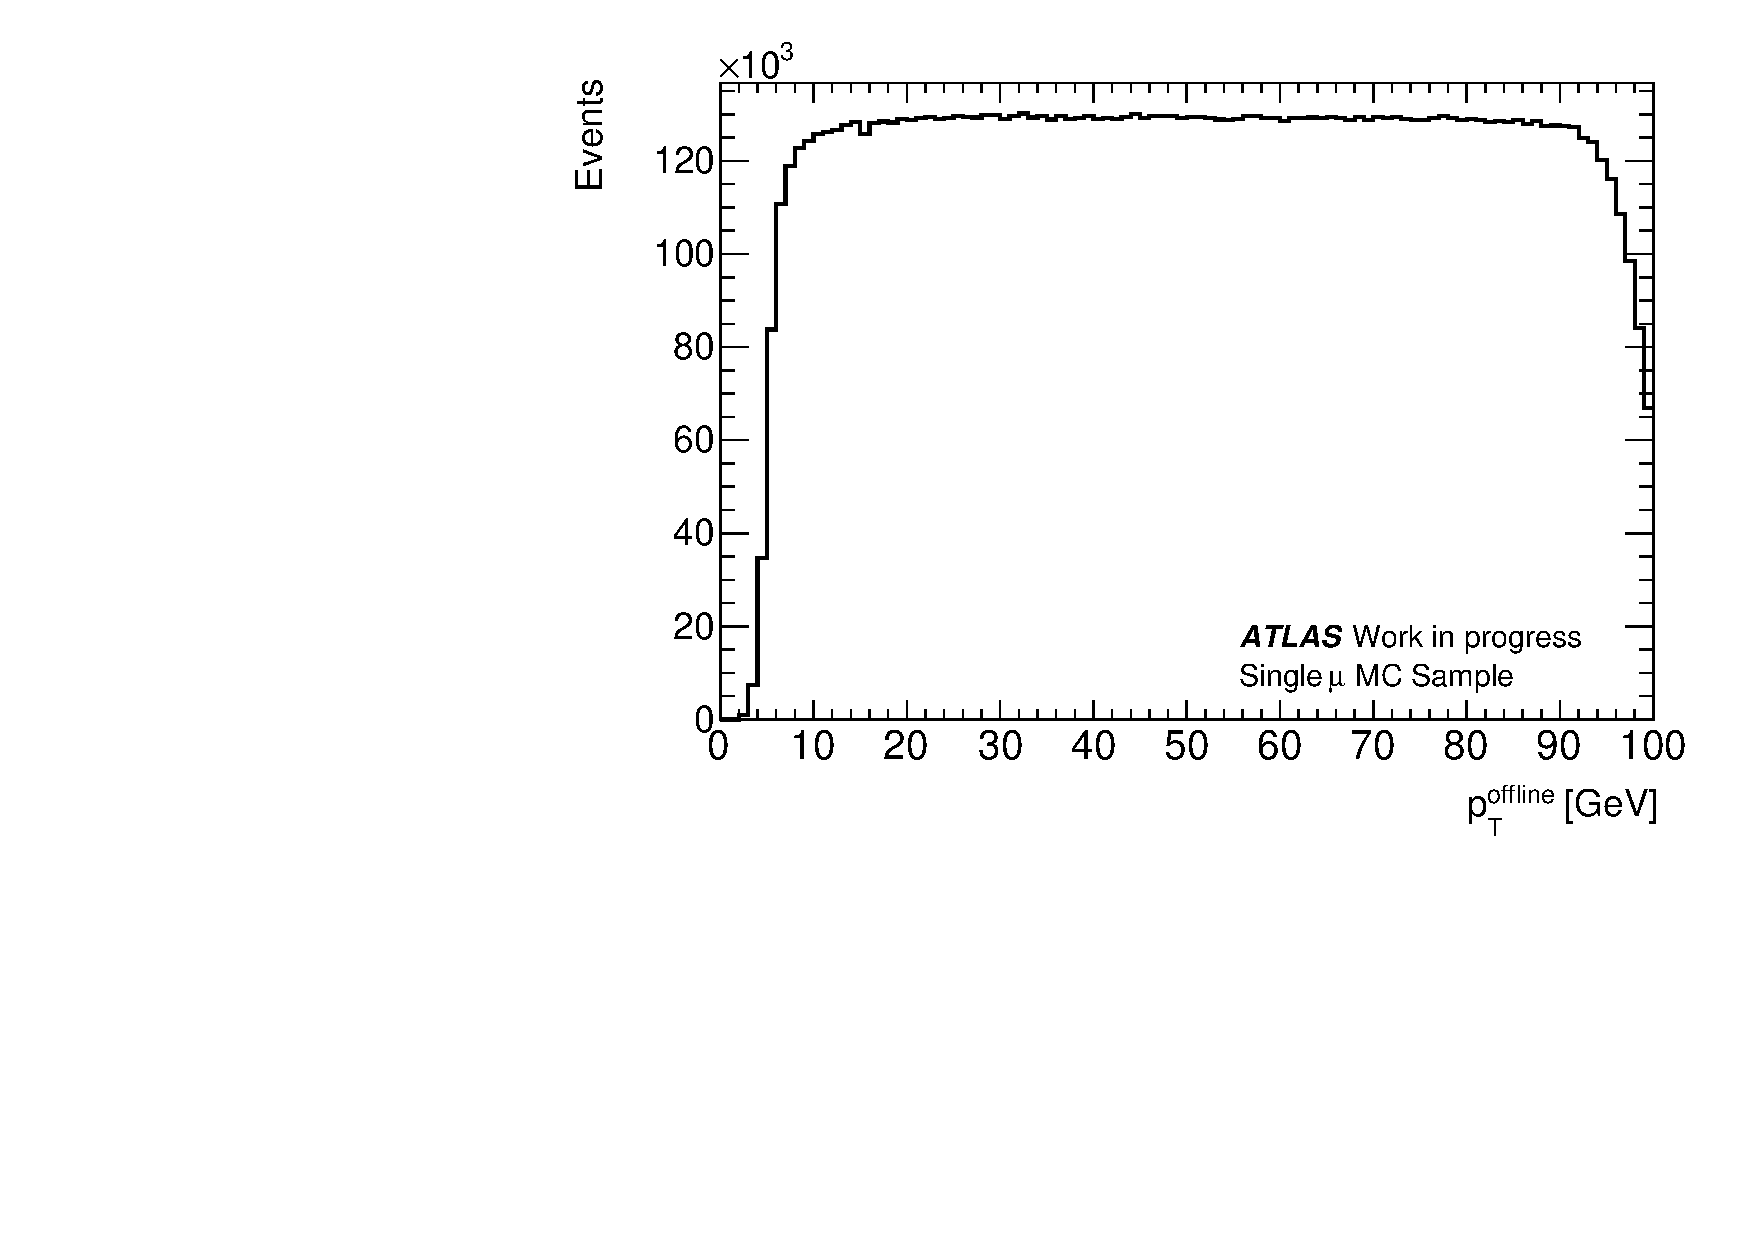
\includegraphics[clip, width=7cm]{fig/4/MC_input_pt100.pdf}
        %\vspace{5pt}
        \subcaption{}
        \label{MC_input}
    \end{minipage}%
    %\hfill
    \begin{minipage}[b]{0.6\hsize}%
        \centering
        \hspace*{-1cm}
        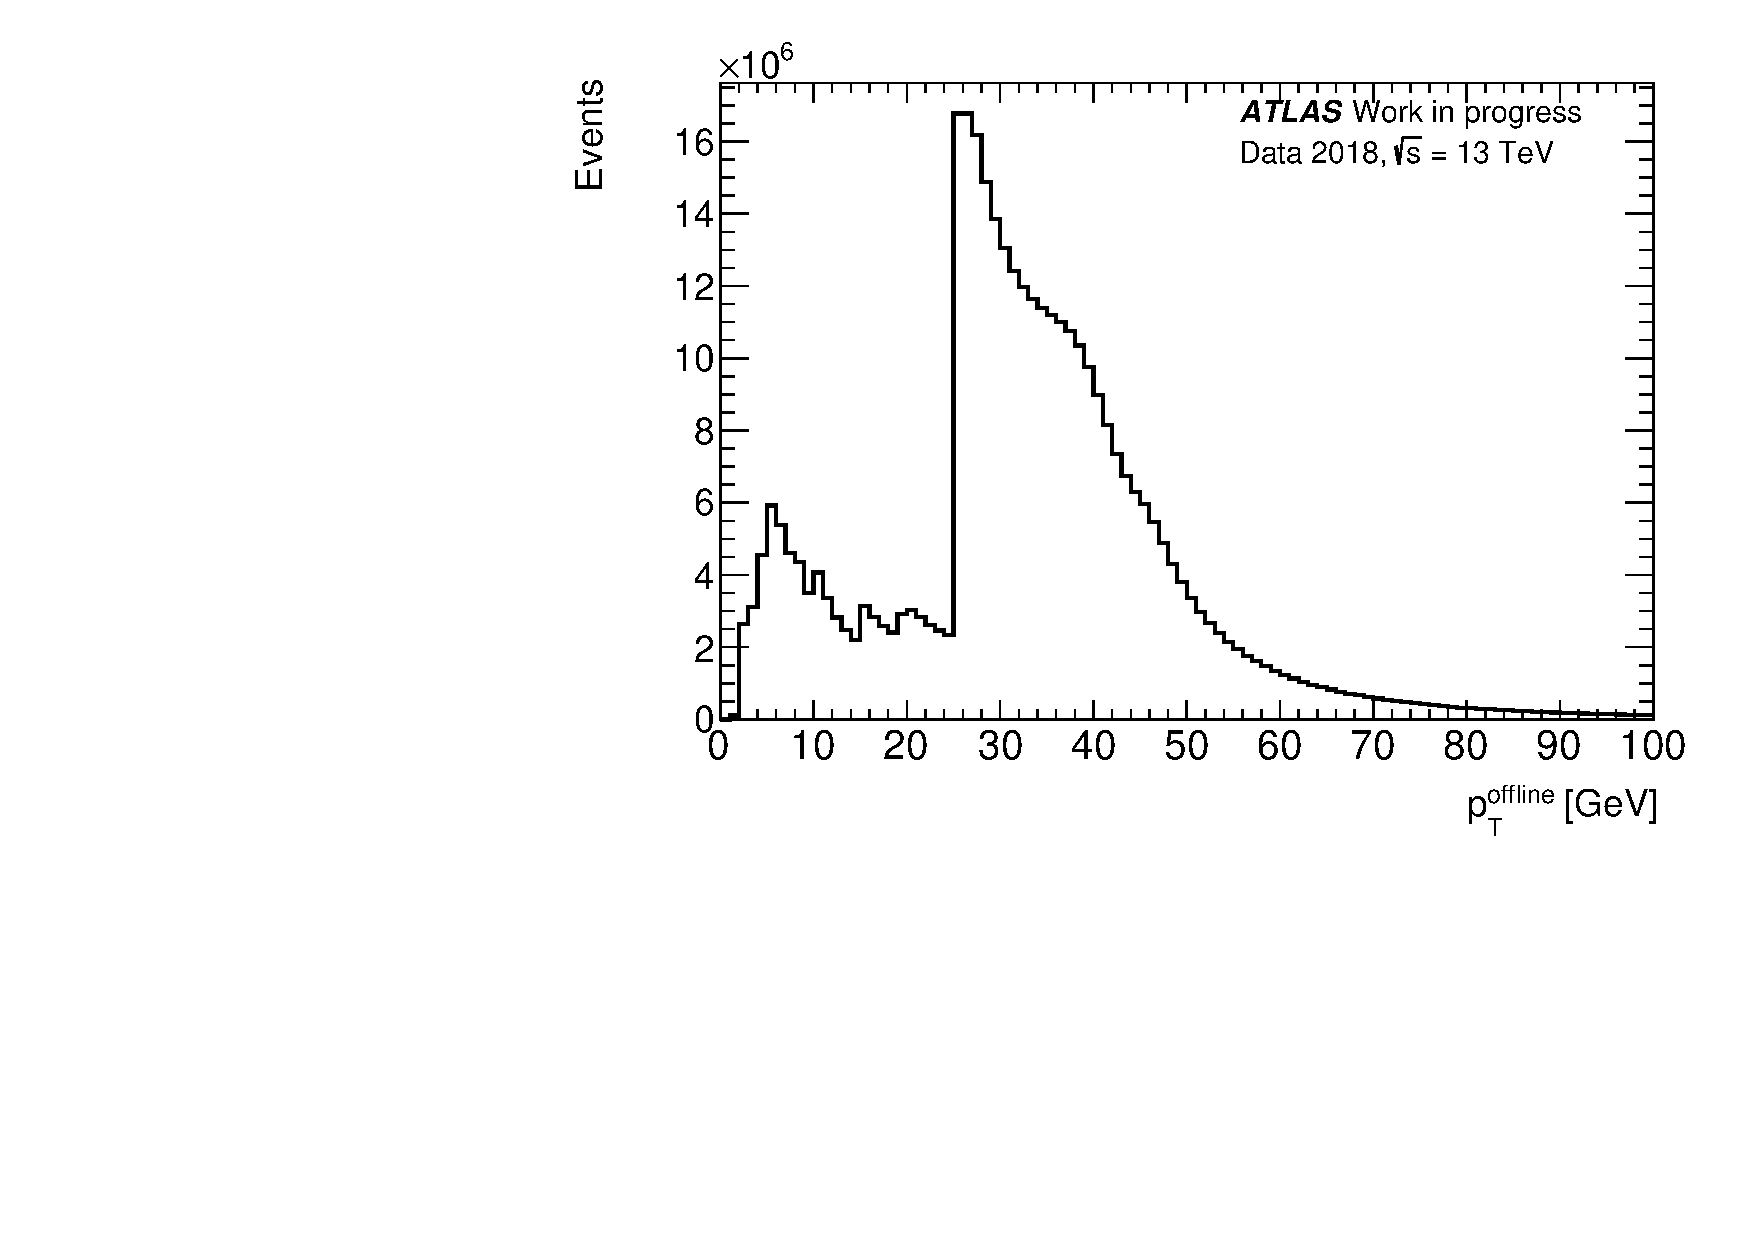
\includegraphics[clip, width=7cm]{fig/4/Data_input_pt.pdf}
        %\vspace{5pt}
        \subcaption{}
        \label{Data_input}
    \end{minipage}%
    \end{tabular}
    \caption{トレーニングに用いたミューオンの$p_{\rm{T}}$分布。(a):シングルミューオンのシミュレーションサンプル。(b):2018年Run-2のデータ。}
    \label{Inputdata}
\end{figure}

%図~\ref{fig:epoch}に機械学習モデルをトレーニングした際のepochに対する出力と教師データの平均二乗誤差の推移を示す。全てのモデルにおいてvalidationデータの平均二乗誤差は十分に収束している事が見て取れる。

%\begin{figure}[tb]
%  \centering
%  %\rule{8cm}{6cm}
%  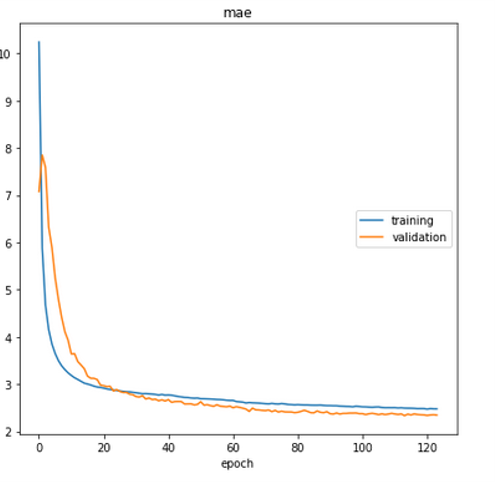
\includegraphics[clip, width=7cm]{fig/4/epoch2.png}
%  \caption{機械学習モデルをトレーニングした際の epoch に対する平均二乗誤差の推移。}
%  \label{fig:epoch}
%\end{figure}


\newpage
\subsubsection{機械学習モデルの性能評価}
本節では、機械学習モデルについての評価を行う。
新たに500万イベントのシングルミューオンのシミュレーションデータ作成し評価に用いて、MLPで予測した$p_{\rm{T}}^{Pred}$とオフライン再構成された正解値 $p_{\rm{T}}^{True}$の比較を行った結果を図~\ref{fig:zannsa_25_MC}に示す。
また、2018年Run-2で収集したデータを用いて、MLP で予測した$p_{\rm{T}}^{pred}$と正解値 $p_{\rm{T}}^true$の残差分布の比較を行った結果を図~\ref{fig:zannsa_25_Data}に示す。
さらに、ある$p_{\rm{T}}^{True}$に対して、$p_{\rm{T}}^{Pred}$の分布をガウシアンフィットした場合のmean値の分布を図~\ref{fig:Gausmu}に示す。シミュレーション用と実際の測定用のそれぞれにおいて、$p_{\rm{T}}^{True}$に対して機械学習の予測値はほぼ線形である事が見て取れ、ミューオンの$p_{\rm{T}}^{True}$の予測が行えていることが確認できる。
\begin{figure}
    %\centering
    \begin{tabular}{cc}
    \centering
    \begin{minipage}[b]{0.45\hsize}%
        \centering
        \hspace*{-1cm}
        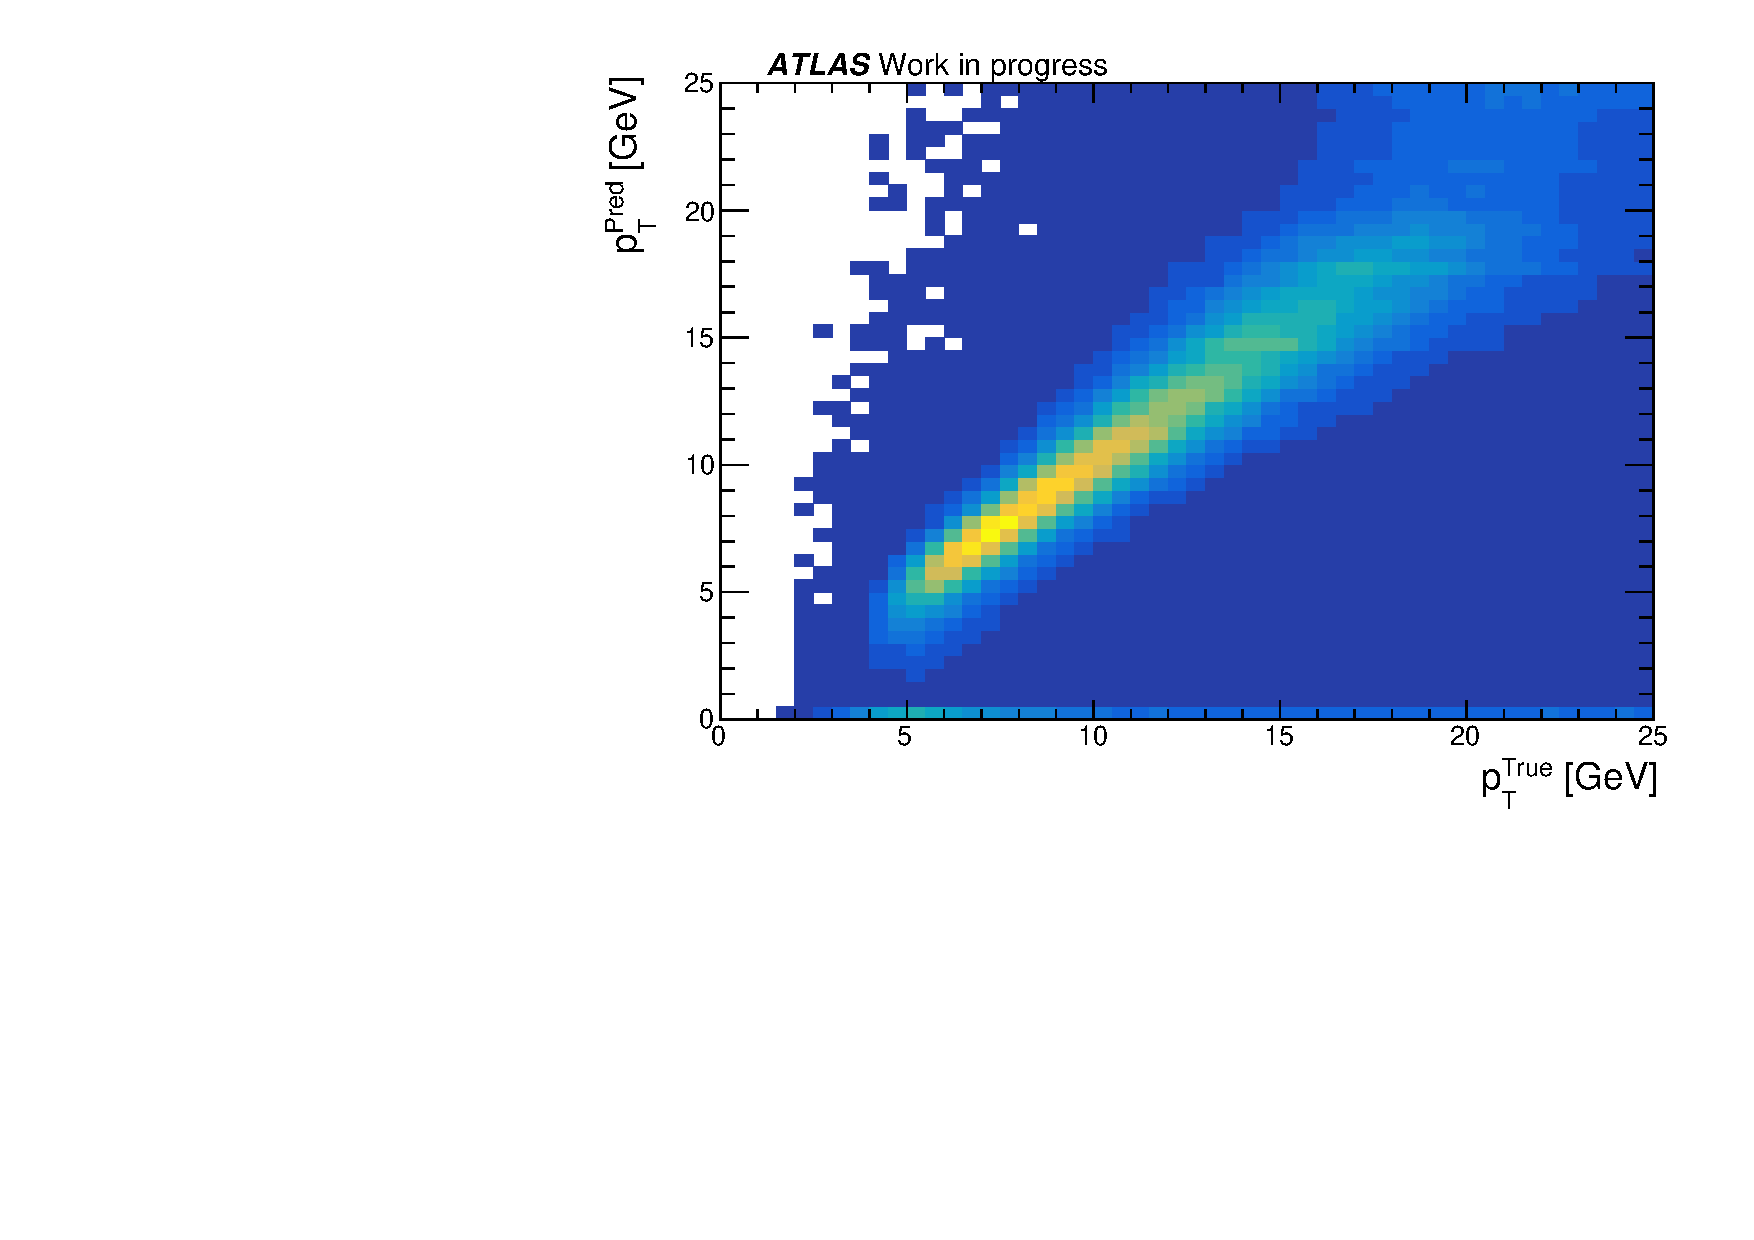
\includegraphics[clip, width=8cm]{fig/4/MC_pred_true_25.pdf}
        %\vspace{5pt}
        \subcaption{}
        \label{fig:zannsa_25_MC}
    \end{minipage}%
    %\hfill
    \begin{minipage}[b]{0.7\hsize}%
        \centering
        %\hspace*{-cm}
        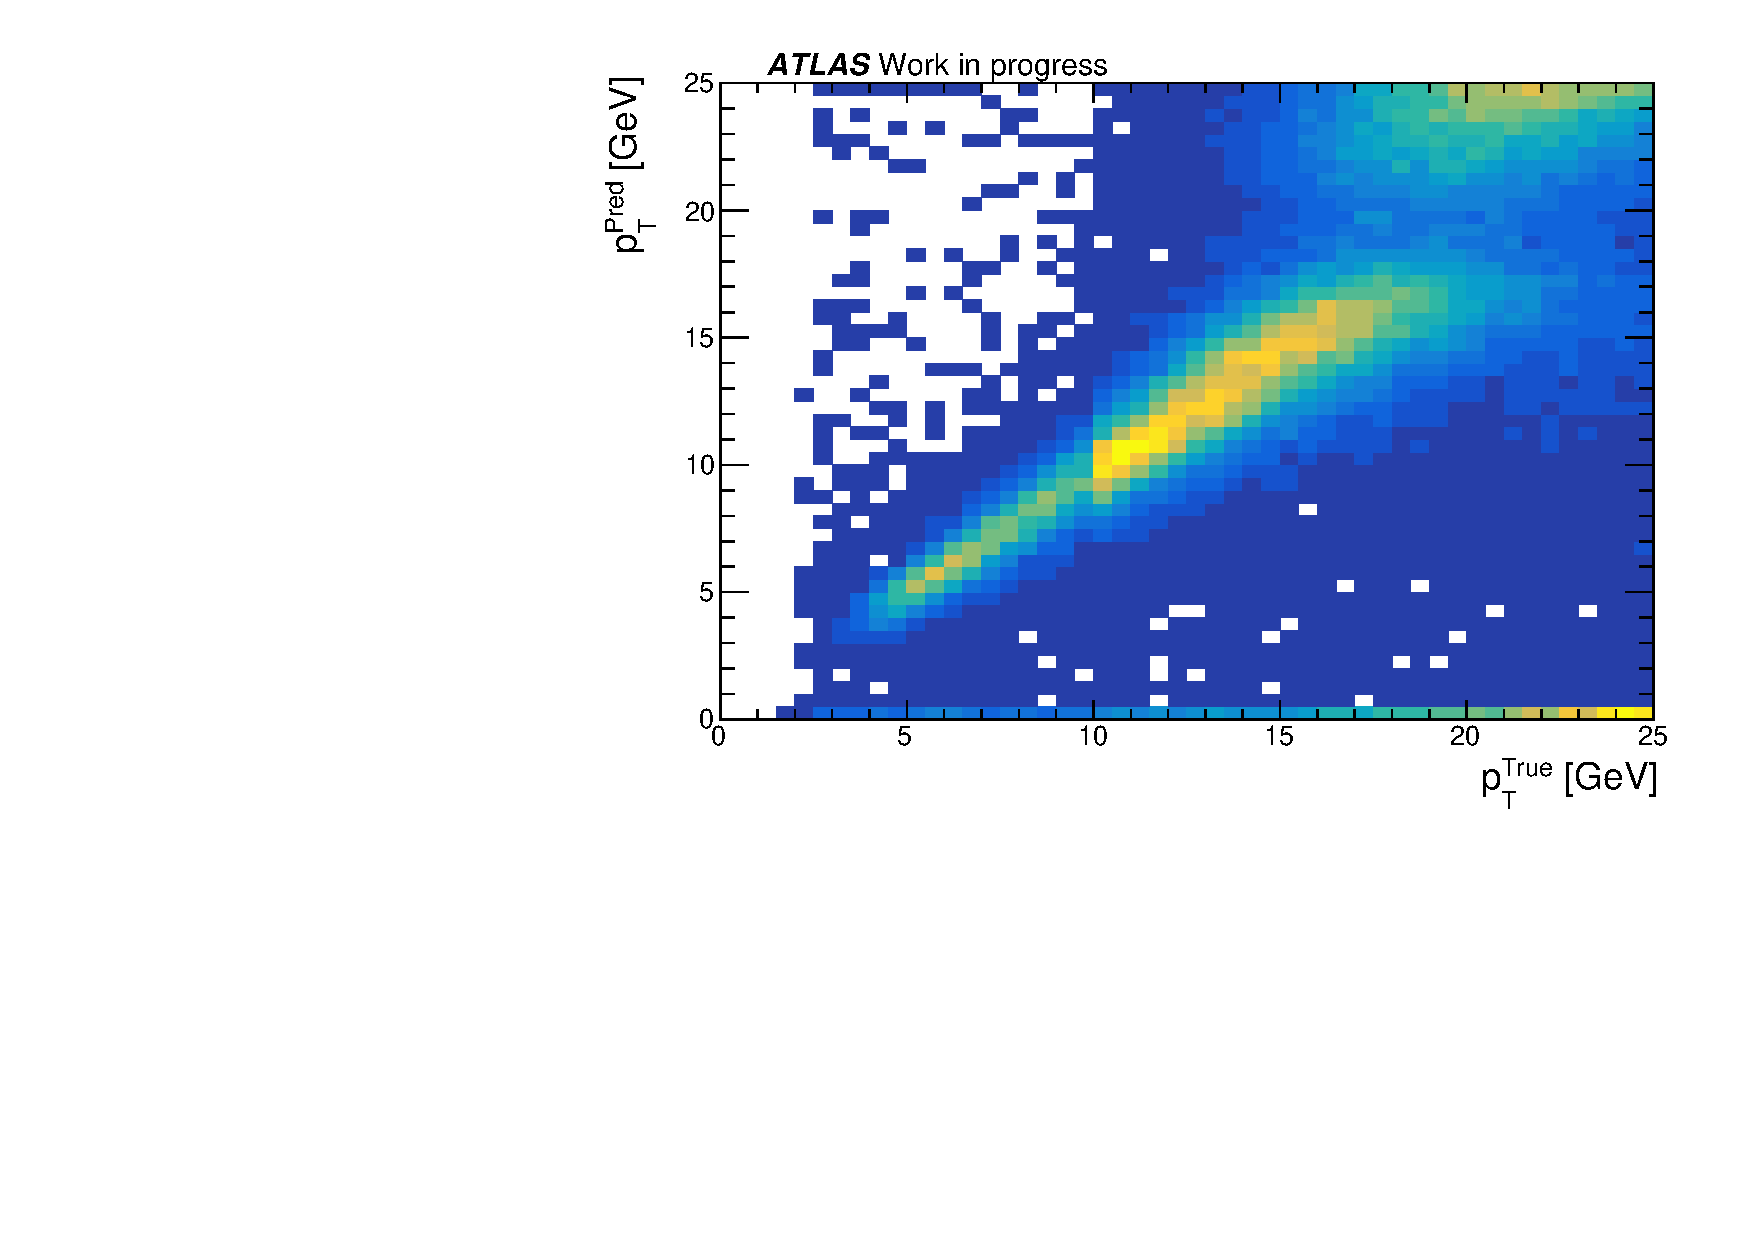
\includegraphics[clip, width=8cm]{fig/4/pred_true_25.pdf}
        %\vspace{5pt}
        \subcaption{}
        \label{fig:zannsa_25_Data}
    \end{minipage}%
    \end{tabular}
    \caption{MLPの$p_{\rm{T}}^{True}$に対する$p_{\rm{T}}^{Pred}$の分布。ト(a):2018年Run-2のデータ。(b):シミュレーションデータを用いてトレーニングを行ったMLP。(b):2018年Run-2のデータを用いてトレーニングを行ったMLP。}
    \label{25}
\end{figure}

%\begin{figure}[tb]
%  \centering
%  %\rule{8cm}{6cm}
%  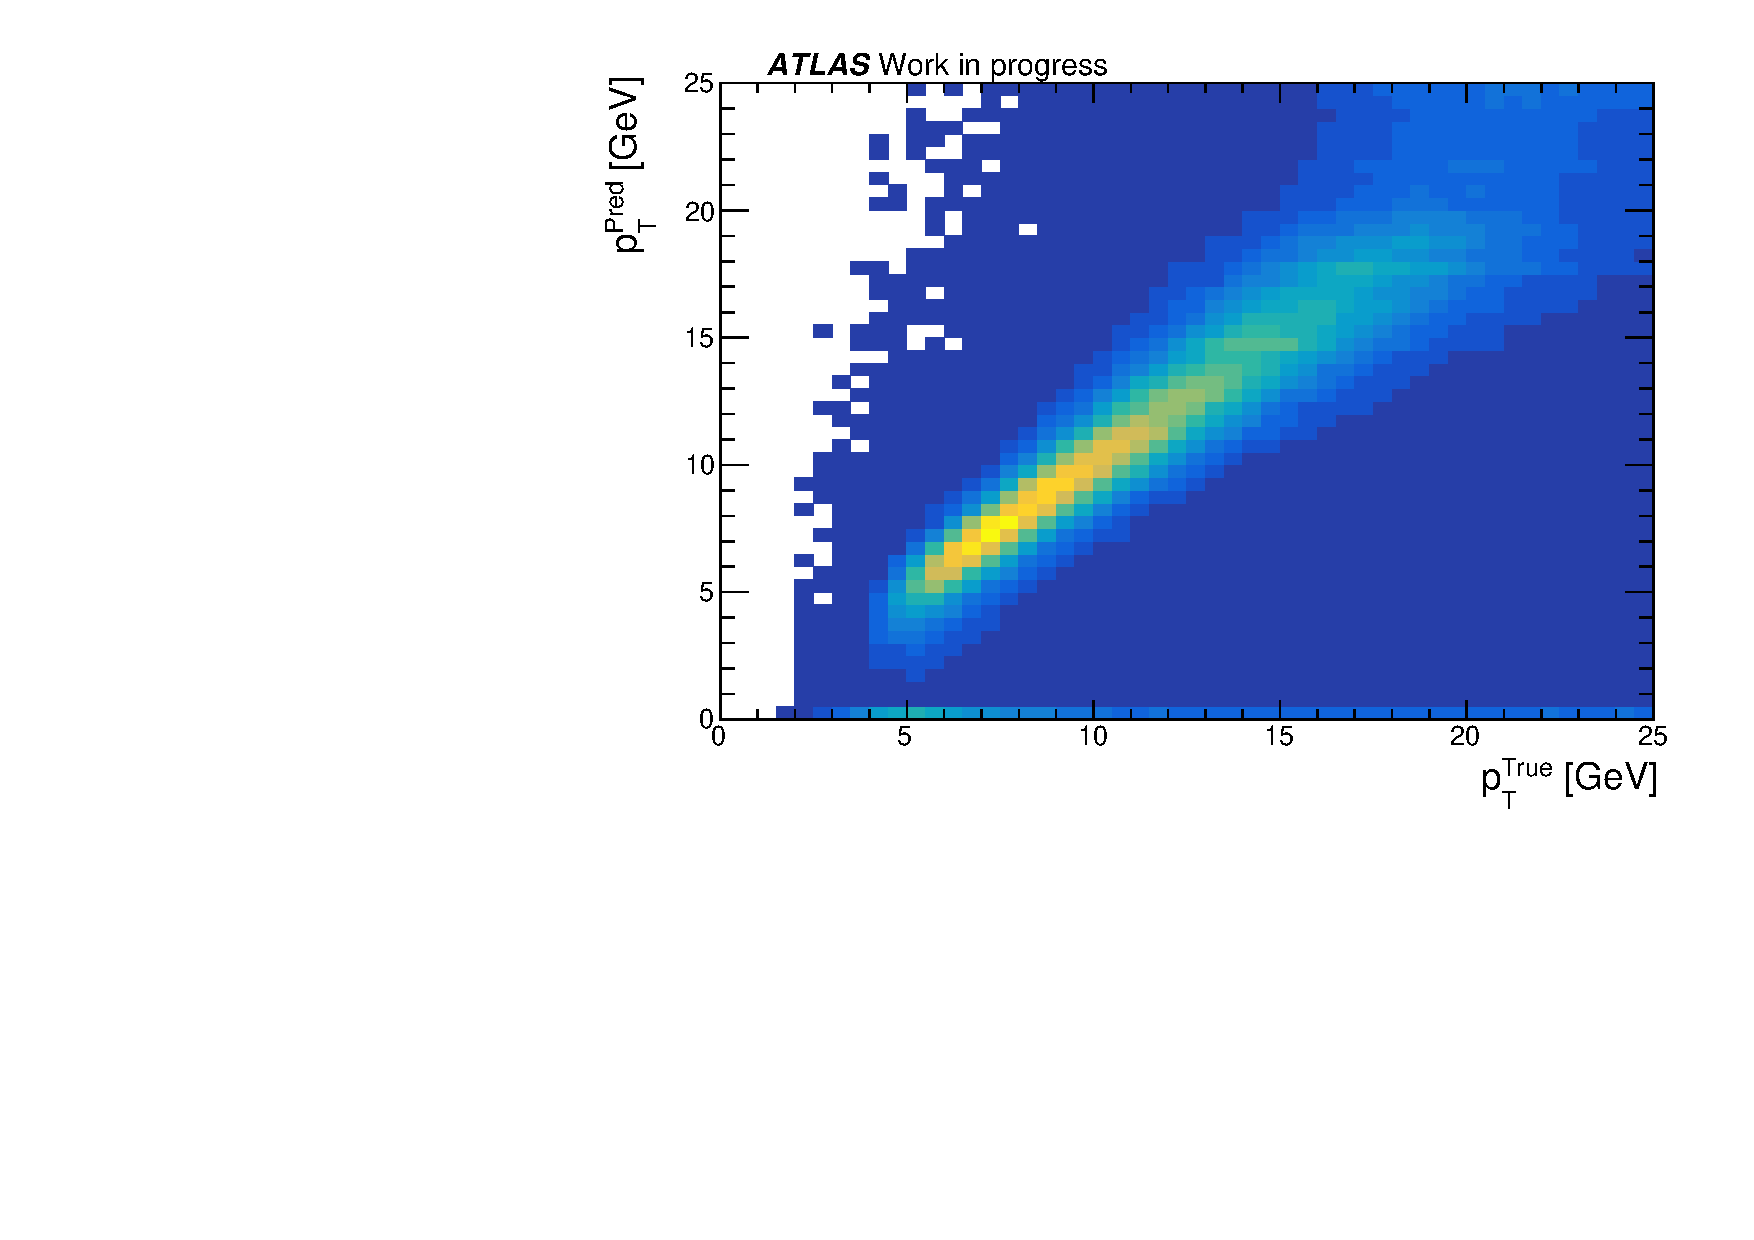
\includegraphics[clip, width=10cm]{fig/4/MC_pred_true_25.pdf}
%  \caption{シミュレーションデータを用いてトレーニングを行ったMLPの$p_{\rm{T}}^{True}$に対する$p_{\rm{T}}^{Pred}$の分布。評価にはシングルミューオンのシミュレーションデータを用いた。}
%  \label{fig:zannsa_25_MC}
%\end{figure}



\begin{figure}
    %\centering
    \begin{tabular}{cc}
    \centering
    \begin{minipage}[b]{0.45\hsize}%
        \centering
        \hspace*{-1cm}
        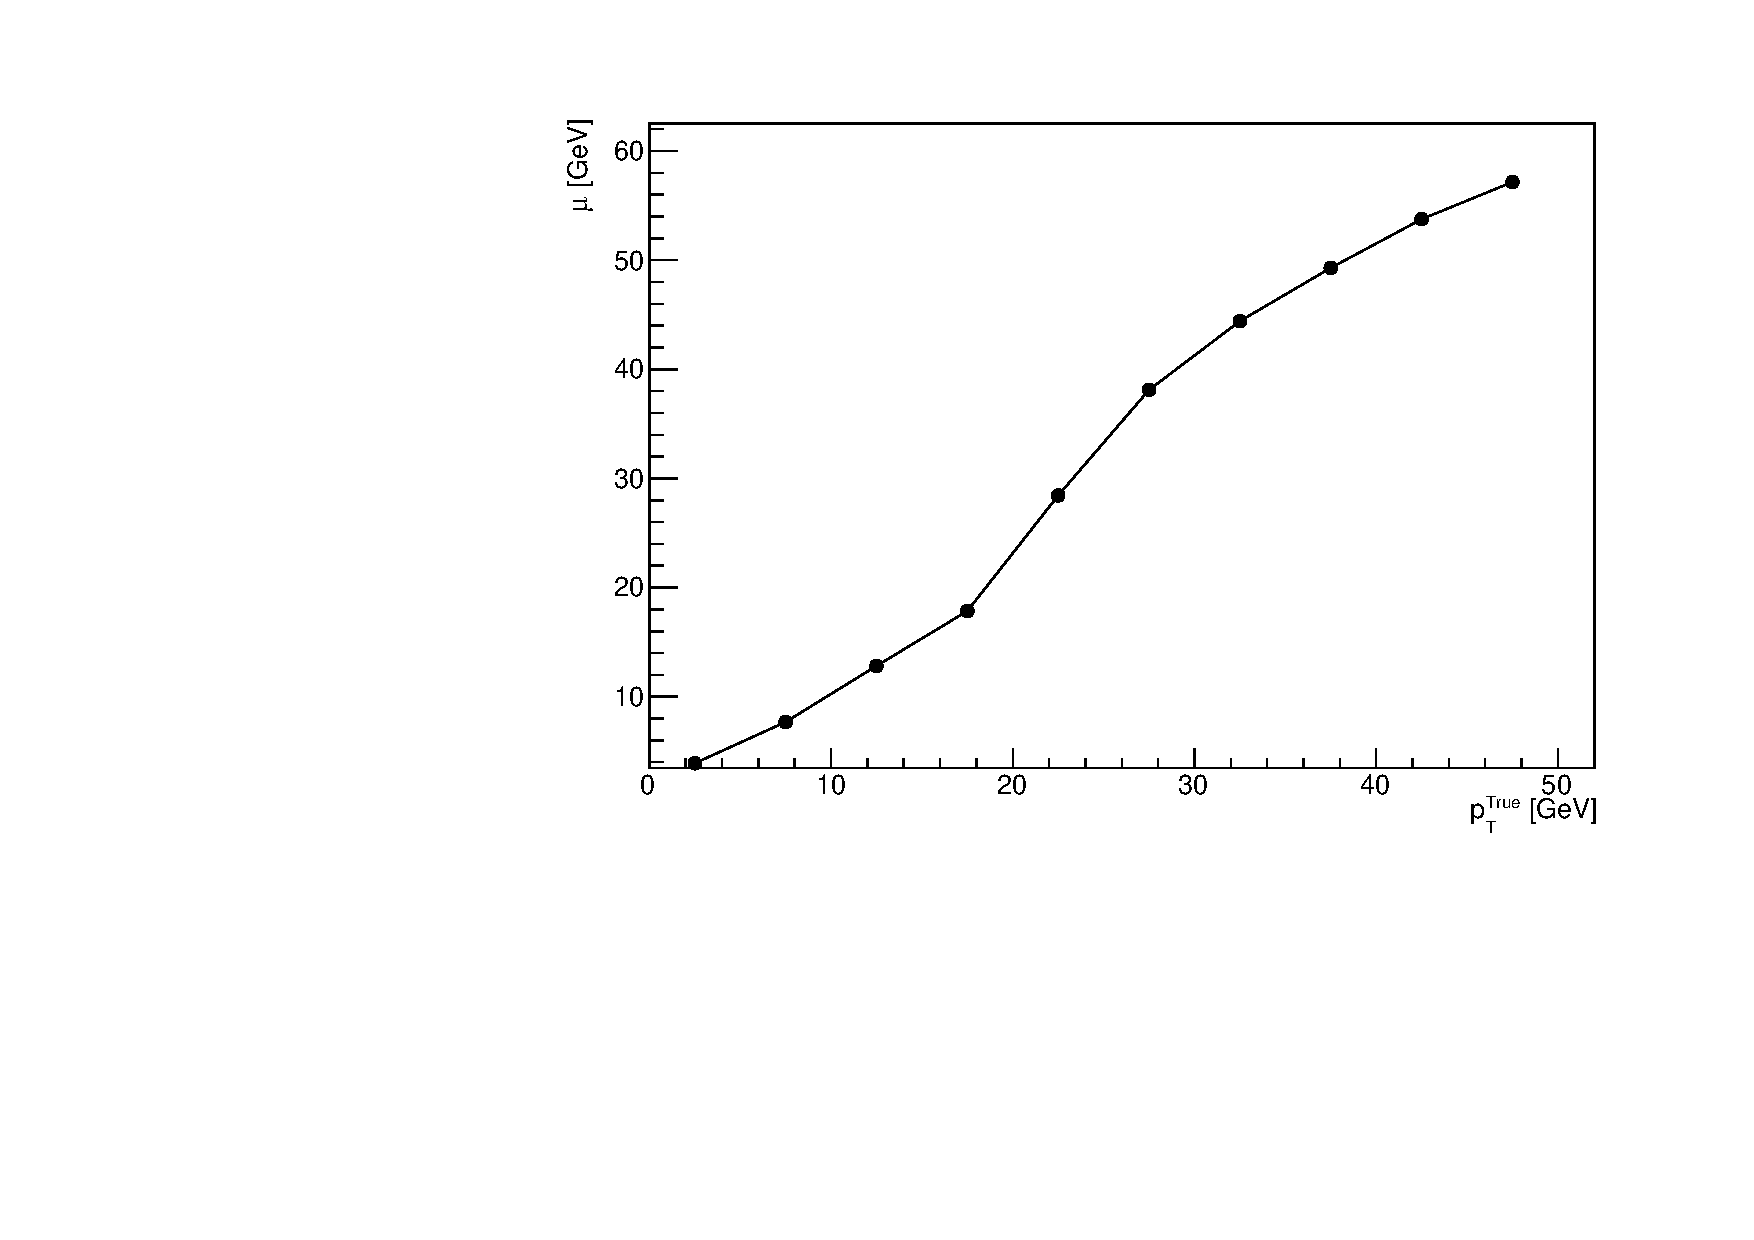
\includegraphics[clip, width=8cm]{fig/4/tp_Gausmean_MC.pdf}
        %\vspace{5pt}
        \subcaption{}
        \label{}
    \end{minipage}%
    %\hfill
    \begin{minipage}[b]{0.7\hsize}%
        \centering
        %\hspace*{-cm}
        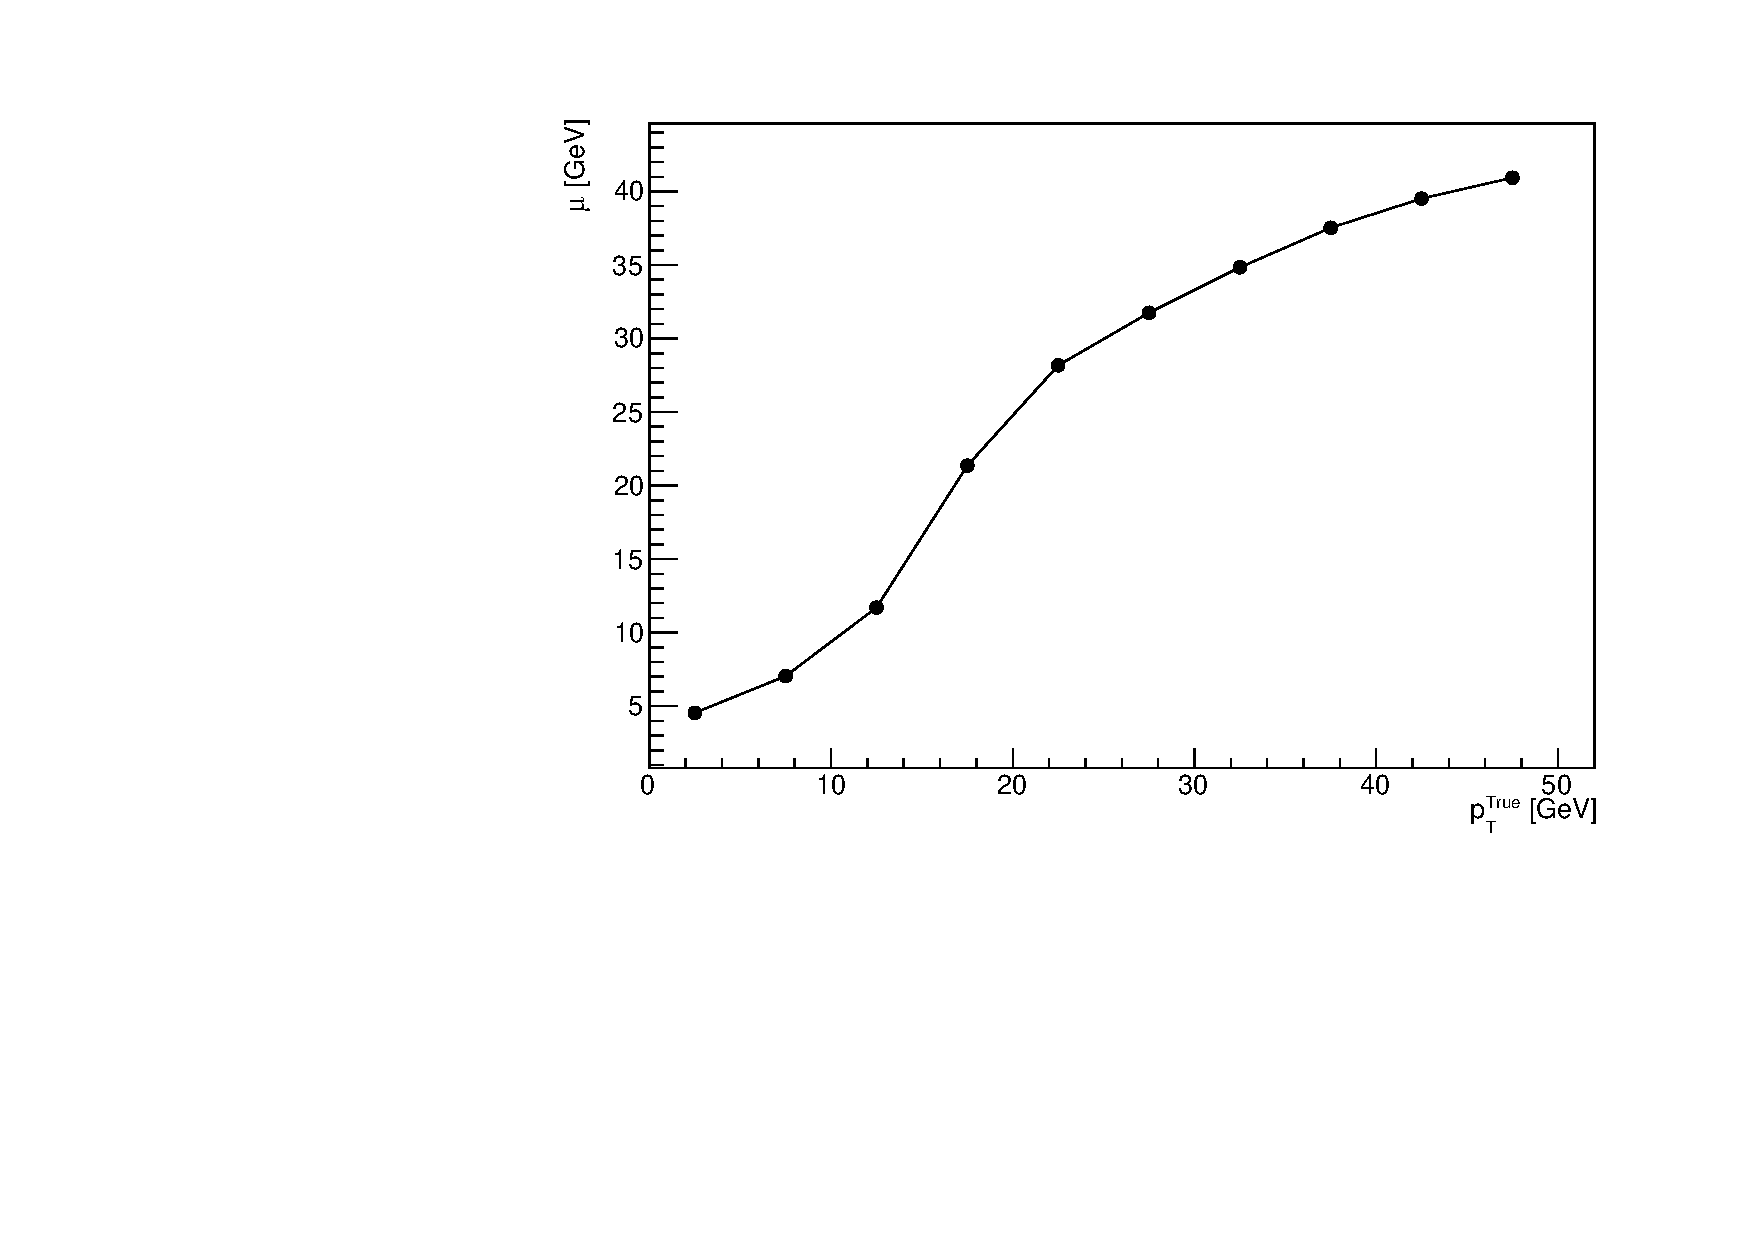
\includegraphics[clip, width=8cm]{fig/4/tp_Gausmean_Data.pdf}
        %\vspace{5pt}
        \subcaption{}
        \label{MC_input}
    \end{minipage}%
    \end{tabular}
    \caption{ある$p_{\rm{T}}^{True}$に対して、$p_{\rm{T}}^{Pred}$の分布をガウシアンフィットした場合のmean値の分布。(b):シミュレーションデータを用いてトレーニングを行ったMLP。(b):2018年Run-2のデータを用いてトレーニングを行ったMLP。}
    \label{fig:Gausmu}
\end{figure}


%\begin{figure}[tb]
%  \centering
%  %\rule{8cm}{6cm}
%  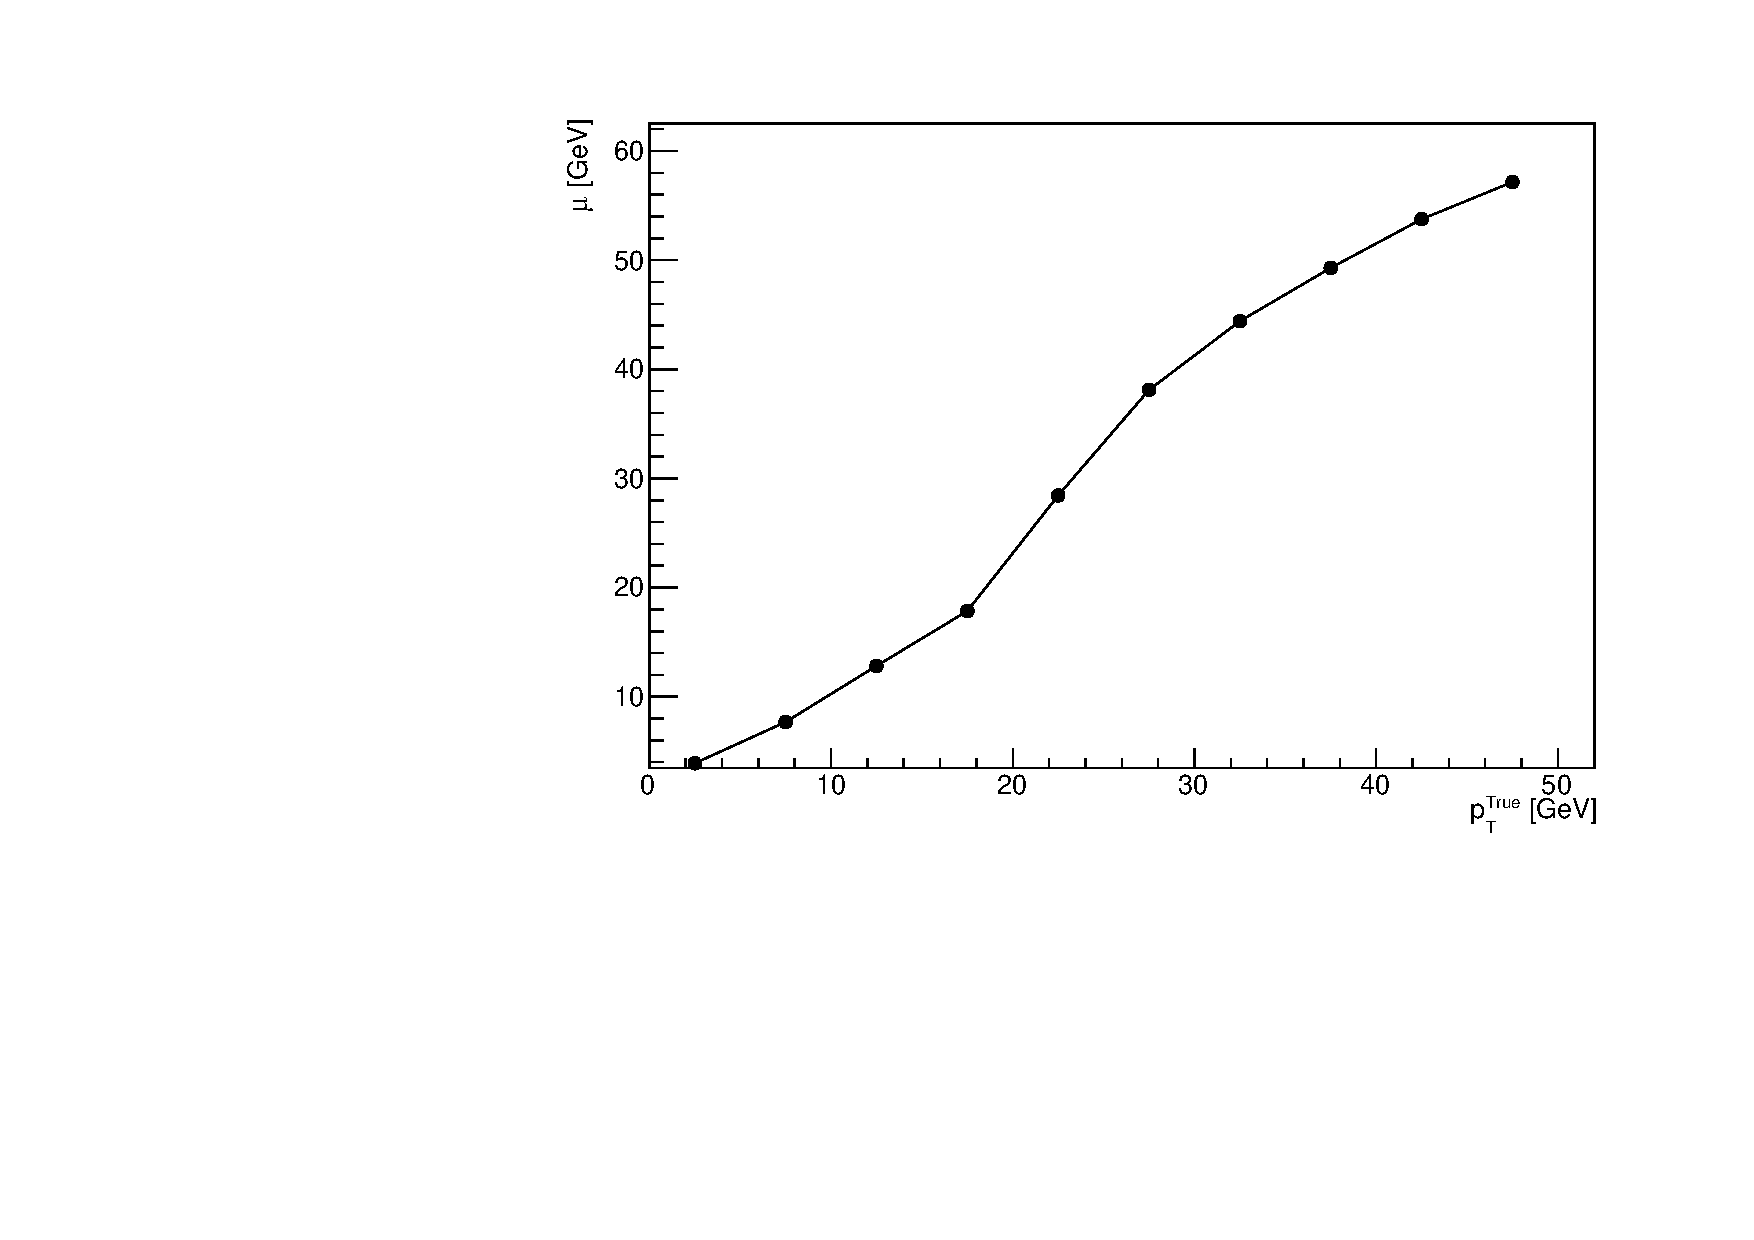
\includegraphics[clip, width=10cm]{fig/4/tp_Gausmean_MC.pdf}
%  \caption{ある$p_{\rm{T}}^{True}$に対して、$p_{\rm{T}}^{Pred}$の分布をガウシアンフィットした場合のmean値の分布。}
%  \label{fig:Gausmu_MC}
%\end{figure}
次に、学習に用いた正解値($p_{\rm{T}}^{True}$)と予測値($p_{\rm{T}}^{Pred}$)の残差の分布を図~\ref{fig:predtrue}に示す。
それぞれの残差の分布において、0を中心とした分布が見て取れ、概ね予測ができている。
しかし、図~\ref{fig:predtrue_MC}に示したシミュレーションデータを用いてトレーニングを行ったMLPの残差の分布は図~\ref{fig:predtrue_Data}に比べて、正の側が膨らんでいる。
原因を考察するために、残差の分布を各$p_{\rm{T}}^{offline}$ごとに作成し、Gaus関数を用いてフィッティングを行った際のmean値を図~\ref{Gauspredtrue}に示す。
図~\ref{Gauspredtrue_MC}に示したシミュレーションデータを用いてトレーニングを行ったMLPの$p_{\rm{T}}^{offline}$ごとの残差の分布から、高い$p_{\rm{T}}^{offline}$において機械学習による予測が正解値からズレていることがわかる。これは、トレーニングに用いたシミュレーションデータにおいて高い$p_{\rm{T}}^{offline}$のイベント数が足りなかったものと考えられる。
また、図~\ref{Gauspredtrue_Data}に示した2018年Run-2のデータを用いてトレーニングを行ったMLPの$p_{\rm{T}}^{offline}$ごとの残差の分布は、$p_{\rm{T}}^{offline}=$20~GeV付近で予測が正解値からズレていることが見て取れる。$p_{\rm{T}}^{offline}=$20~GeVのイベント数はシミュレーション用のMLPの時と比べて十分に多いはずであるのにもかかわらず、予測の精度が悪くなっていることから、トレーニングに用いた全イベント数に対してある$p_{\rm{T}}^{offline}$が占める割合が、本研究で作成した機械学習の、ある$p_{\rm{T}}^{offline}$の予測精度に大きく影響を与えていると考えられる。

\begin{figure}
    %\centering
    \begin{tabular}{cc}
    \centering
    \begin{minipage}[b]{0.45\hsize}%
        \centering
        \hspace*{-1.5cm}
        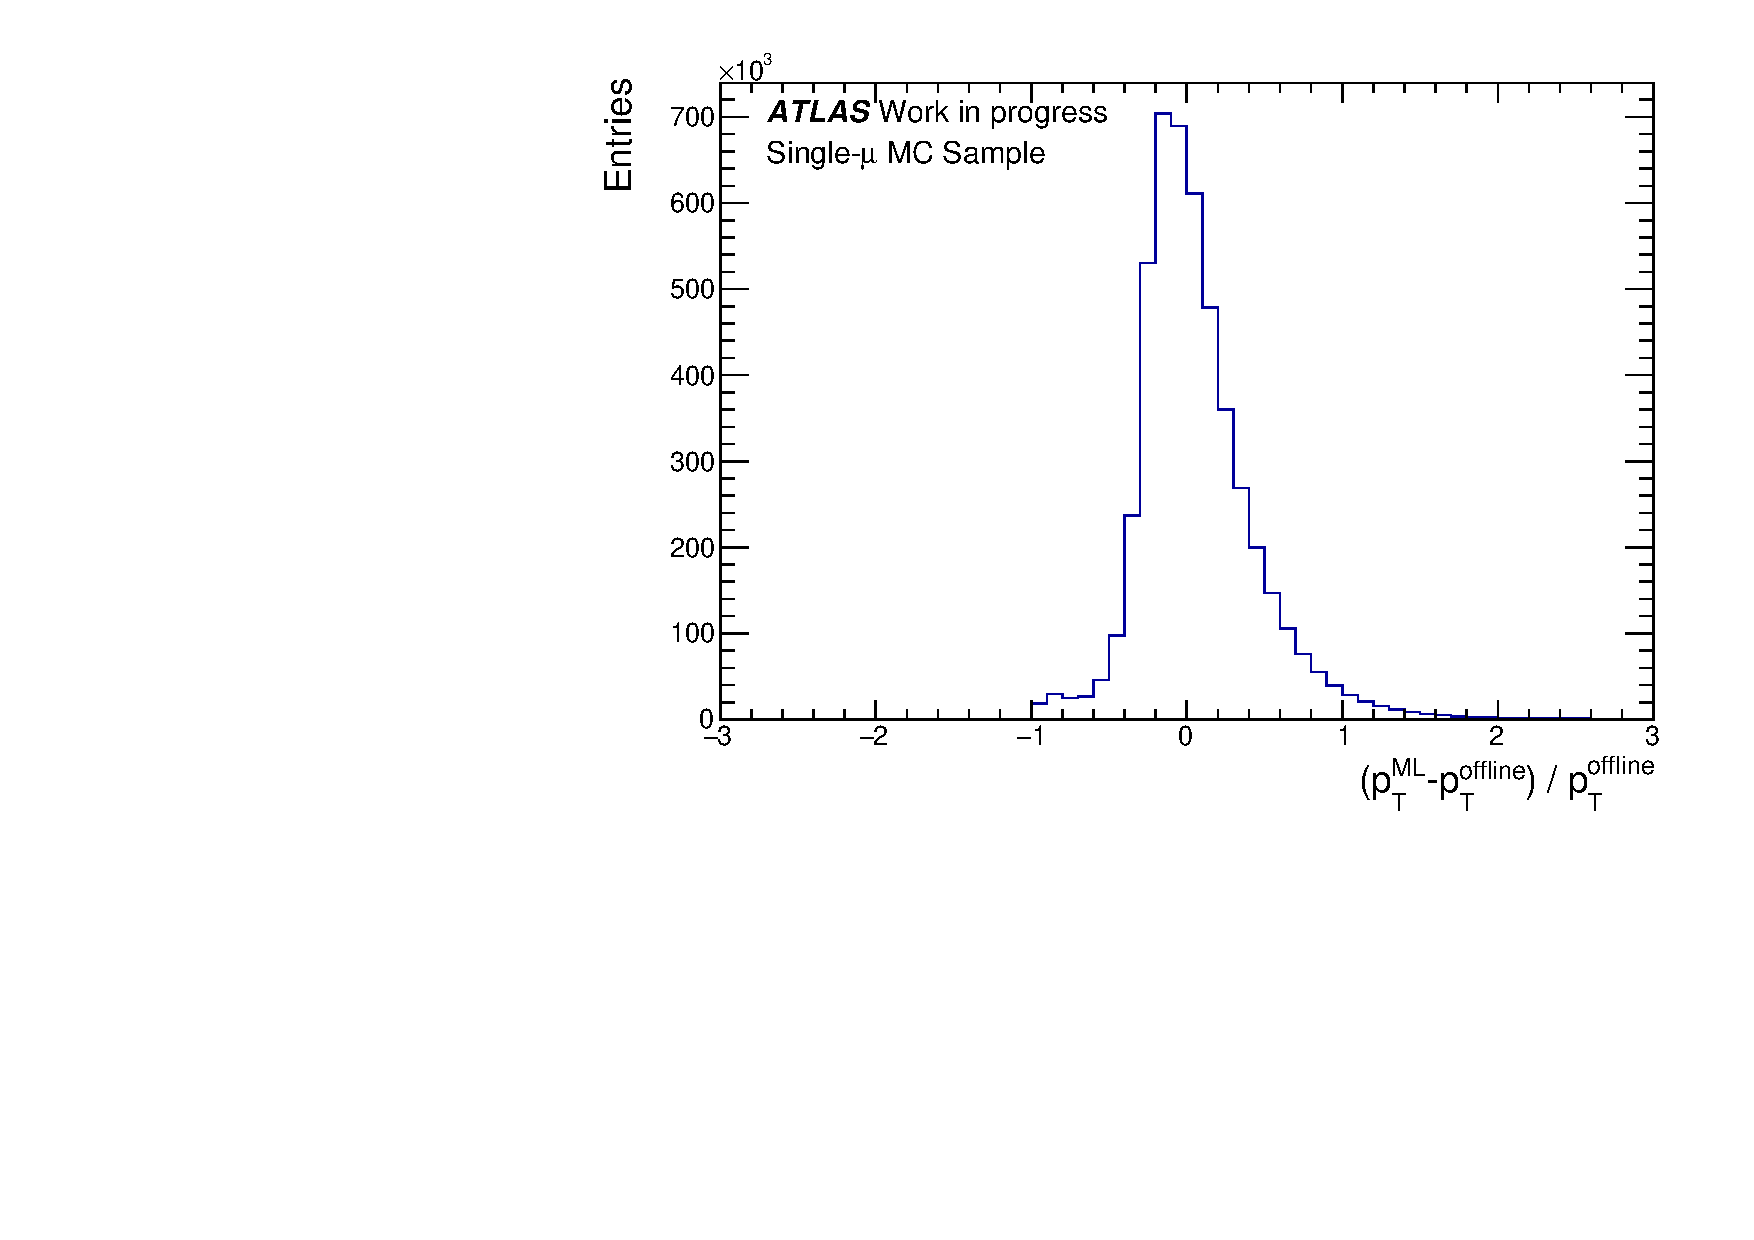
\includegraphics[clip, width=8cm]{fig/4/MC_predtrue.pdf}
        %\vspace{5pt}
        \subcaption{}
        \label{fig:predtrue_MC}
    \end{minipage}%
    %\hfill
    \begin{minipage}[b]{0.7\hsize}%
        \centering
        \hspace*{-0.75cm}
        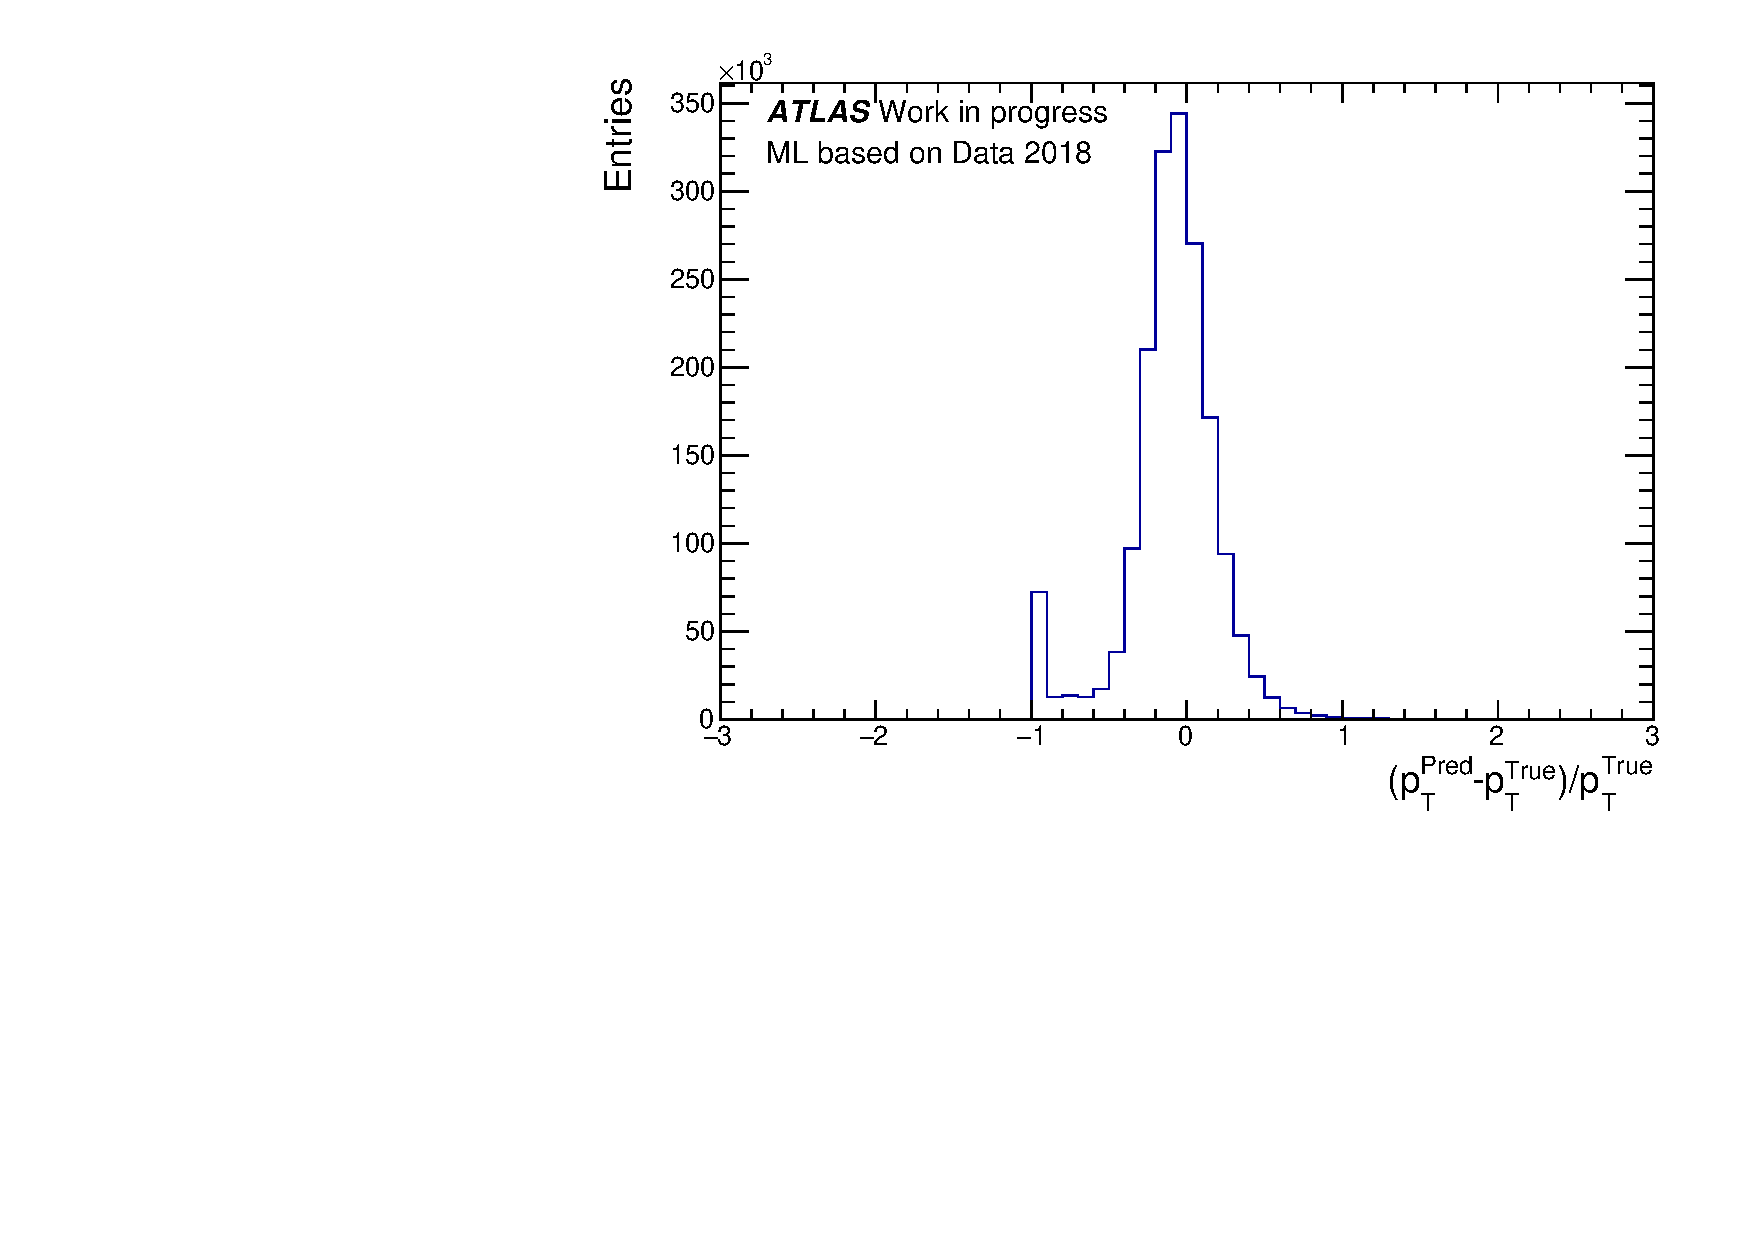
\includegraphics[clip, width=8cm]{fig/4/predtrue.pdf}
        %\vspace{5pt}
        \subcaption{}
        \label{fig:predtrue_Data}
    \end{minipage}%
    \end{tabular}
    \caption{学習に用いた正解値($p_{\rm{T}}^{True}$)と予測値($p_{\rm{T}}^{Pred}$)の残差分布。(b):シミュレーションデータを用いてトレーニングを行ったMLP。(b):2018年Run-2のデータを用いてトレーニングを行ったMLP。}
    \label{fig:predtrue}
\end{figure}

%\begin{figure}[htb]
%  \centering
%  %\rule{8cm}{6cm}
%  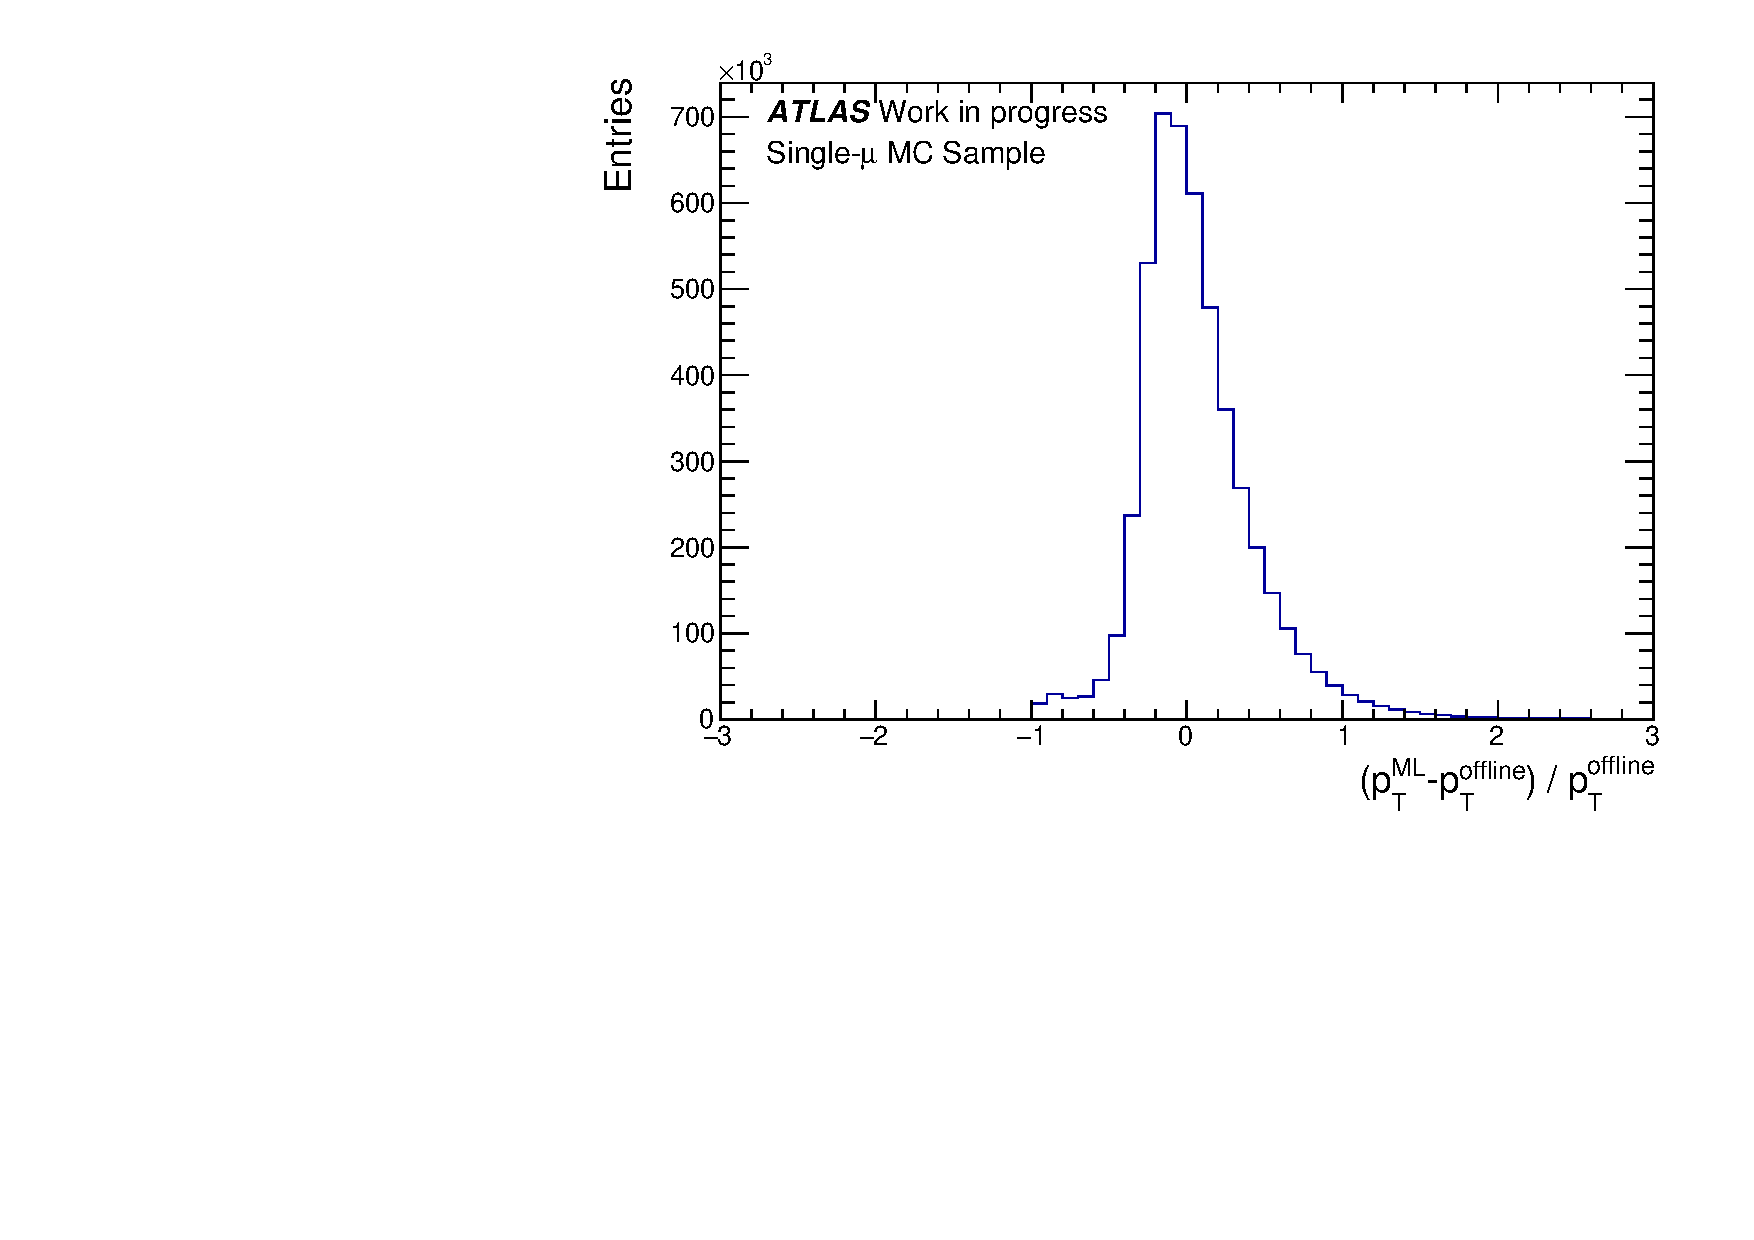
\includegraphics[clip, width=10cm]{fig/4/MC_predtrue.pdf}
%  \caption{学習に用いた正解値($p_{\rm{T}}^{True}$)と予測値($p_{\rm{T}}^{Pred}$)の残差の分布。}
%  \label{fig:MC_predtrue}
%\end{figure}
\begin{figure}
    %\centering
    \begin{tabular}{cc}
    \centering
    \begin{minipage}[b]{0.45\hsize}%
        \centering
        \hspace*{-1.5cm}
        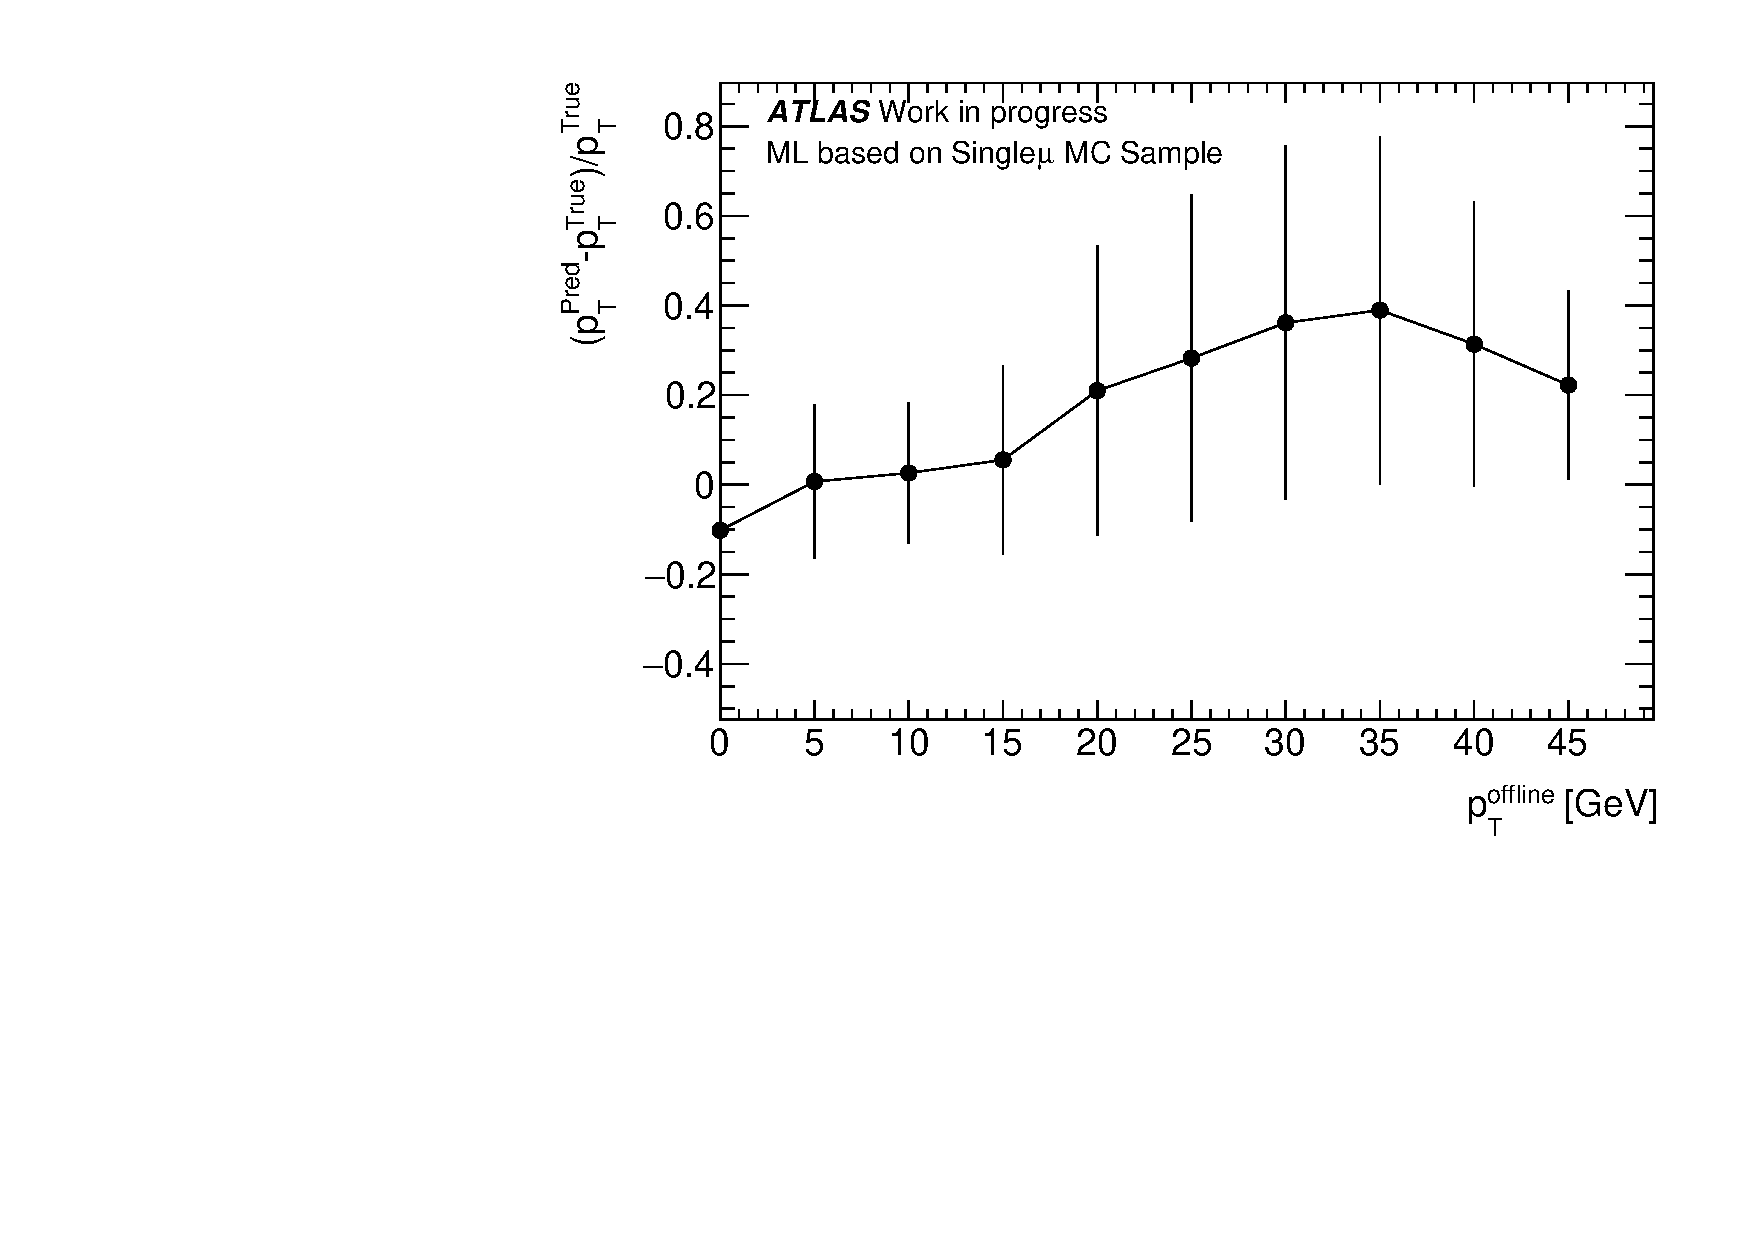
\includegraphics[clip, width=8cm]{fig/4/MC_predtrue_perpt.pdf}
        %\vspace{5pt}
        \subcaption{}
        \label{Gauspredtrue_MC}
    \end{minipage}%
    %\hfill
    \begin{minipage}[b]{0.7\hsize}%
        \centering
        \hspace*{-0.5cm}
        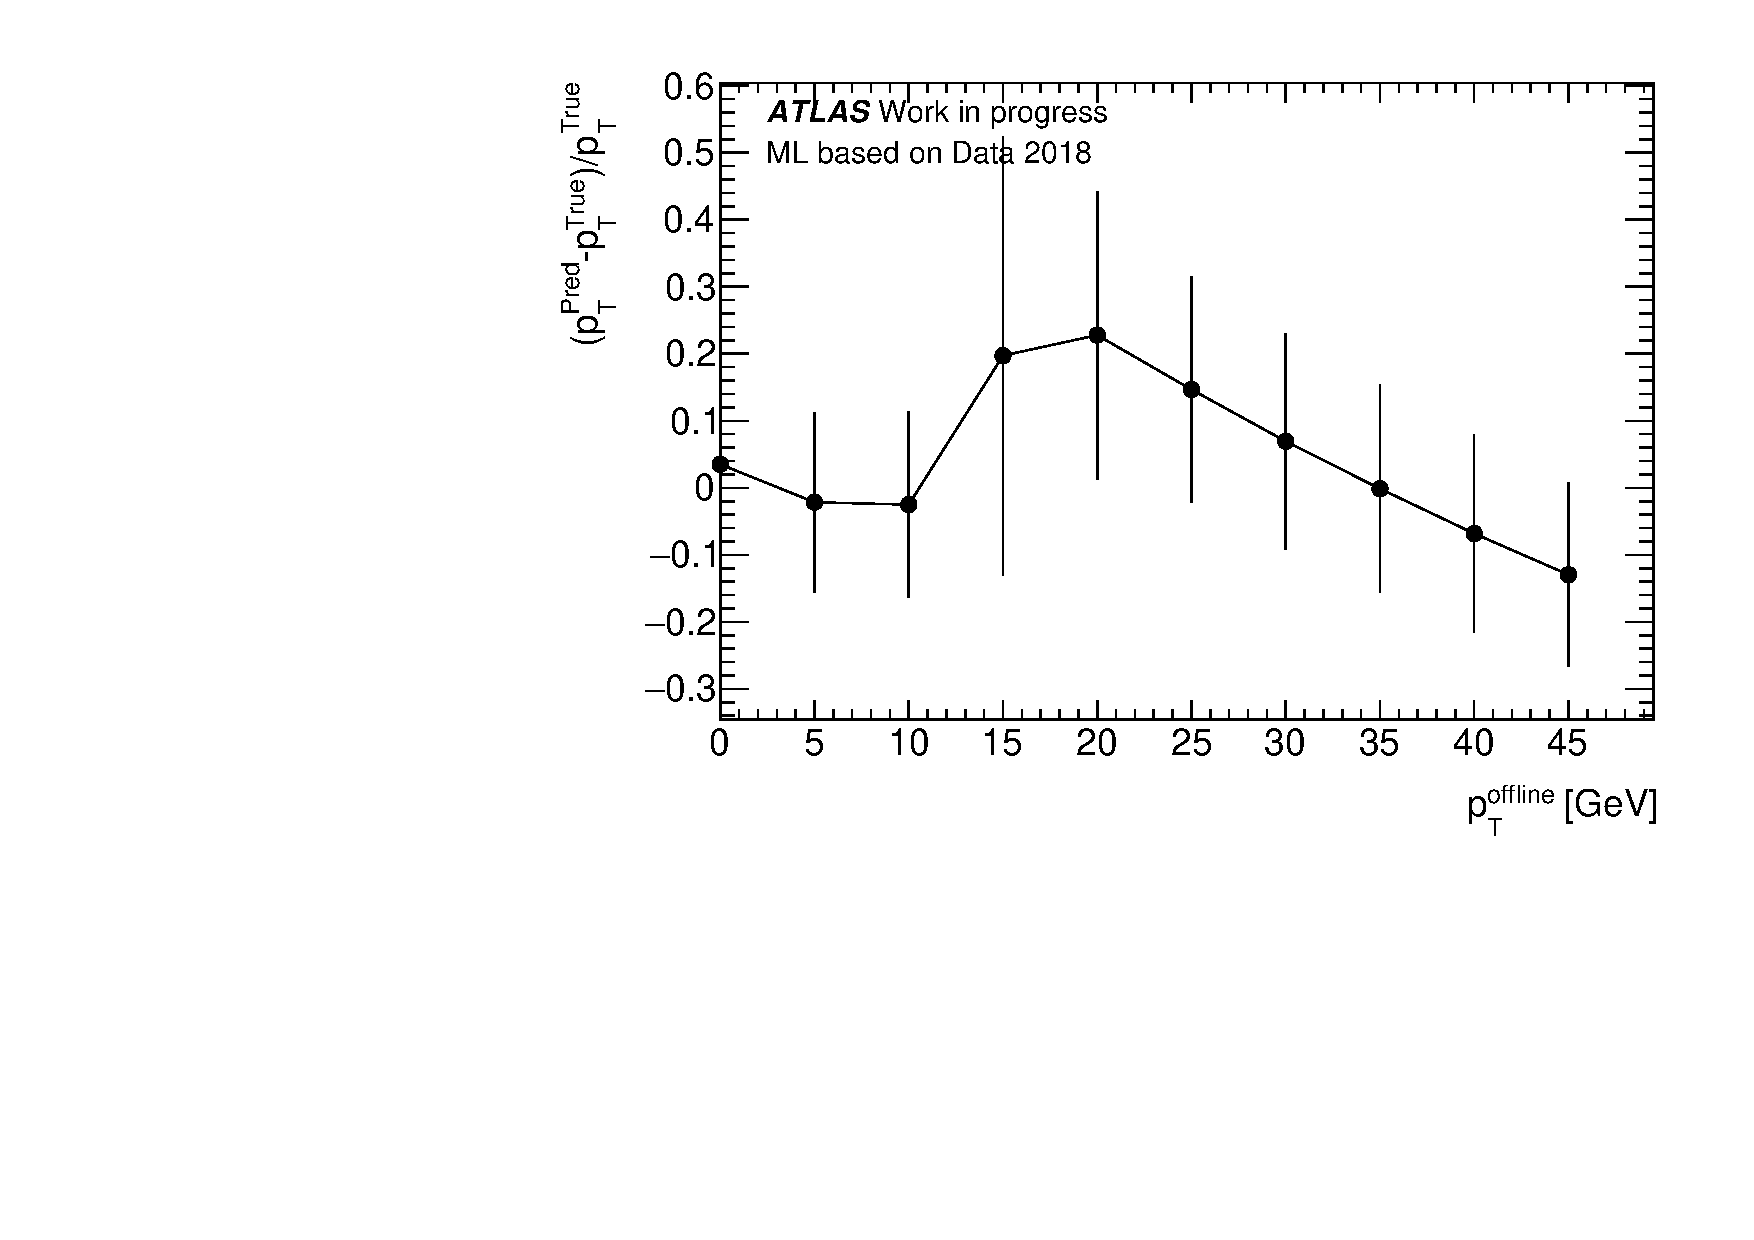
\includegraphics[clip, width=8cm]{fig/4/predtrue_perpt.pdf}
        %\vspace{5pt}
        \subcaption{}
        \label{Gauspredtrue_data}
    \end{minipage}%
    \end{tabular}
    \caption{ある$p_{\rm{T}}^{True}$に対して、$p_{\rm{T}}^{Pred}$の分布をガウシアンフィットした場合のmean値の分布。(b):シミュレーションデータを用いてトレーニングを行ったMLP。(b):2018年Run-2のデータを用いてトレーニングを行ったMLP。}
    \label{Gauspredtrue}
\end{figure}


%\begin{figure}[htb]
%  \centering
  %\rule{8cm}{6cm}
%  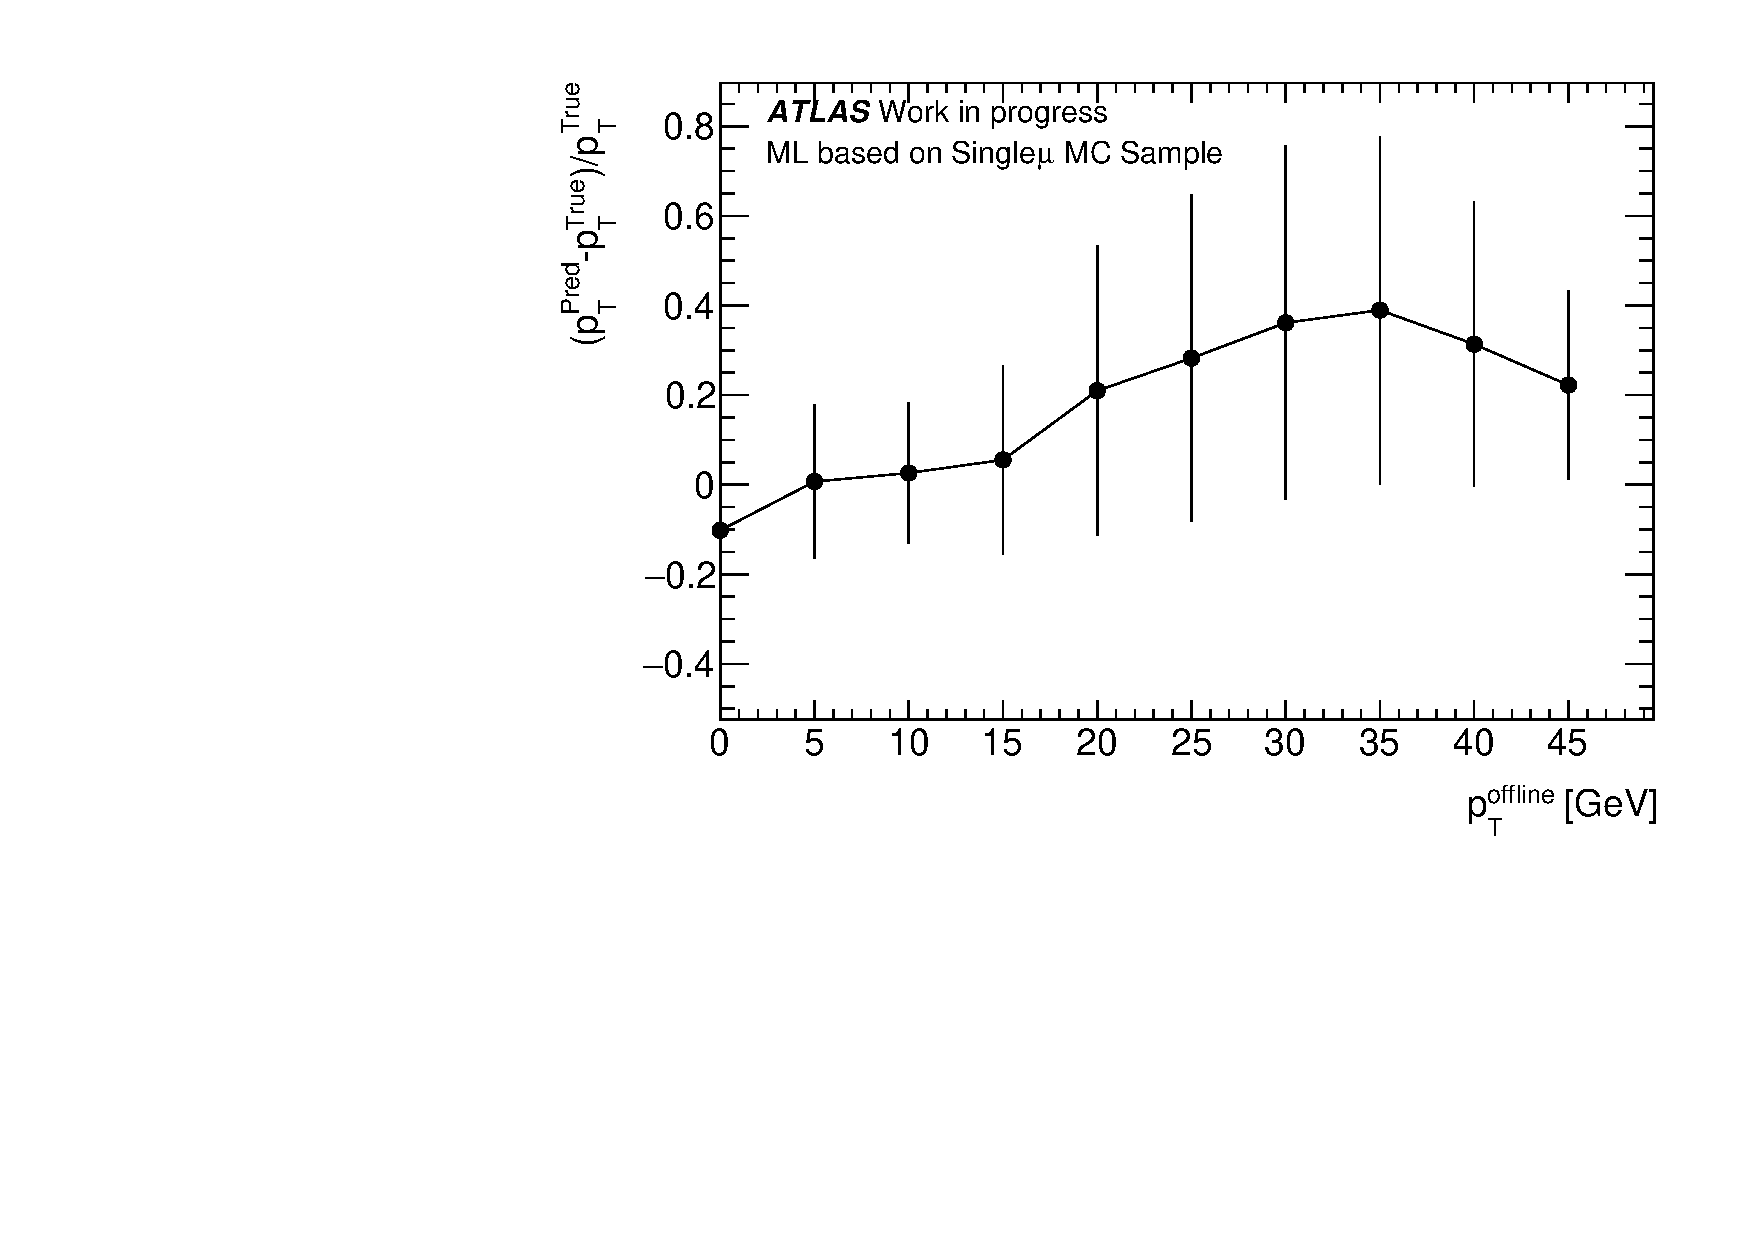
\includegraphics[clip, width=10cm]{fig/4/MC_predtrue_perpt.pdf}
%  \caption{オフライン再構成されたミューオンの$p_{\rm{T}}^{offline}$に対して、$p_{\rm{T}}^{True}$$-$$p_{\rm{T}}^{Pred}$のガウシアンフィットした時のmean値の分布。}
%  \label{fig:MC_predtrue_perpt}
%\end{figure}

%次に、実際のデータをトレーニングに使用した機械学習モデルの評価を行う。
%2018年Run-2で収集したデータを用いて、MLP で予測した$p_{\rm{T}}^{pred}$と正解値 $p_{\rm{T}}^true$の残差分布の比較を行った結果を図~\ref{fig:zannsa_25_Data}に示す。また、ある$p_{\rm{T}}^{True}$に対して、$p_{\rm{T}}^{Pred}$の分布をガウシアンフィットした場合の$\mu$の分布を図~\ref{fig:Gausmu_Data}に示す。こちらも$p_{\rm{T}}^{True}$に対して機械学習の予測値はほぼ線形である事が見て取れる。

%\begin{figure}[htb]
%  \centering
%  %\rule{8cm}{6cm}
%  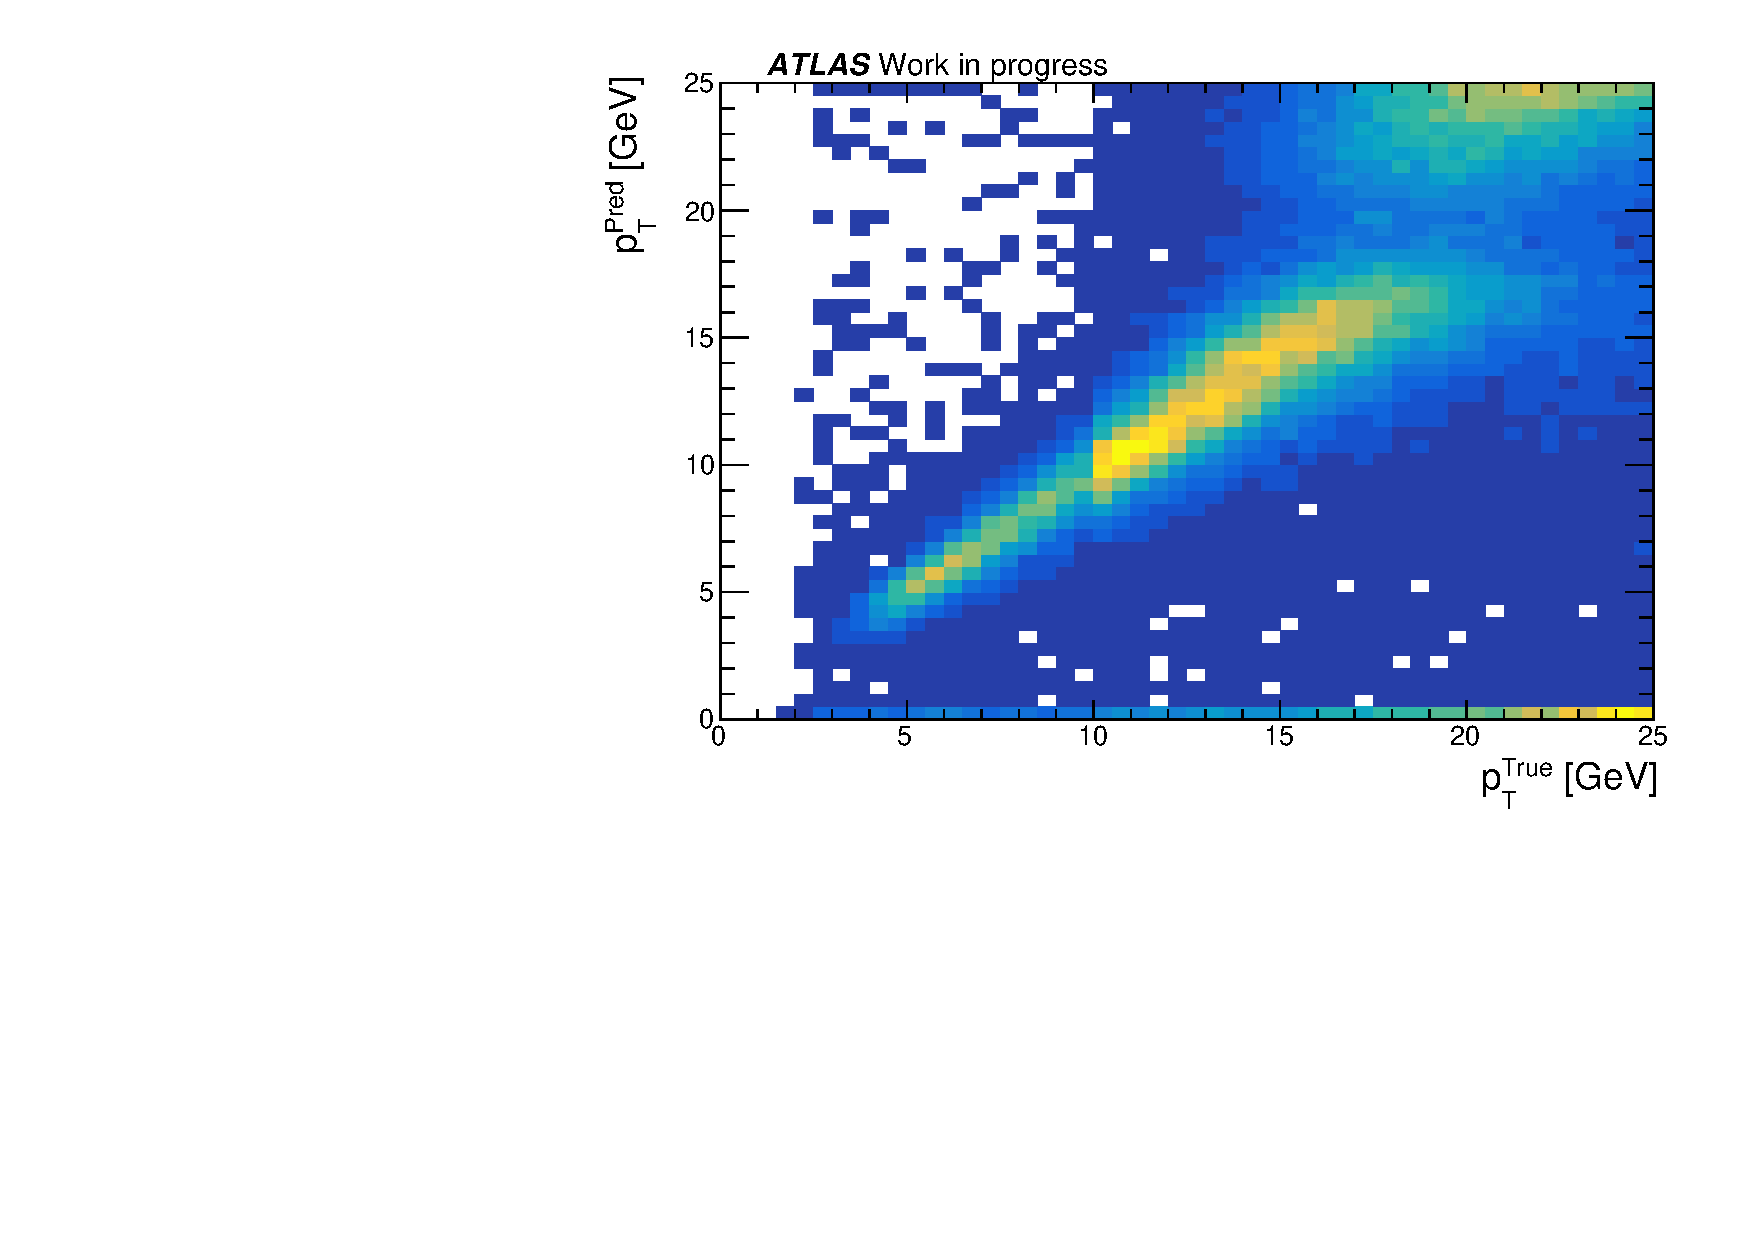
\includegraphics[clip, width=10cm]{fig/4/pred_true_25.pdf}
%  \caption{2018年Run-2のデータを用いてトレーニングを行ったMLPの$p_{\rm{T}}^{True}$に対する$p_{\rm{T}}^{Pred}$の分布。評価には2018年Run-2のデータを用いた。}
%  \label{fig:zannsa_25_Data}
%\end{figure}

%\begin{figure}[htb]
%  \centering
  %\rule{8cm}{6cm}
%  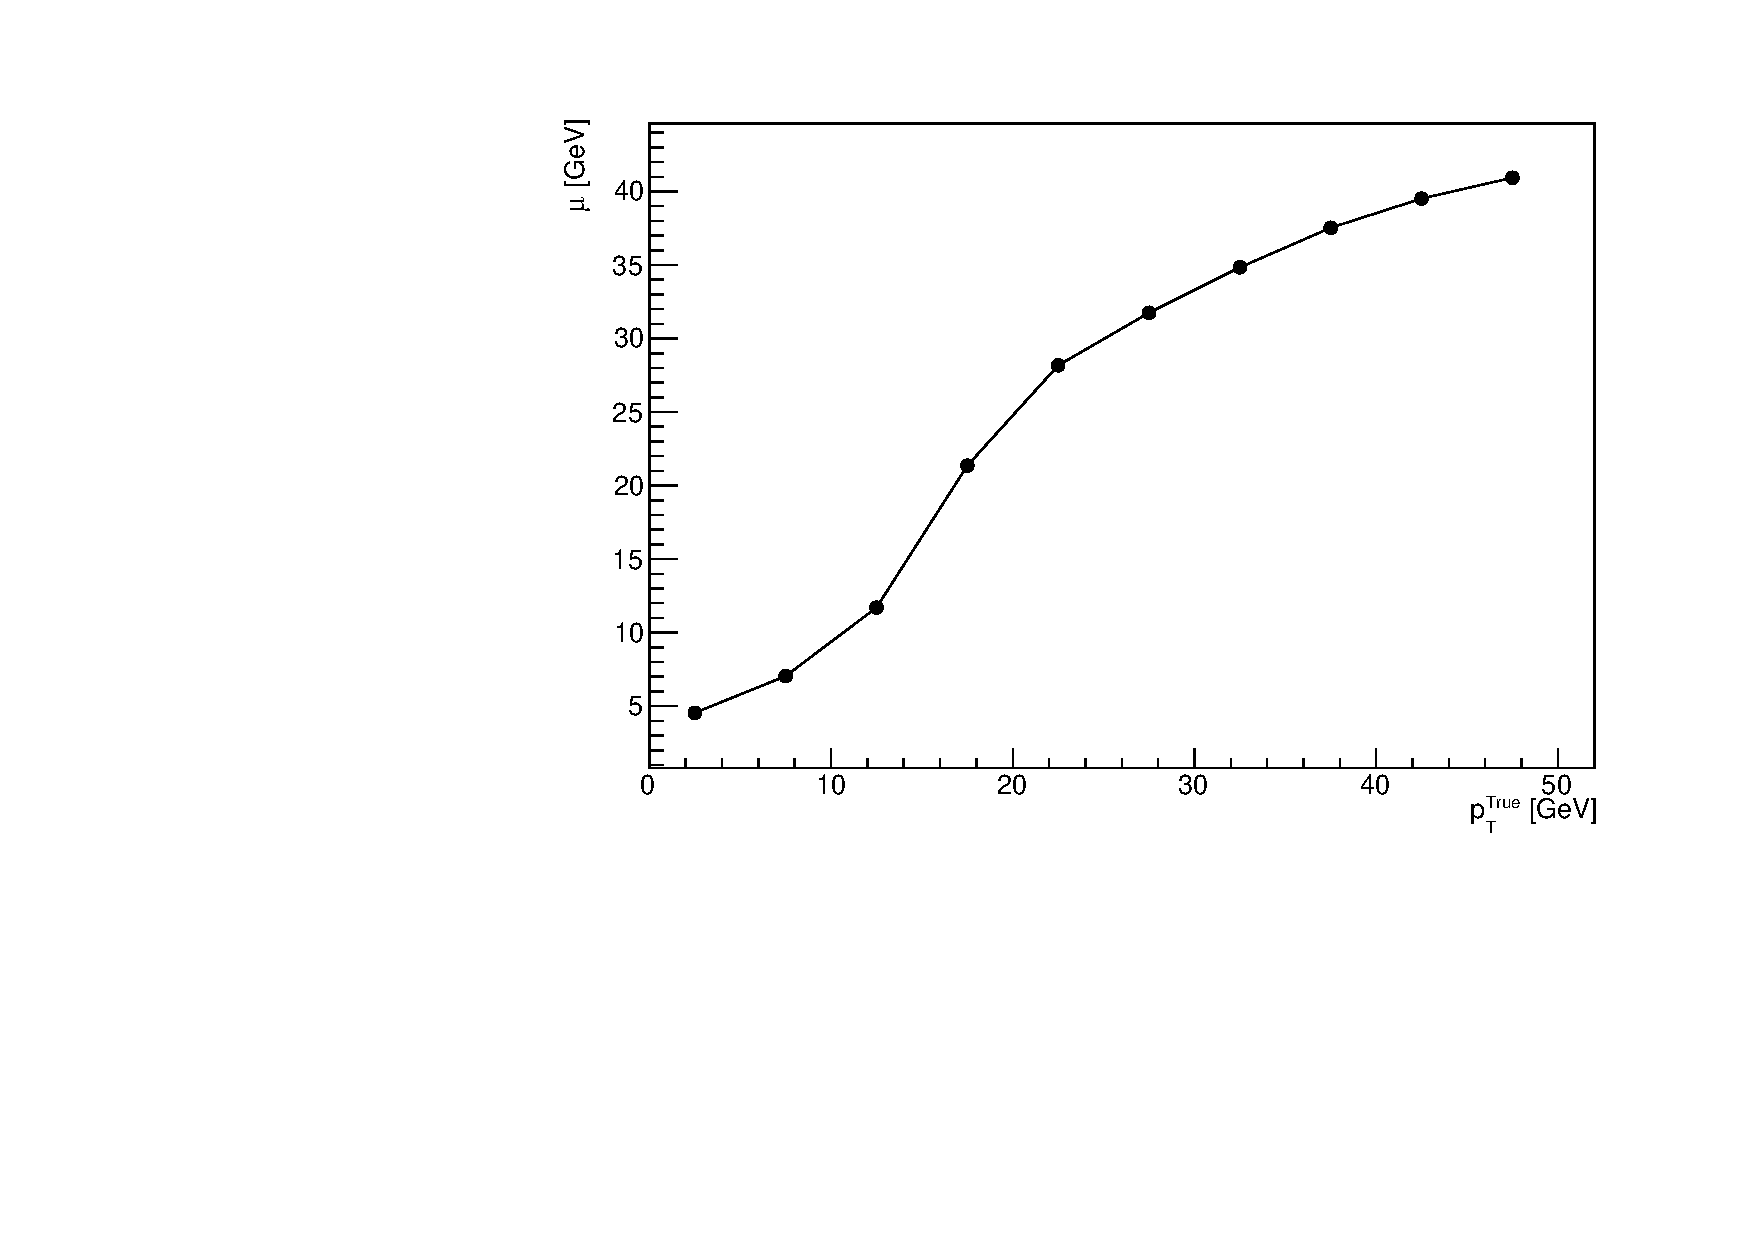
\includegraphics[clip, width=10cm]{fig/4/tp_Gausmean_Data.pdf}
%  \caption{ある$p_{\rm{T}}^{True}$に対して、$p_{\rm{T}}^{Pred}$の分布をガウシアンフィットした時ののmean値の分布。}
%  \label{fig:Gausmu_Data}
%\end{figure}

%\begin{figure}[htb]
% \centering
  %\rule{8cm}{6cm}
%  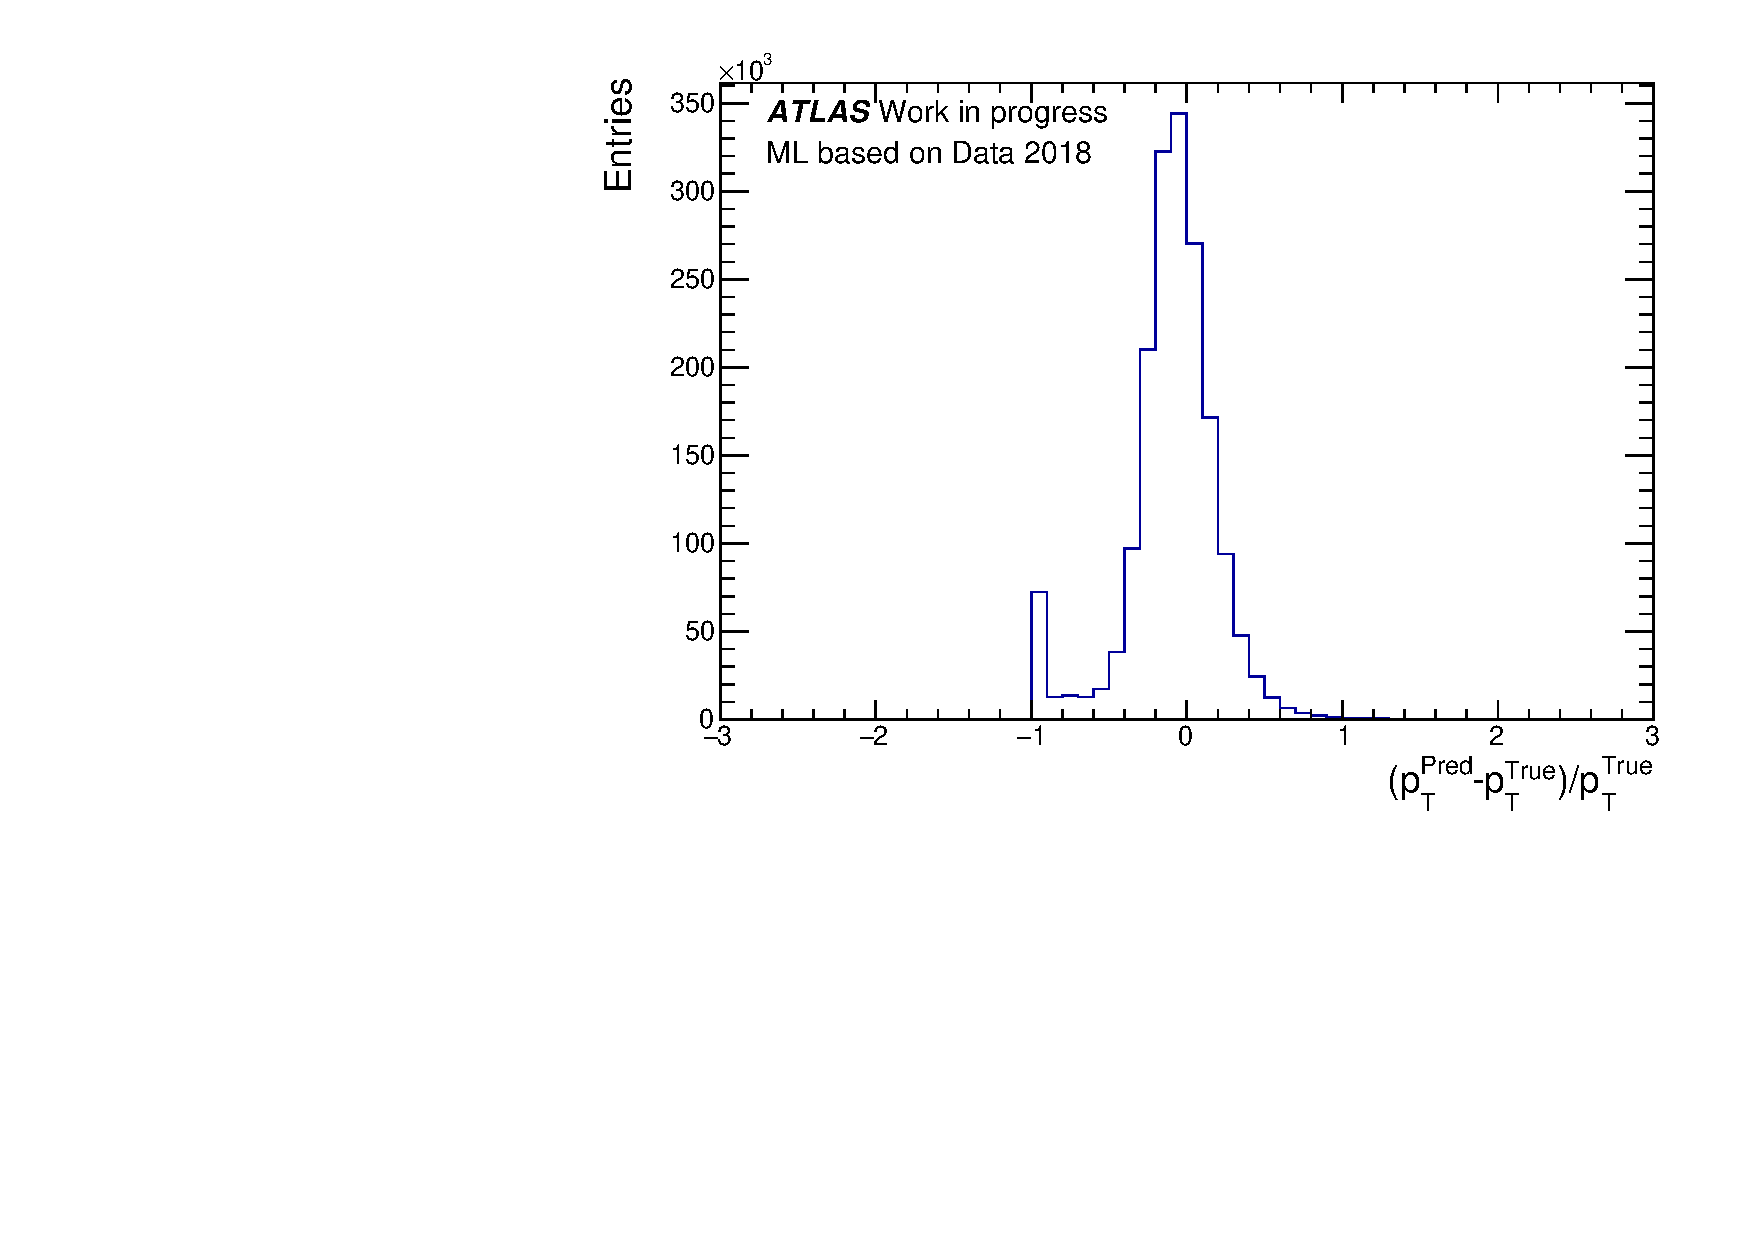
\includegraphics[clip, width=10cm]{fig/4/predtrue.pdf}
%  \caption{学習に用いた正解値($p_{\rm{T}}^{True}$)と予測値($p_{\rm{T}}^{Pred}$)の残差の分布。}
%  \label{fig:Gausmu_Data}
%\end{figure}

%\begin{figure}[htb]
%  \centering
  %\rule{8cm}{6cm}
%  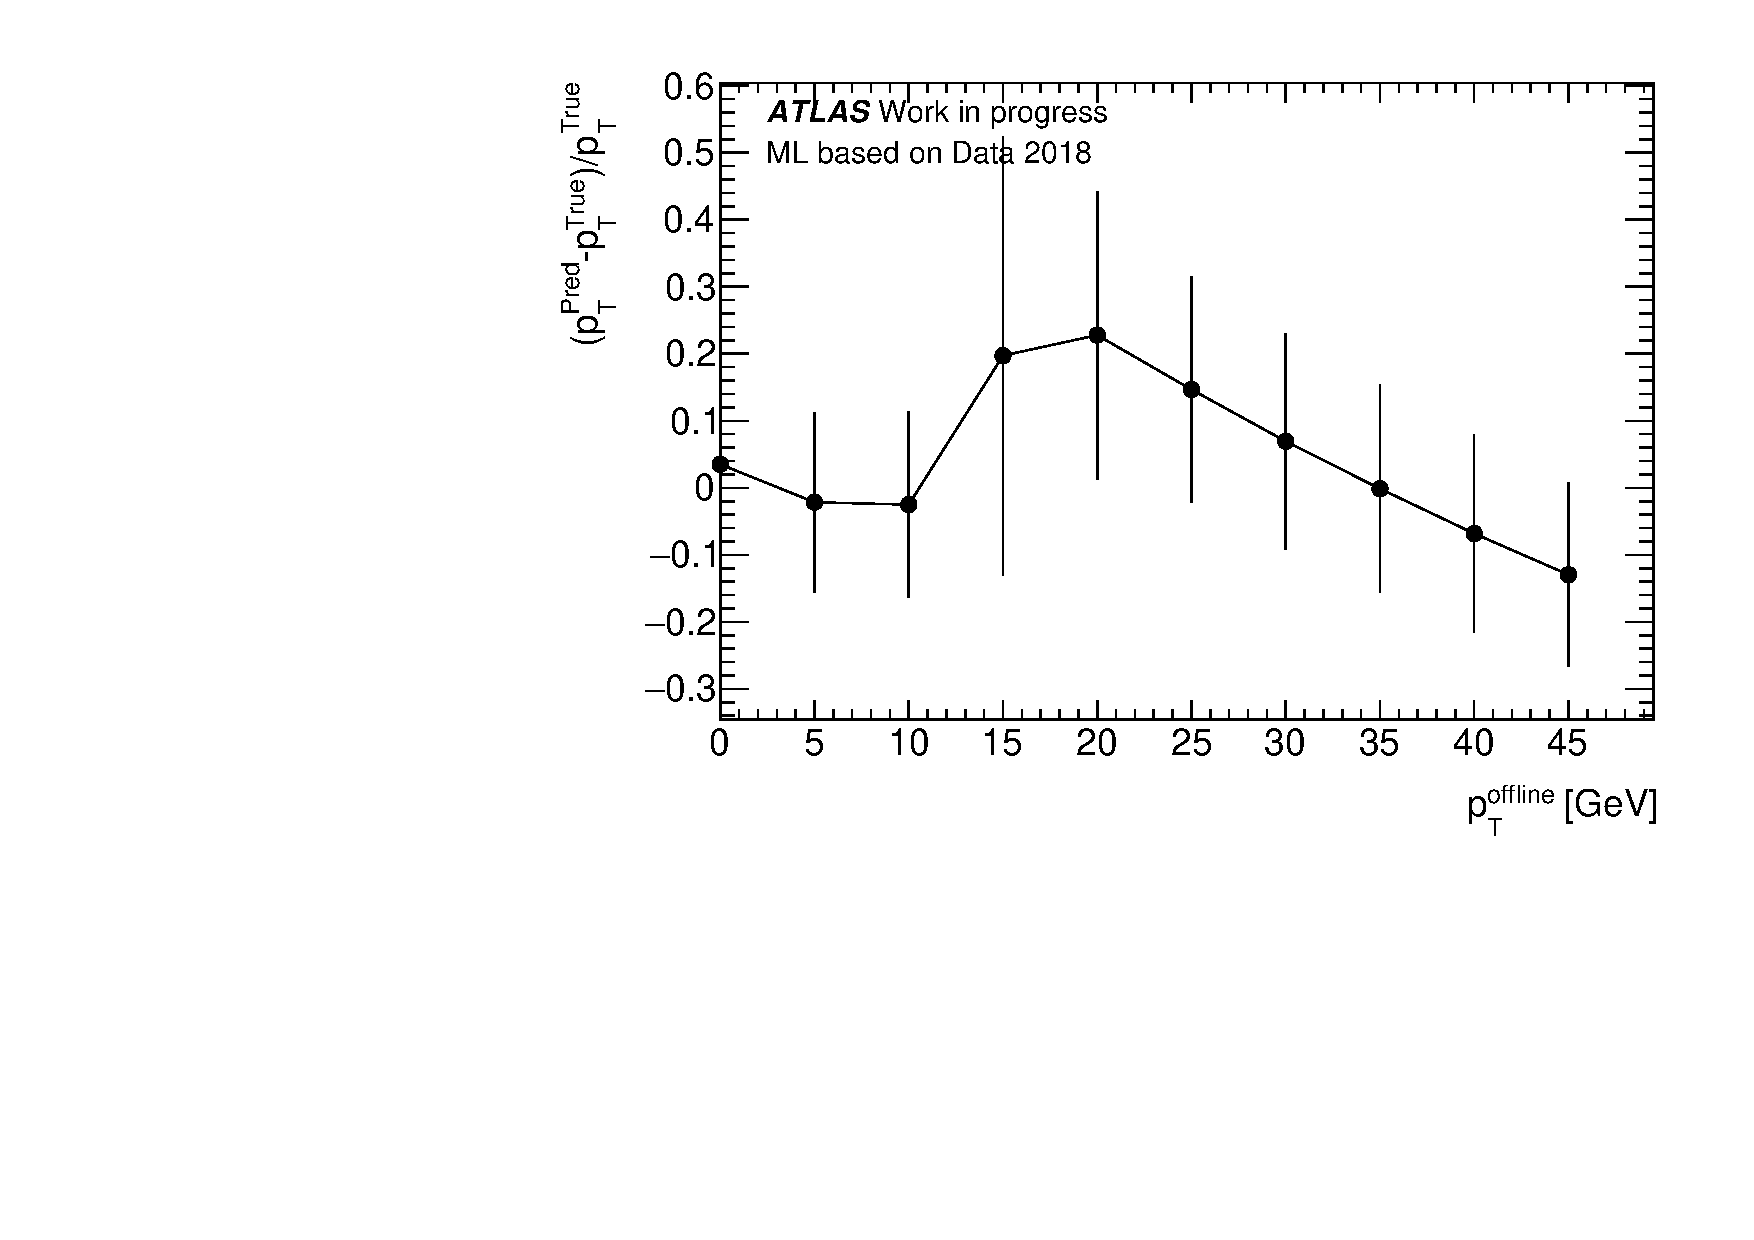
\includegraphics[clip, width=10cm]{fig/4/predtrue_perpt.pdf}
%  \caption{オフライン再構成されたミューオンの$p_{\rm{T}}^{offline}$に対して、$p_{\rm{T}}^{True}$$-$$p_{\rm{T}}^{Pred}$のガウシアンフィットした時のmean値の分布。}
%  \label{fig:Gausmu_Data}
%\end{figure}

\newpage
\subsection{出力データをPt閾値に変換}
\subsubsection{トリガー効率の算出}
全オフライン再構成されたミューオンの内、あるpT 閾値以上のトリガーが発行された割合$\epsilon$を式~\eqref{equ:Eff}と定義し、トリガー効率の算出を行った。
このとき得られるトリガー効率を $p_{\rm{T}}$の関数で表したプロットをTurn-on curveと呼ぶ。
\begin{equation}
    \epsilon = \frac{ある p_{\rm{T}} 閾値以上のトリガーを発行したミューオンの数}{全オフライン再構成したミューオンの数}
 \label{equ:Eff}
\end{equation}


\subsubsection{フィッティング関数の定義}\label{section:fitting}
式~\eqref{equ:fitting}を用いて Turn-on curve にフィッティングを行うことでトリガー効率を定量的に評価する。
\begin{equation}
    f(p_{\rm{T}}) = \frac{p_0}{exp(\frac{p_{\rm{T}}-p_1}{p_2})+1}
 \label{equ:fitting}
\end{equation}
ここで、トリガーの性能を表す 3 つのパラメータ $p_0$, $p_1$, $p_2$を以下のように定義する。Turn-on curveにフィッティングした様子を図~\ref{fig:fiting}に示す。
\begin{figure}[tb]
  \centering
  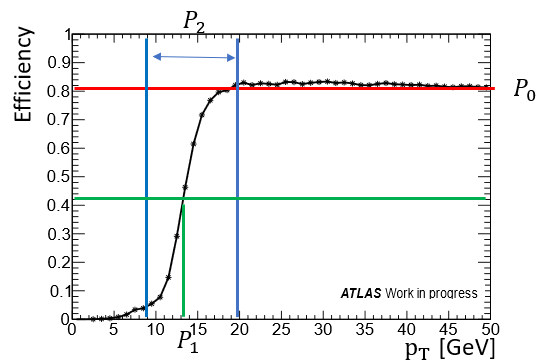
\includegraphics[clip, width=12cm]{fig/4/fitting_def.png}
  \caption{Turn-on curve に対するfittingの例。$p_0$を Plateau efficiency、$p_1$を Effective threshold、$p_2$を Resolution と定義する。}
  \label{fig:fiting}
\end{figure}

\begin{enumerate}\label{table:fitting}
   \item $p_0$:Plateau efficiency\\
   Turn-on curve が横這いになった時のトリガー効率を表す。トリガー閾値以上の pT を持つミューオンに対するトリガー効率を表すため、その値が 1 に近い方が高性能である。
   \item $p_1$:Effective threshold\\
   トリガーの実効的な $p_{\rm{T}}$の閾値を表す。トリガー効率が Plateau efficiency の値の 50\% となる時の $p_{\rm{T}}$の値である。
   \item $p_2$:Resolution\\
   トリガーの運動量の分解能を表す。Turn-on curve の立ち上がりの鋭さに対応すしており、Resolution の値が大きくなると Turn-on curve の立ち上がりが緩くなるため、fトリガーの運動量分解能が悪くなる。
\end{enumerate}

\newpage
\subsubsection{15段階閾値への変換}
図~\ref{fig:all_output}に示すように、目的とする$p_{\rm{T}}$の値はMLPから連続値として出力される。そのため、任意の値で$p_{\rm{T}}$を区切り15段階の$p_{\rm{T}}$閾値に変換を行う。
方法としては、図~\ref{ninninoCut}のように任意の値で$p_{\rm{T}}$を区切った時のトリガー効率を求め、Turn-on curveに対し式\eqref{equ:fitting}を用いてフィッティングを行う。フィッティング結果からEffective thresholdを求め、Effective thresholdが\ref{section:CW}節で述べたRun-3における15段階閾値となる任意の値を導出する。
\begin{figure}[tb]
  \centering
  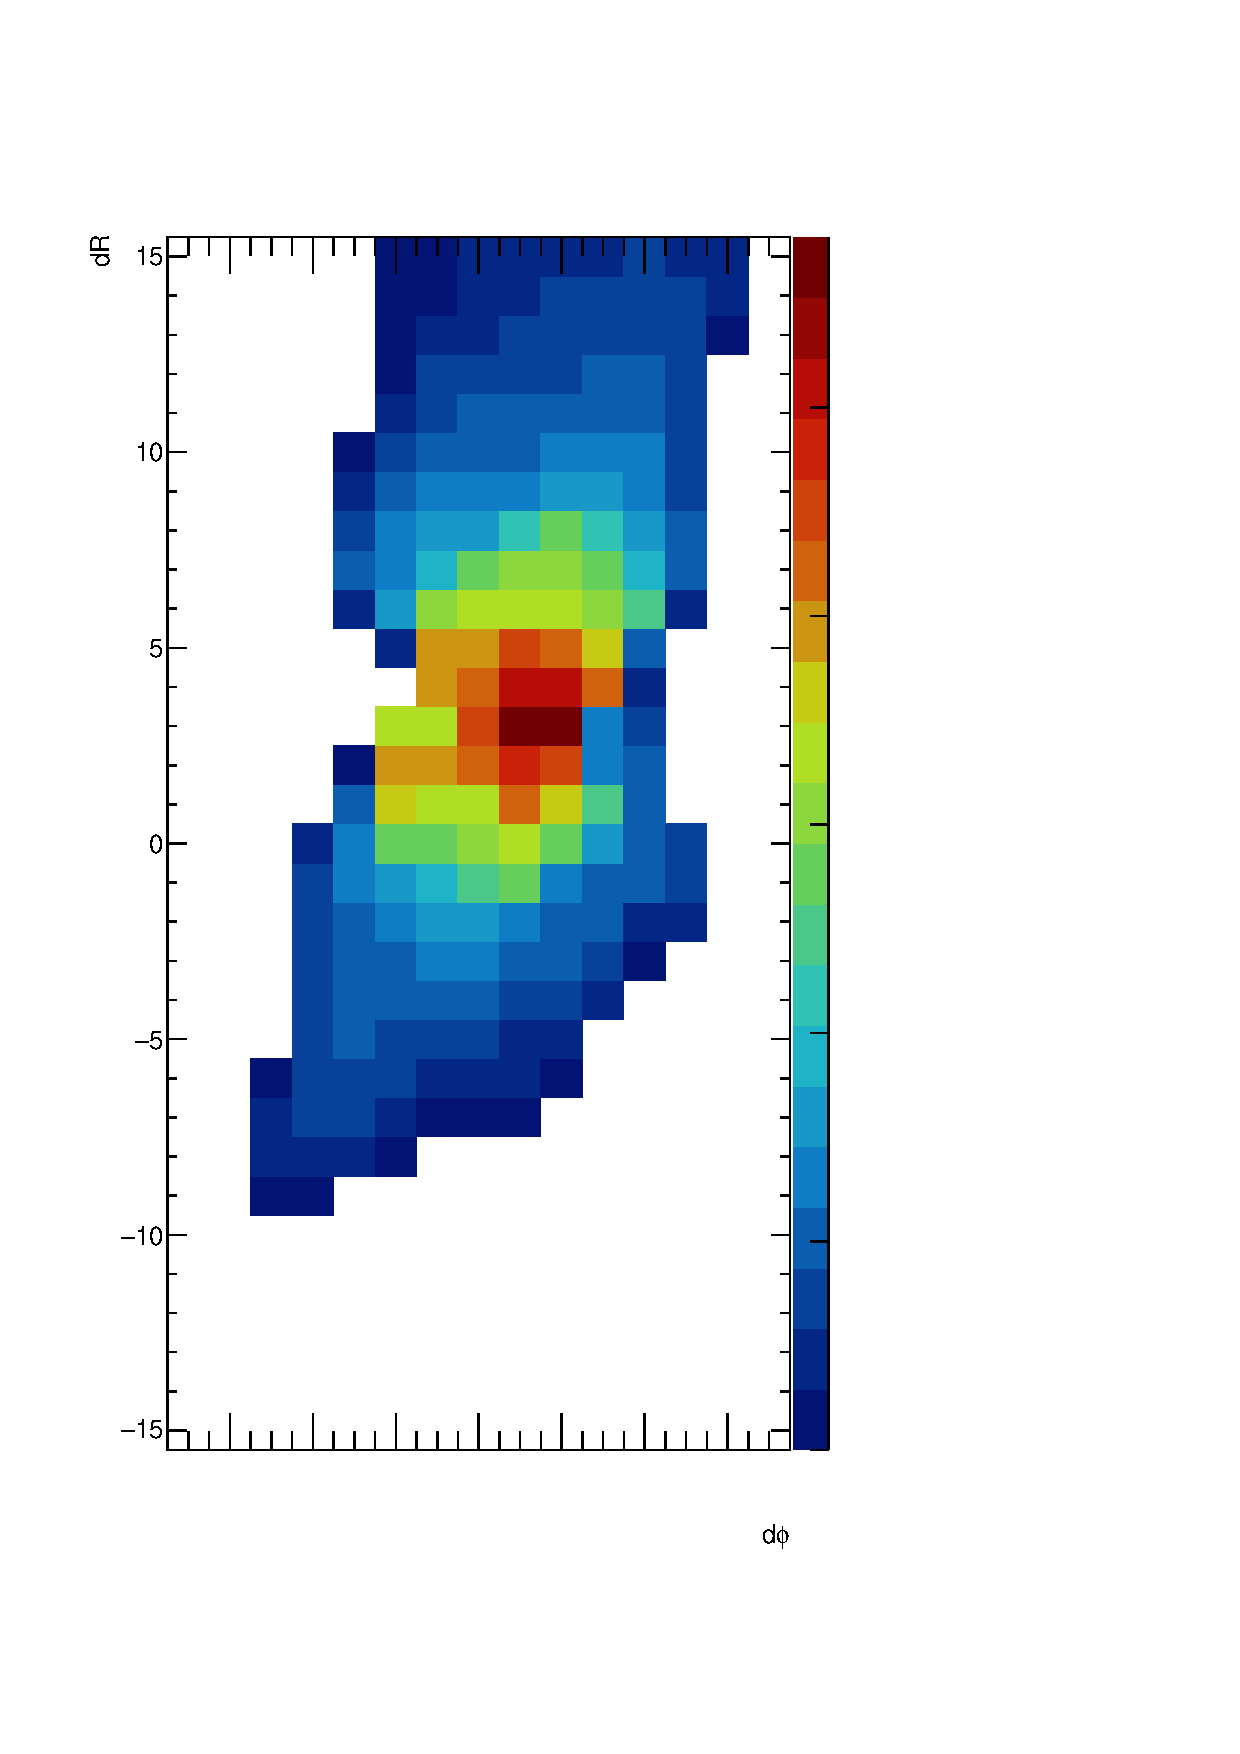
\includegraphics[clip, width=4cm]{fig/4/all_output_rainbow.pdf}
  \caption{MLPから出力された$p_{\rm{T}}$のdR$-$d$phi$分布}
  \label{fig:all_output}
\end{figure}

\begin{figure}
    %\centering
    \begin{tabular}{ccc}
    \centering
    \begin{minipage}[b]{0.33\hsize}%
        \centering
        %\hspace*{-2cm}
        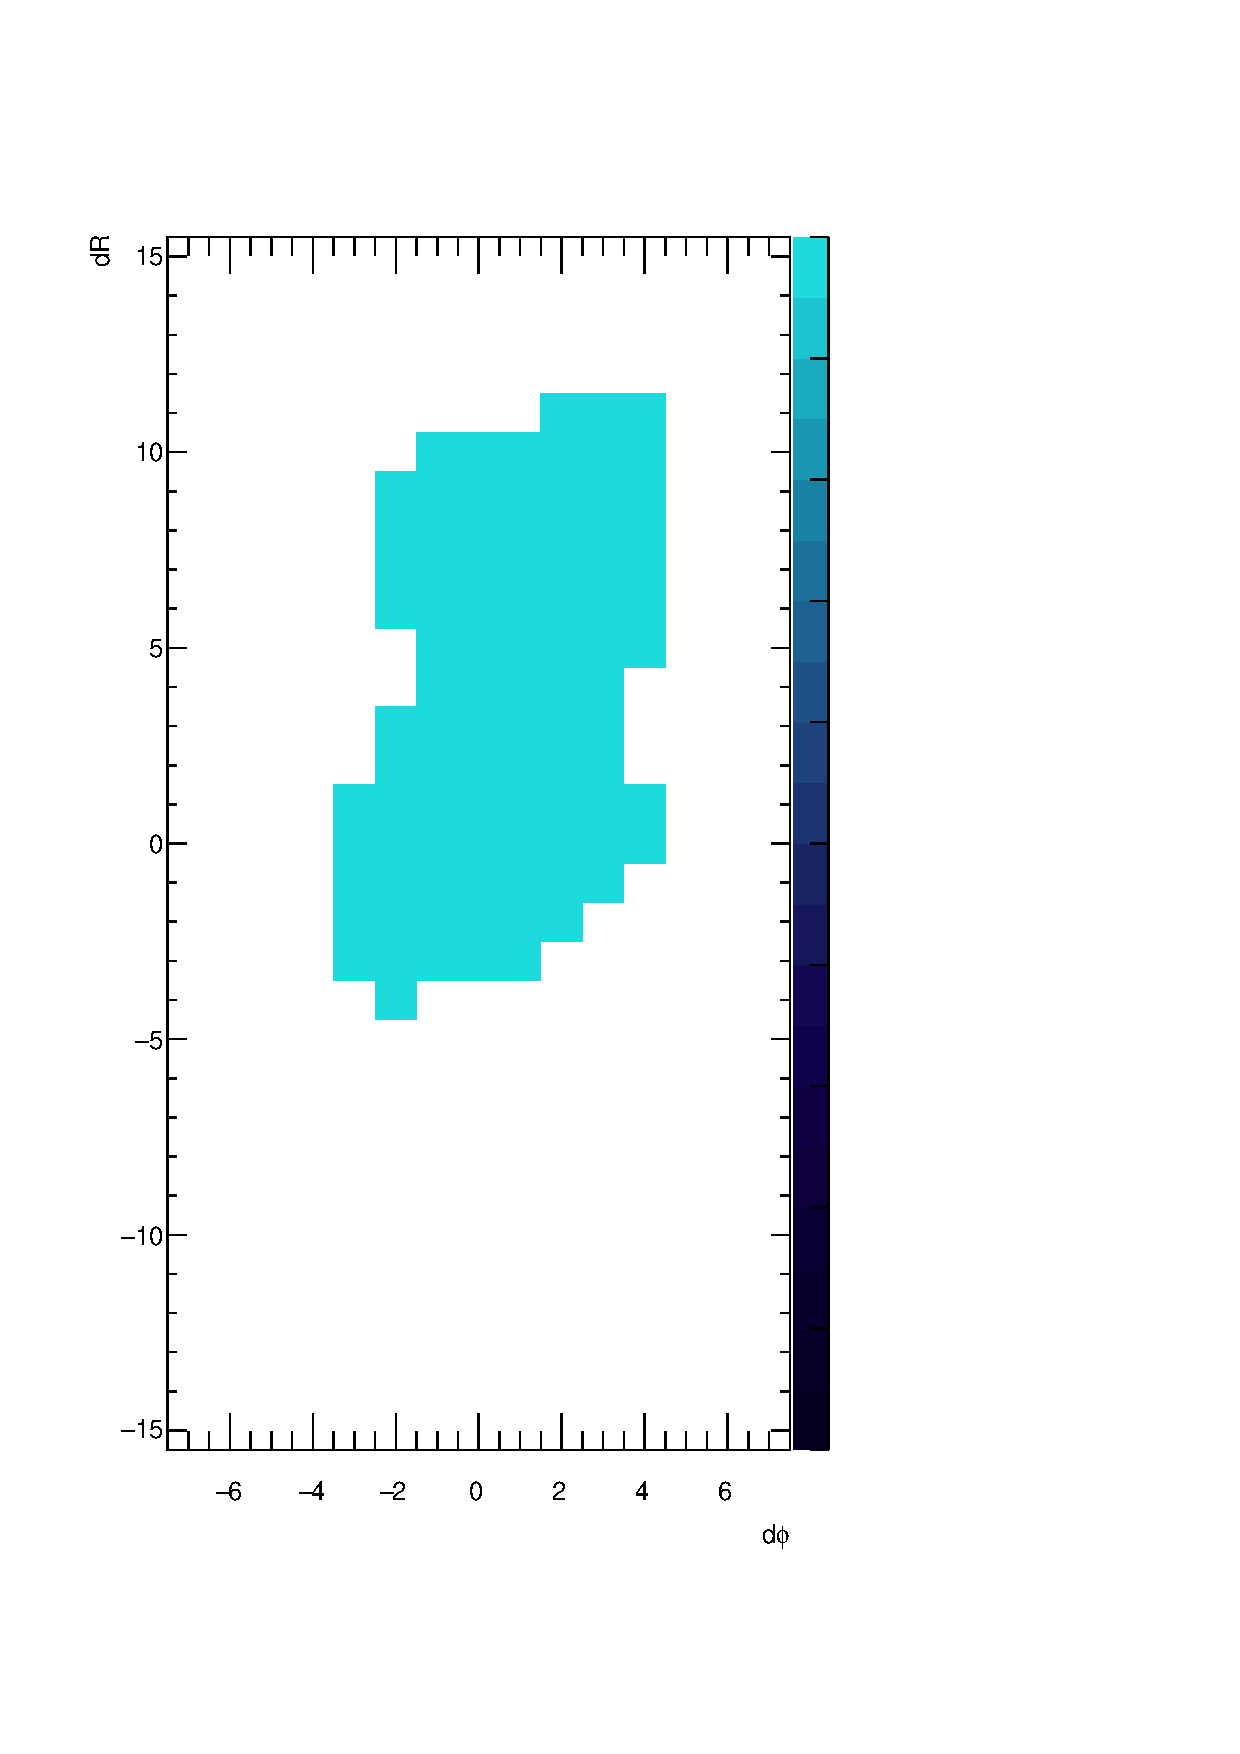
\includegraphics[clip, width=4cm]{fig/4/cut1_output.pdf}
        %\vspace{5pt}
        \subcaption{}
        \label{cut1}
    \end{minipage}%
    %\hfill
    \begin{minipage}[b]{0.33\hsize}%
        \centering
        %\hspace*{-1cm}
        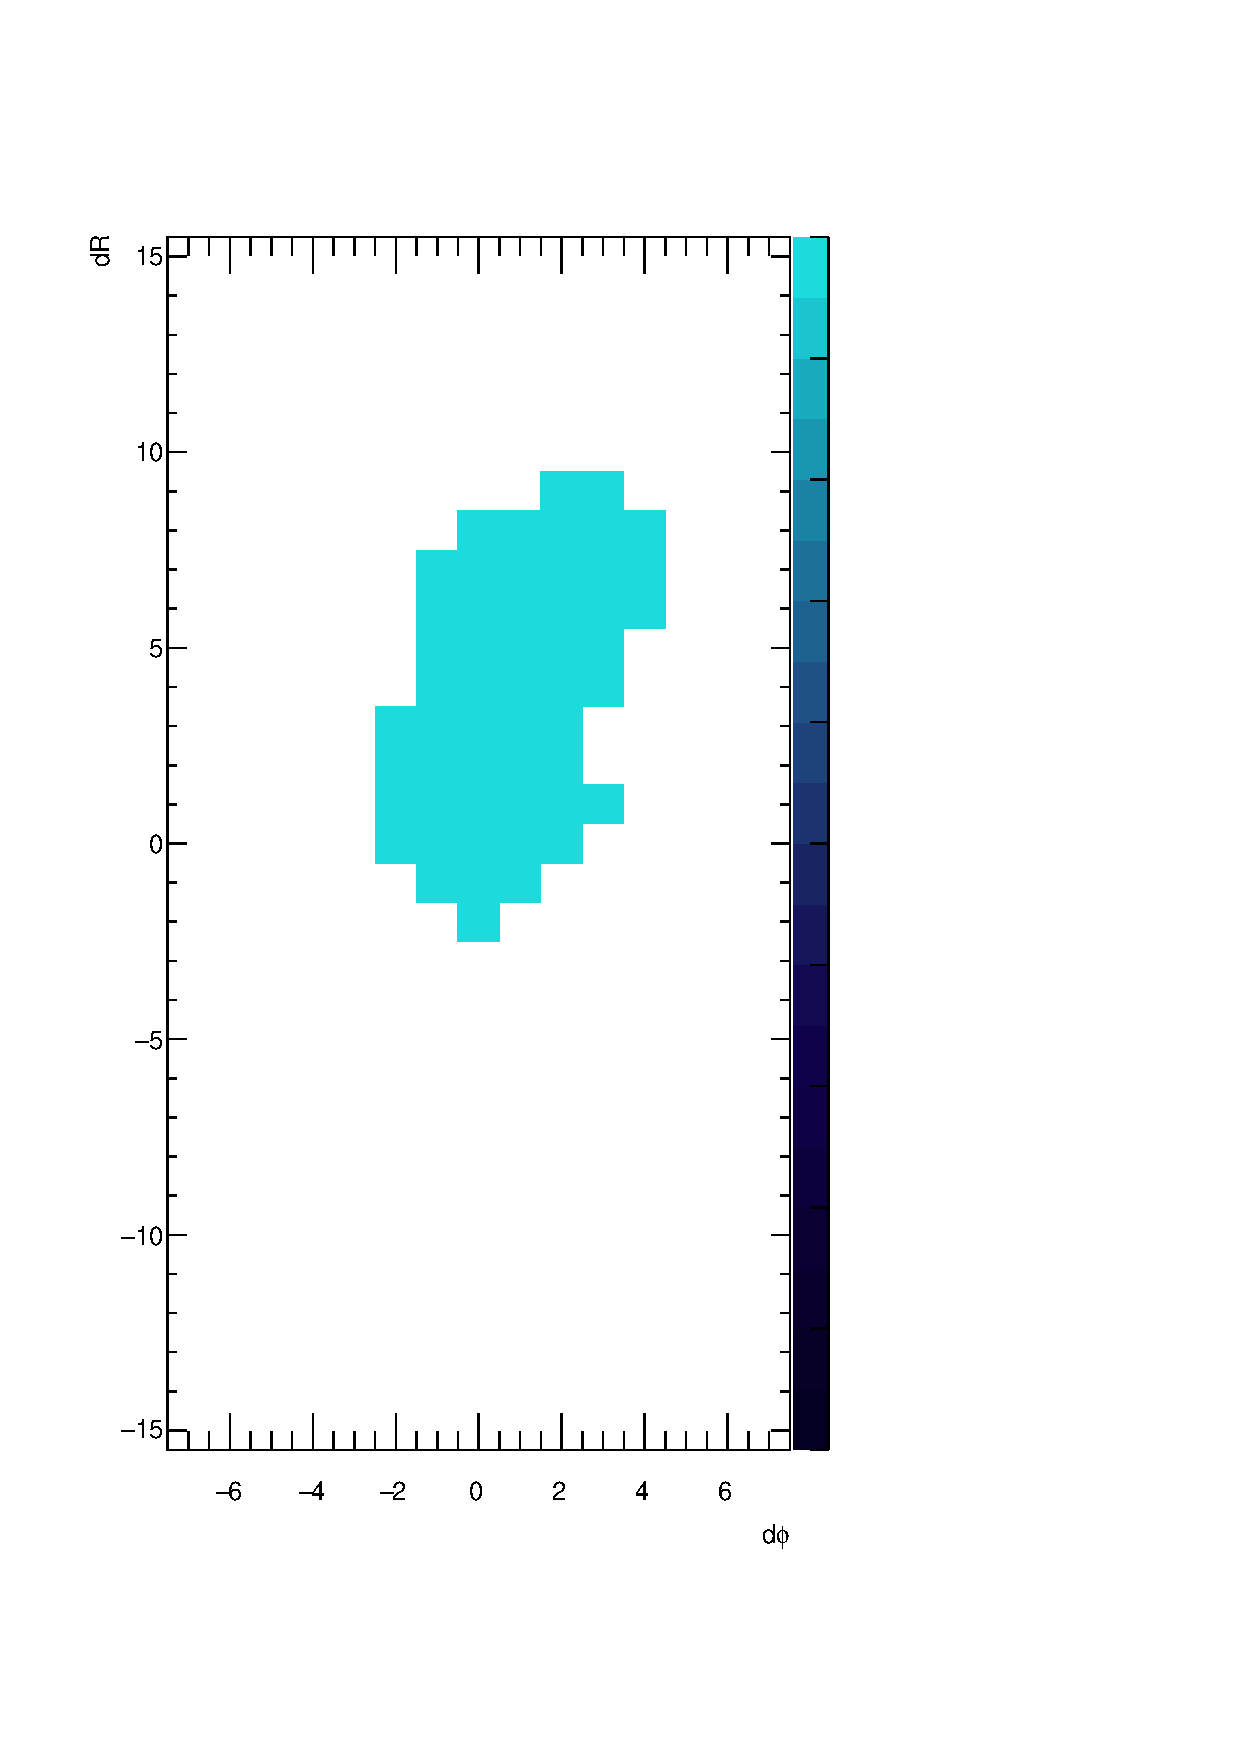
\includegraphics[clip, width=4cm]{fig/4/cut2_output.pdf}
        %\vspace{5pt}
        \subcaption{}
        \label{cut2}
    \end{minipage}%
    \begin{minipage}[b]{0.33\hsize}%
        \centering
        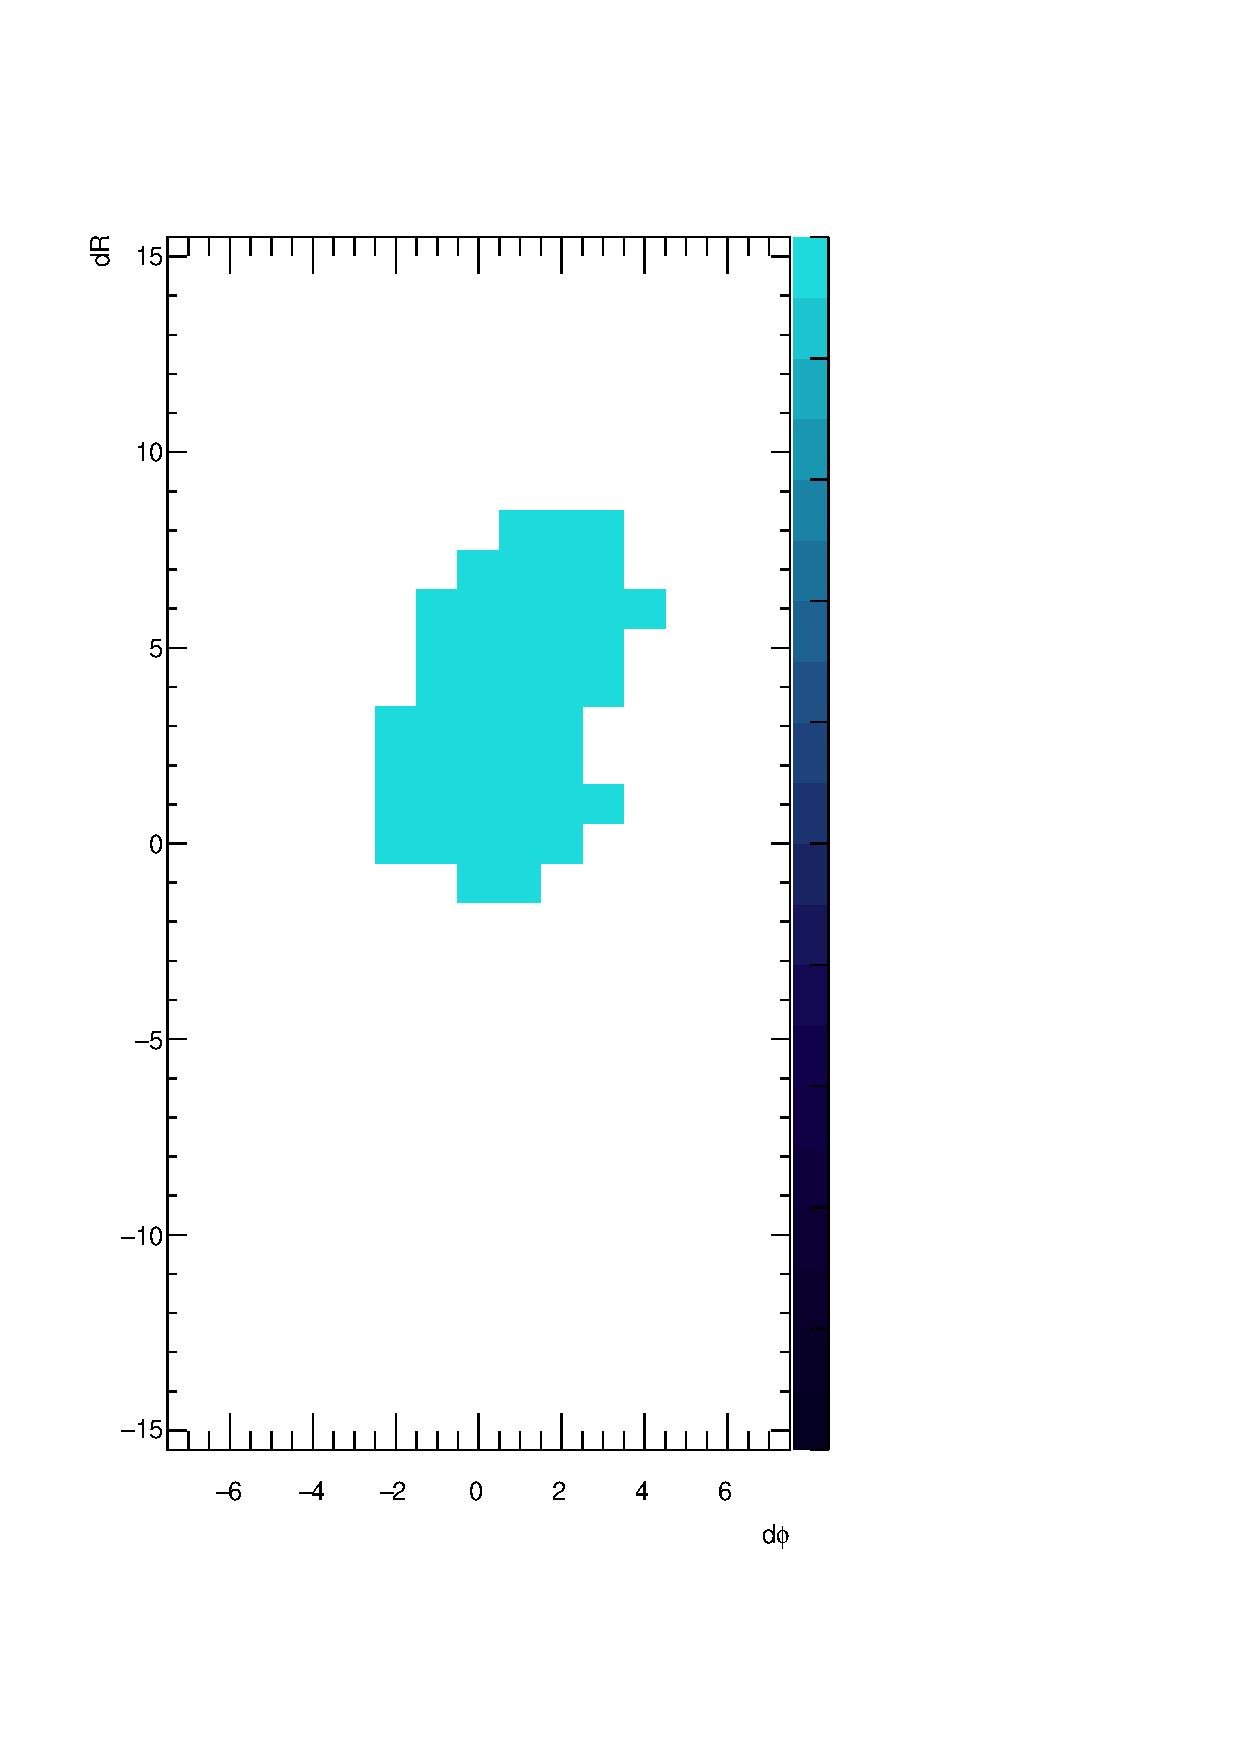
\includegraphics[clip, width=4cm]{fig/4/cut3_output.pdf}
        %\vspace{5pt}
        \subcaption{}
        \label{cut3}
    \end{minipage}%
    \end{tabular}
    \caption{MLPから出力された$p_{\rm{T}}$を任意の値で区切った時の領域。(a):出力が10.0~GeV以上の領域(b):出力が15.0~GeV(c):出力が20.0~GeV以上の領域}
    \label{ninninoCut}
\end{figure}

本研究では出力された$p_{\rm{T}}$を1~GeVから30~GeVまで0.1~GeV刻みで区切り、図~\ref{fig:ALL_Turn-on}に示すように、それぞれのTurn-on curveを導出する。そして、Turn-on curveに対してフィッティングを行い、フィッティング結果から15段階の$p_{\rm{T}}$閾値に変換を行った。
\begin{figure}[htb]
  \centering
  %\rule{8cm}{6cm}
  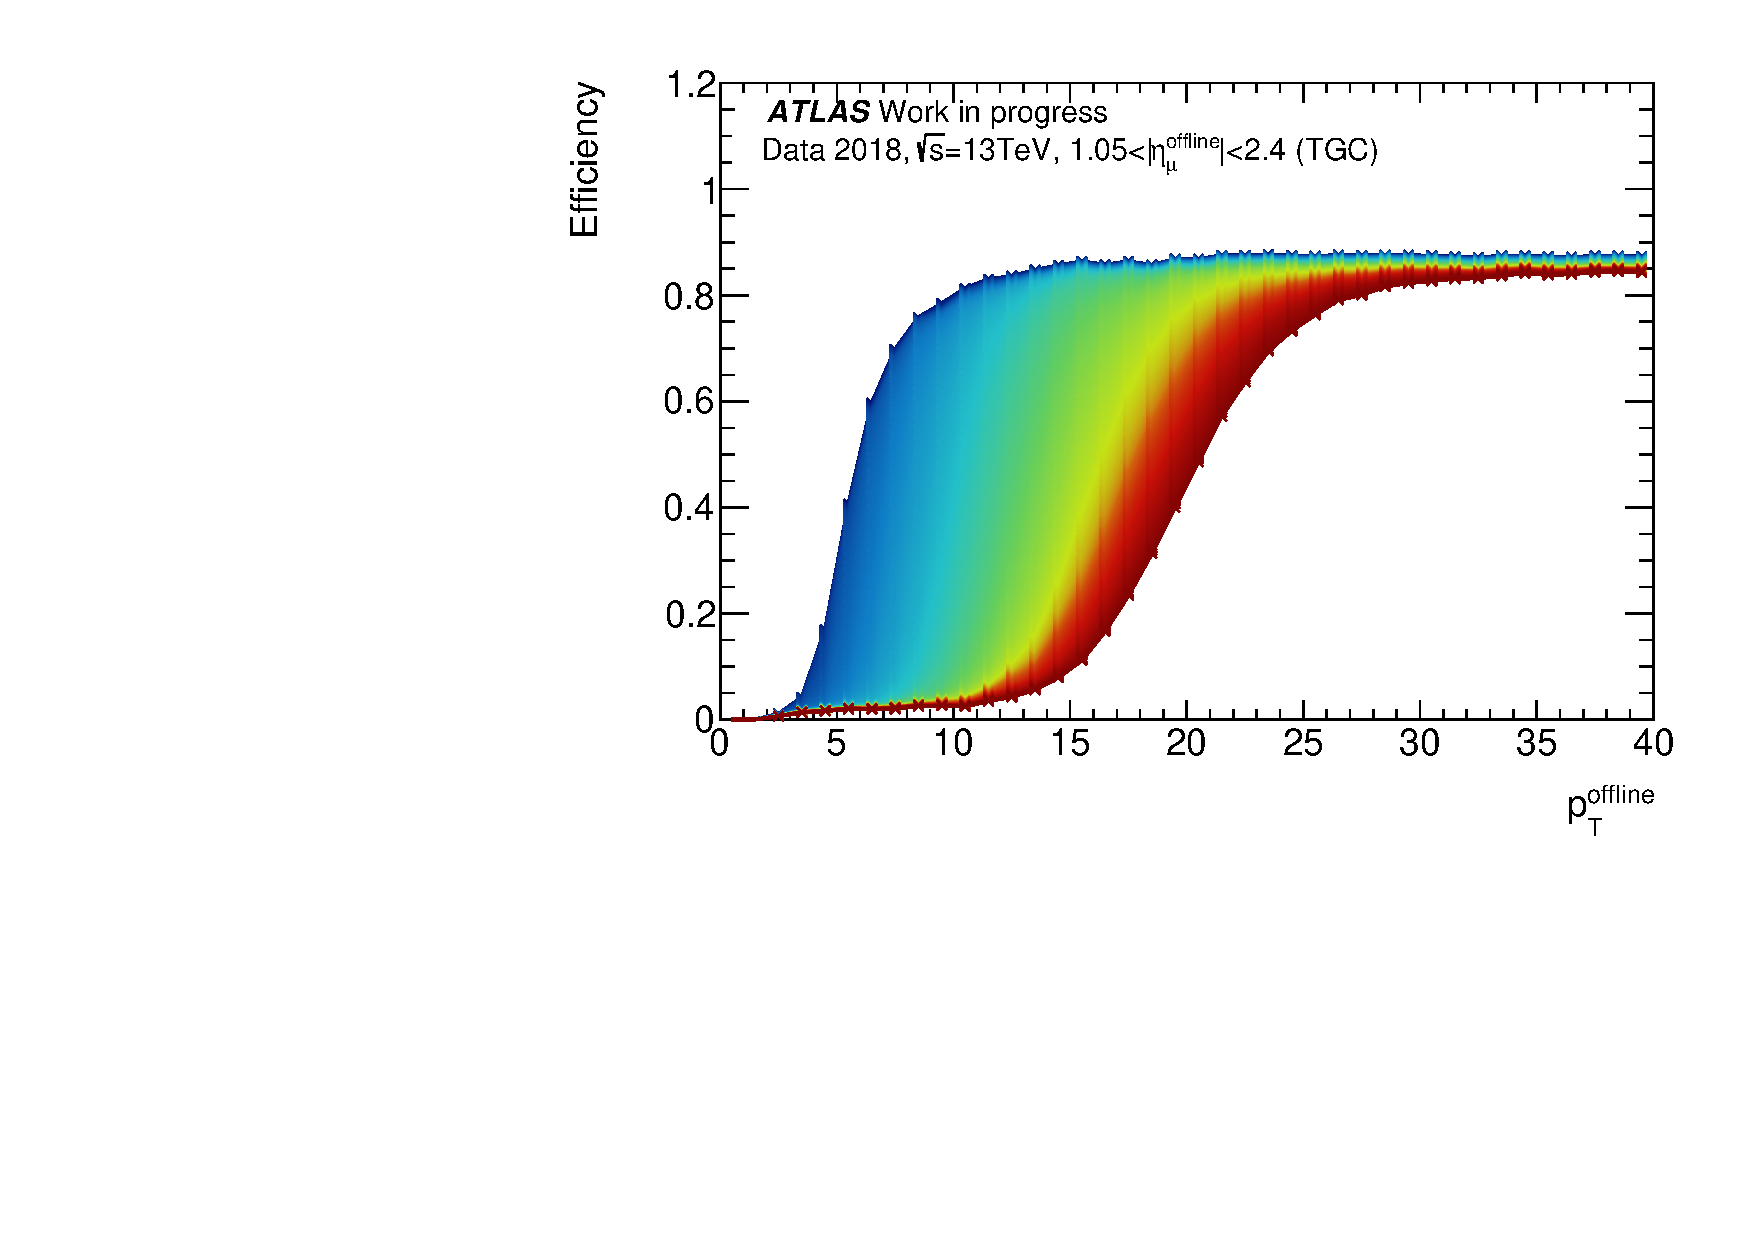
\includegraphics[clip, width=11cm]{fig/4/ALLthr_v06_Data.pdf}
  \caption{1~GeVから30~GeVまで0.1~GeV刻みで区切り、算出した300個のTurn-on curve。これらのTurn-on curveから15段階の$p_{\rm{T}}$閾値となるものを15個選ぶ。}
  \label{fig:ALL_Turn-on}
\end{figure}
図~\ref{fig:Effictive_thr_v1}にTurn-on curveにフィッティングを行って導出したEffective thresholdを示す。
$p_{\rm{T}}$が5~GeVから20~GeVまでは線形的な変換を行うことができているが、一方で$p_{\rm{T}}$が5~GeV以下の変換はできていないことが見て取れる。
これは、機械学習による低い$p_{\rm{T}}$に対するトレーニングが十分に行われていなかった可能性がある。
今後、トレーニングデータに対して$\frac{1}{p_{\rm{T}}}$の重みを付けてトレーニングを行うなどの対策によって、このような低い$p_{\rm{T}}$に対する予測性能が向上する可能性がある。
%本研究でトレーニングを行った機械学習では低い$p_{\rm{T}}$の予測が行えていない影響がしていると考えられる。

\begin{figure}[tb]
  \centering
  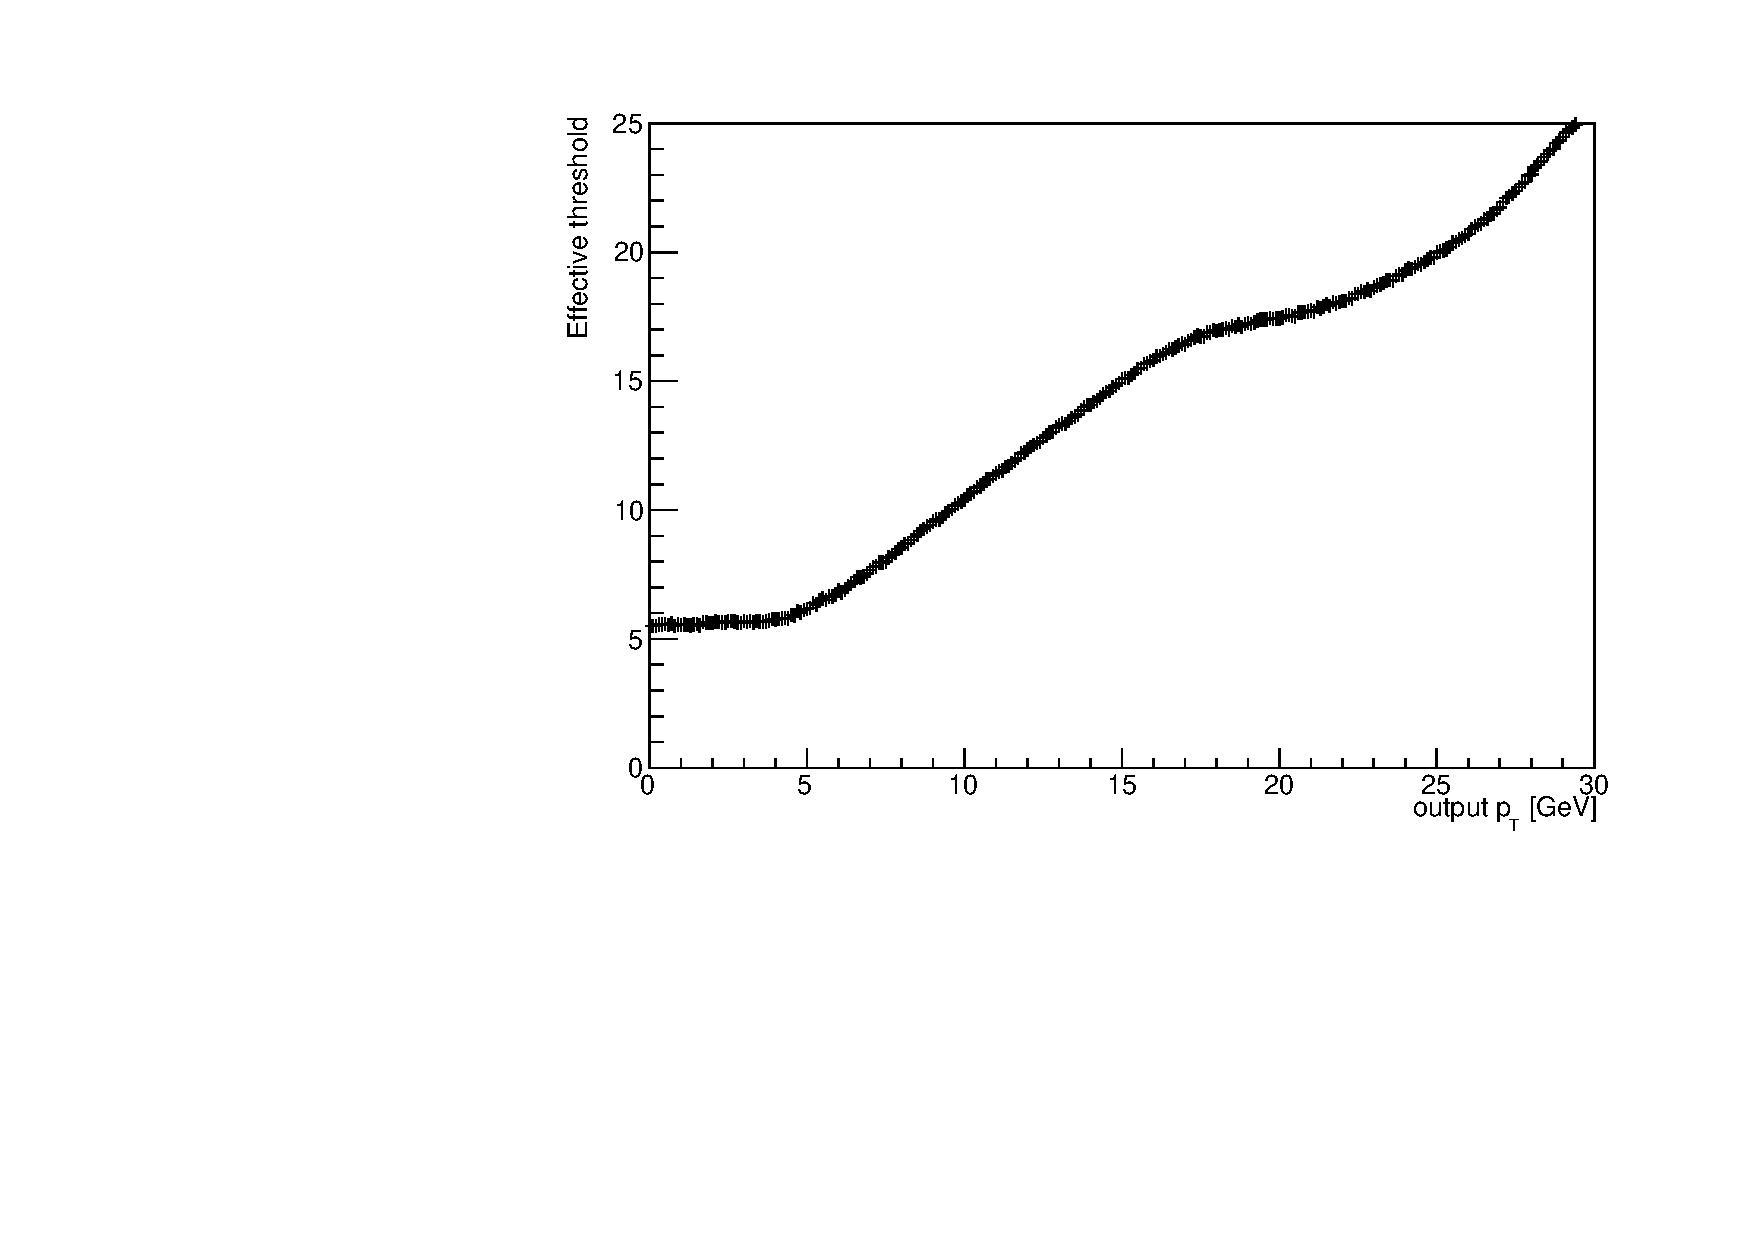
\includegraphics[clip, width=12cm]{fig/4/Effictive_thr_v1.pdf}
  \caption{出力された$p_{\rm{T}}$を0.1GeV刻みで区切った時のTurn-on curveにおけるEffective threshold。}
  \label{fig:Effictive_thr_v1}
\end{figure}

最終的に、先行研究\cite{article:shiomi-mron}で決定した$p_{\rm{T}}$閾値になるように、フィッティング結果から表~\ref{Effective_number}に示す値で15段階閾値に区切り、CWを作成した。
\begin{table}[thb]
\centering
    \caption{機械学習からの出力値におけるの15段階閾値。}
    \label{Effective_number}
    \begin{tabular}{|c|c|}
        \hline
        $p_{\rm{T}}$number & 出力された $p_{\rm{T}}$[GeV]\\
        \hline
        1 & 1.0\\
        \hline
        2 & 2.0\\
        \hline
        3 & 3.0\\
        \hline
        4 & 4.7\\
        \hline
        5 & 6.2\\
        \hline
        6 & 7.4\\
        \hline
        7 & 8.4\\
        \hline
        8 & 9.6\\
        \hline
        9 & 10.6\\
        \hline
        10 & 11.7\\
        \hline
        11 & 12.8\\
        \hline
        12 & 13.9\\
        \hline
        13 & 15.0\\
        \hline
        14 & 21.7\\
        \hline
        15 & 25.1\\
        \hline
        
    \end{tabular}
\end{table}

%図~\ref{}に本研究で作成したCWの一例を示す。




